\documentclass{article}
\usepackage[utf8]{inputenc}

\title{Causal Graphical Models }
% \author{David Johnston}

\usepackage[mathscr]{euscript}
\usepackage{natbib}
\usepackage{graphicx}
\usepackage {tikz}
\usetikzlibrary {positioning}
\usepackage[a4paper, margin=0.7in]{geometry}
\setlength{\parskip}{1em}
\setlength{\parindent}{0em}
\usepackage{amsthm}
\usepackage{amsmath}
\usepackage{amssymb}
\usepackage{dsfont}
\usepackage{hyperref}

\theoremstyle{definition}
\newtheorem{question}{Question}[section]
\newtheorem{definition}{Definition}[section]
\newtheorem{example}{Example}[section]
 
\theoremstyle{remark}
\newtheorem*{remark}{Remark}

 
\newtheorem{theorem}{Theorem}[section]
\newtheorem{corollary}{Corollary}[theorem]
\newtheorem{lemma}[theorem]{Lemma}
\newtheorem{corrolary}[theorem]{Corollary}

\setcounter{secnumdepth}{6}

\DeclareMathOperator*{\argmax}{arg\,max}
\DeclareMathOperator*{\argmin}{arg\,min}

\newcommand{\NC}[2]{\ensuremath{{#1}\not\to{#2}}}
\newcommand{\CI}{\mathrel{\text{\scalebox{1.07}{$\perp\mkern-10mu\perp$}}}}

\begin{document}

\maketitle

\tableofcontents
\newpage

%  
\section{Philosophical Preliminaries}

Causality is an imprecise concept for which various mathematical formalisations have been proposed. There is ongoing debate as to whether the mathematical formalisations adequately capture the concept. The approach here is to agnostic on the nature of causes and instead focuses on the efficacy of the mathematical formalisms in addressing particular types of query. We will call the formalisms causal models and the queries causal queries, but our relationship to the metaphysics of causality is as an inspiration for potentially useful methods rather than a true form we seek to emulate.

\section{Graphical Models}


\begin{definition}[Directed Acyclic Graph]
A Directed Acyclic Graph (DAG) $G$ is a set of vertices and directed edges $(V,E)$. A directed edge $E$ is an ordered pair of vertices $V_1$ and $V_2$, is represented by $V_1 \to V_2$ and identifies $V_1$ as a parent of $V_2$ and $V_2$ as a child of $V_1$. We say the head of $E$ points to $V_2$ and the tail points to $V_1$.
\end{definition}

\begin{definition}[Paths and Directed Paths:]
A path $p$ consists of a sequence of nodes $\mathcal{V}=\{V_i:1\leq i \leq n\}$, $n\in\mathbb{N}$ along with a sequence of edges $\mathcal{E}=\{E_i:1\leq i \leq n-1\}$. The edge $E_i$ connects nodes $V_i$ and $V_{i+1}$, no edge appears in $\mathcal{E}$ more than once and no vertex appears in $\mathcal{V}$ more than once.

A directed path is a path from $V_i$ to $V_j$ such that every edge $E_k$ is oriented from $V_k$ to $V_{k+1}$.
\end{definition}

\begin{definition}[Descendants and Ancestors]\label{def:descendants_and_ancestors}
A descendant of $V_i$ in $G$ is a child of $V_i$ or the child of a descendant of $V_i$. Equivalently, $V_j$ is a descendant of $V_i$ iff there is a directed path from $V_i$ to $V_j$.

An ancestor of $V_i$ in $G$ is a parent of $V_i$ or a parent of an ancestor of $V_i$. Equivalently, $V_j$ is an ancestor of $V_i$ iff there is a directed path from $V_j$ to $V_i$.
\end{definition}

\begin{definition}[Head-to-head node]
A head to head or collider node $V_{h}$ in a path $p$ is a node where the two adjacent edges $E_i$ and $E_{i+1}$ in $p$ are oriented as $V_{h-1}\rightarrow V_h$ and $V_h\leftarrow V_{h+1}$ respectively.
\end{definition}

\begin{definition}[Blocked path]
A path $p$ is blocked by a set $S\subset V$ iff $p$ contains a node that is not a head-to-head node that is also in $S$, or if $p$ contains a head-to-head node which is itself in $S$ or has a descendent in $S$.
\end{definition}

\begin{definition}[d-separation]
Two sets of nodes $A,B\subset V$ are d-separated in $G$ by $S\subset V$ iff every path starting with a node $A_i\in A$ and ending with a node $B_i\in B$ is blocked by $S$. We write this relation $A \perp_G B | S$.
\end{definition}

\section{Probability distributions, marginals and conditionals}

All definitions are for discrete probability spaces. I will extend them to continuous spaces when it becomes necessary.

\begin{definition}[Probability Space]
A probability space is a triple $(\Omega,\mathcal{F},P)$, where $\Omega$ is an arbitrary sample space, $\mathcal{F}$ is a $\sigma$-algebra on $\Omega$ and $P:\mathcal{F}\to[0,1]$ satisfies the properties of a measure over $\mathcal{F}$ as well as $P(\Omega)=1$.
\end{definition}

\begin{definition}[Random varible]
Given a probability space $(\Omega,\mathcal{F},P)$ and a measurable space $(E,\mathcal{E})$, a random variable is a measurable function $X:\Omega\to E$.

Abusing notation somewhat, we will write $P(X\in B)$ to mean $P(X^{-1}(B))$ for $B\in\mathcal{E}$. 

We will write the $\sigma$-algebra associated with a random variable $X$ as $\sigma(X)$. We will also sometimes discuss the range of values $X$ may take, denoted by $\text{Range}(X)$.
\end{definition}

\begin{definition}[Probability distribution]
Given a random variable $X$ associated with a probability space $(\Omega,\mathcal{F},P)$, the probability distribution of $X$ is the map $f:\sigma(X)\to [0,1]$ such that $f(B)=P(X\in B)$ for $B\in\sigma(X)$. We will write the probability distribution over $X$ as $P(X)$.

For random variables $X$, $Y$ associated with measure spaces $(D,\mathcal{D})$ and $(E,\mathcal{E})$, $P((X\in B)\wedge (Y \in C))$ for $B\in\mathcal{D}$, $C\in\mathcal{E}$ means $P(X^{-1}(B)\cap Y^{-1}(C))$, and we write the distribution over $X$ and $Y$ as $P(X\wedge Y)$.

\end{definition}

For the following definitions, assume we have a set of random variables $V$ and a probability space with measure $P$:

\begin{definition}[Conditional probability]
For a finite probability space, the conditional probability $P(V\setminus S|S\in s):\sigma(V\setminus S)\to [0,1]$ is \[P(V\setminus S|S\in s)=\frac{P(V)}{P(S\in s)}\]

For finite probability spaces, the conditional probability is undefined if $P(S\in s)=0$.

TBD: conditioning on probability 0 events in infinite spaces.
\end{definition}

\begin{definition}[Marginal probability]
The marginal probability of $A\subset V$, $P(A):\sigma(A)\to [0,1]$ is \[P(A):=\sum_{v\in \sigma(V\setminus A)} P(A \wedge V\setminus A \in v)\]
\end{definition}

\begin{definition}[Independence]
$A\subset V$ and $B\subset V$ are independent iff $P(A\wedge B)=P(A)P(B)$. We write independence $A\CI_{P(V)} B$.
\end{definition}

\begin{definition}[Conditional independence]
Given $A, B, S \subset V$, $A$ is conditionally independent of $B$ given $S$ iff $A\CI_{P(V\setminus S|S\in s)} B$ for all $s\in\sigma(S)$. We write this $A\CI_P B | S$.
\end{definition}

\section{Faithfulness}
\begin{remark}
Compatibility and faithfulness are both standard definitions, transparency is not. I chose transparency for the connotation that "the probability distribution doesn't mislead you with spurious independences".
\end{remark}

\begin{definition}[Compatibility]\label{def:compatibility}
A probability distribution $P$ is compatible with a DAG $G$ iff $A\perp_G B |S \Rightarrow A\CI_P B | S$ for all $A, B, S \subset V$.

Another term for compatibility is \emph{Markovian}
\end{definition}

\begin{definition}[Transparency]
A probability distribution $P$ is transparent with respect to a DAG $G$ iff $A\CI_P B|S \Rightarrow A\perp_G B|S$ for all $A,B,S\subset V$.
\end{definition}

\begin{definition}[Faithfulness]\label{def:faithfulness}
A probability distribution $P$ over variables $V$ is faithful to a DAG $G$ over vertices $V$ iff $A \CI_P B | S \Leftrightarrow A\perp_G B | S$ for all $A,B,S\subset V$.
\end{definition}

From these definitions, $\text{Transparency}+\text{Compatibility}\Leftrightarrow \text{Faithfulness}$. Any distribution $P$ is compatible with a fully connected graph and transparent with respect to a fully disconnected graph, but some distributions have no graph to which they are faithful.

A graph $G$ may not permit faithfulness of some probability distribution $P$ simply by including spurious arrows. For example, if $A\CI_P B | \varnothing$, the graph $G=(\{A,B\},A\to B)$ is compatible but not faithful to $P$, and we can create a faithful graph by removing the edge $A\to B$.

It is also possible, however, that a graph can fail to be faithful in a manner that cannot be resolved by removing an edge (see Example \ref{ex:linear_unfaithfulness}). The strictly weaker condition of \emph{minimality} captures the intuition of "a graph without superfluous arrows".

\begin{definition}[Minimality]\label{def:minimality}
A graphical model of a Markovian probability distribution over random variables $\mathbf{V}$ is minimal if, for every $V_i\in\mathbf{V}$ and every parent $p$ of $V_i$
\[V_i\not\CI p|\mathrm{Parents}(V_i)\setminus p\]
\end{definition}


\subsection{Directed Markov properties}

A probability distribution $P$ that is compatible with a DAG $G$ satisfies a number of equivalent properties in addition to the $d$-separation condition given in Defintion \ref{def:compatibility} (proofs omitted).

\begin{definition}[Markov factorisation]\label{def:markov_factorisation}
If $P$ is compatible with $G$, then we can write
\begin{align}
    P(V) = \prod_{V_i\in V} P(V_i|\mathrm{pa}_i)
\end{align}
Where $\mathrm{pa}_i$ is the set of parents of $V_i$ in $G$
\end{definition}

\begin{definition}[Local directed Markov property]\label{def:local_markov}
Denote by $\mathrm{nd}_i$ the set of all non-descendents $\mathrm{nd}_i=V\setminus (\mathrm{de}_i\cup\{V_i\})$.

Then, given $P$ compatible with $G$,
\begin{align}
    V_i \CI_P \mathrm{nd}_i | \mathrm{pa}_i
\end{align}
\end{definition}




\section{Additional Definitions}

\begin{definition}[Markov equivalence class]
The Markov equivalence class $\mathcal{M}_G$ of graph $G$ is the set of graphs which share d-separation properties with $G$: $\mathcal{M}_G=\{G'\in\mathcal{G}:A\perp_{G'}B | S \Leftrightarrow A\perp_{G}B|S\}$. In other words, given the set of distributions $\mathcal{P}_G:=\{P|P\text{ is faithful to }G\}$, the Markov equivalence class of $G$ is the set of all graphs to which every distribution in $\mathcal{P}_G$ is faithful.
\end{definition}

\begin{definition}[Markov superclass]
The Markov superclass $\mathcal{M}_G$ of graph $G$ is the set of graphs $\{G'|A\perp_{G'} B \implies A\perp_G\}$. In other words, the Markov superclass of $G$ is the set of all graphs compatible with probability distributions that are compatible with $G$. 
\end{definition}

\begin{definition}[Structural equation model]\label{def:structural_equation}
Given a set of random variables $\mathcal{X}=\{X_i$\}, define $\mathcal{X}_{<n}=\{X_i|i<n\}$. A structural equation model is a set of assignments for each $i\in\{1,...,n\}$ of the form

\begin{align*}
    X_n &:= f_n(Q_{<n},u_{X_n})
\end{align*}

Where $Q_{<n}\subset \mathcal{X}_{<n}$ and $u_{X_i}$ are random variables usually assumed to be jointly independent with associated distributions $\mathcal{L}(u_{X_i})$. 
\end{definition}

\begin{definition}[Corresponding graph]\label{def:sem_corresponding_dag}
The corresponding graph for a SEM is the DAG $G=(V,E)$ where $X_i\to X_j\in E$ iff $X_i$ appears on the right hand side of the assignment for $X_j$.
\end{definition}

\section{Faithfulness properties of Structural Equation Models}

\subsection{SEM + joint independence of noises $\Rightarrow$ compatibility}

Joint independence of the noises $E_{X_i}$ is sufficient to ensure that the probability distribution defined by such a SEM is compatible with a DAG constructed via Definition \ref{def:sem_corresponding_dag} \cite{spirtes_causation_1993} (pp41). The argument involves showing that conditioning on variables on the right hand side of an assignment in an SEM create independences, and that these independences map to d-separation in the related DAG.

\subsection{SEM + joint independence of noises $\not\Rightarrow$ transparency}

Here we show by way of example that a probability distribution defined by a SEM with jointly independent noises can fail to be faithful to a DAG constructed as above.

\begin{example}\label{ex:linear_unfaithfulness}
Consider the following assignments constituting a structural equation model over $\{X_1,X_2,X_3\}$
\begin{align*}
    X_1 &:= u_{X_1} \\
    X_2 &:= a X_1 + u_{X_2} \\
    X_3 &:= b X_1 + c X_2 + u_{X_3}
\end{align*}

Following Definition \ref{def:sem_corresponding_dag}, the corresponding DAG to this assignment is:

\begin {center}
\begin {tikzpicture}[-latex ,auto ,node distance =4 cm and 5cm ,on grid ,
semithick ,
state/.style ={ circle ,top color =white ,
draw , text=blue , minimum width =1 cm}]
\node[state] (A) [left] {$X_1$};
\node[state] (B) [right = of A] {$X_2$};
\node[state] (C) [below = of B] {$X_3$};
\path (A) edge [] node[above] {} (C);
\path (A) edge [] node[above] {} (B);
\path (B) edge [] node[above] {} (C);
\end{tikzpicture}
\end{center}

A probability distribution transparent with respect to this DAG would have no conditional independences, as this DAG features no d-separation. However, if $ac=-b$, the assignments above reduce to 

\begin{align*}
    X_1 &:= E_{X_1} \\
    X_2 &:= a X_1 + E_{X_2} \\
    X_3 &:= c E_{X_2} + E_{X_3}
\end{align*}

By the assumption of jointly independent noises, under this assignment we will have $X_3 \CI_P X_1 | \varnothing$, and so this model fails to be transparent with respect to the DAG illustrated above.
\end{example}

\section{Faithfulness as nongenericity}

Assuming faithfulness can be justified by the argument that, under certain conditions, faithfulness is only violated by probability distributions that are nongeneric.

Take the set of all DAGs $\mathcal{G}$ over vertices indexed by $i\in\{1,..,n\}$ and an arbitrary set of probability distributions $\mathcal{P}$ over random variables $V=\{V_i|i\in\{1,..,n\}\}$. Assume for each graph $G$ there is an associated measure $\mu_G$ over a $\sigma$-algebra on $\mathcal{P}$.

A contrast is a function $C:\mathcal{P}\to\mathbb{R}^n$.

A distribution $P$ is generic relative to $\mu_G$, $C$ if

\begin{align*}
    \mu_G(\{P':C(P')=C(P)\}) \neq 0
\end{align*}

Consider the contrast:
\[C_{FF}(P) = [\mathds{1}_{X\CI_P Y|S}|X,Y\in V,S\subset V]\]

Where $\mathds{1}_s$ is a function that evaluates to $1$ if $s$ is true and $0$ otherwise, and $\rho_{XY|S}$ is the partial correlation of $X$ and $Y$ controlling for $S$.

For each graph $G$ we can construct a vector 
\[\text{Sep}(G) = [\mathds{1}_{X\perp_G Y|S}|X,Y\in V, S\subset V]\]

The vectors $C_{FF}(P)$ and $\text{Sep}(G)$ represent the conditional independence properties of $P$ and the d-separation properties of $G$ respectively. They are defined such that $C_{FF}(P)=\text{Sep}(G)\Leftrightarrow P\text{ is faithful to }G$ (this is a straightforward consequence of Definition \ref{def:faithfulness}.

Under some additional assumptions, the $\{P|C_{FF}(P)=\text{Sep}(G)\}$ also characterises the set of distributions $\mathbf{P}_G\subset \mathcal{P}$ which are generic with respect to $C_{FF}$ and the measure $\mu_G$. Examples of these assumptions are given below, with proofs given in the referenced literature.

Take $\mathcal{P}$ to be the space of multivariate Gaussians with parametrisation $\mathbf{\theta}\subset \mathbb{R}^{|V|^2}$ and each $\mu_G$ a probability measure such that, for any set of parametrisations $\Theta\subset \mathbb{R}^{|V|^2}$ with Lebesgue measure zero, the measure of the associated set of distributions $\mu_G(\mathbf{P}^\Theta)=0$. It has been shown that, given these assumptions, all distributions in $\mathbf{P}_G$ are generic with respect to $C_{FF}$ and $\mu_G$, while any distributions not in $\mathbf{P}$ are nongeneric \cite{spirtes_causation_1993} (pp41-2). It has also been shown that an analogous result holds for discrete distributions \cite{meek_strong_2013}.

In the infinite sample case, these arguments motivate the use of the faithfulness assumption:
\begin{enumerate}
    \item If we accept that the class of measures $\mu_G$ that respect the assumption regarding a density on $\theta$ contains the probability distribution of cause-effect relationships in nature, then assuming faithfulness will reject a correct graph with probability 0
    \item The faithfulness assumption allows us to reject all graphs outside of a single Markov equivalence class, which will usually reduce the set of causal models that we hypothesise may generate the data
\end{enumerate}

Regarding the "usually" on the second point above, if the Markov equivalence class accepted is fully connected, then there is no restriction on the probability distribution implied. On the other hand, if faithfulness is assumed there may be a restriction on possible interventional distributions (i.e. distributions under $do()$ interventions) - I don't know at this point.

All these points have been discussed in the literature, bar the formulation in terms of a contrast and the final comment about whether fully connected graphs imply restrictions on interventional distributions if faithfulness is assumed.

\begin{remark}
A corollary of this is that a probability distribution $P$ that is faithful to a graph $G$ is not only generic with respect to $C_{FF}$ and $\mu_G$, but also nongeneric with respect to $C_{FF}$ and $\mu_{G'}$ for any $G'$ not in the Markov equivalence class of $G$.
\end{remark}

% Questions I'm interested in pursuing:
% \begin{itemize}
%     \item What is the appropriate way to formulate the two items in the list above in a more rigorously? Is it possible to produce "performance metrics" for causal discovery rules based on these items?
%     \item Assuming a measure of performance and dropping the infinite sample assumption, can we retain a general class of priors $\mu_G$ that will guarantee reasonable performance of causal discovery based on the faithfulness assumption? 
%     \item Can the two questions above be applied to other causal discovery rules?
% \end{itemize}


\section{Causal models}

In this section I propose a general definition of causal models and fit various existing definitions into this one.

\begin{definition}[Causal model]
Given a set $\mathbf{V}$ of random variables and a set $\mathcal{I}$ of interventions, a causal model is a map $M:\mathcal{I}\to \mathcal{P}(\mathbf{V})$ where $\mathcal{P}(\mathbf{V})$ represents the set of all probability distributions over $\mathbf{V}$.

To reflect notation used in other literature, I will sometimes use $P_I$ to represent the probability distribution $M(I)$.
\end{definition}

\begin{remark}
A causal model so defined is similar to a conditional distribution. There is an intuitive sense in which $P(V|I)$ means the same thing as $M(I)$. However, unlike the conditional $P(V|I)$, a causal model doesn't require the joint distribution $P(V,I)$ to be well defined.
\end{remark}

\subsection{Cause and effect models}

A particular class of causal model is built on the notion of cause-effect relationships. A cause-effect relationship is a directed binary relation. For a set of variables $V$, we also require that the set of causal relations between them doesn't induce any cycles. It may be the case that for some systems of interest there are no acyclic cause-effect assignments that yield a reasonable causal model; for such systems, we will have to consider a broader class of causal models. 

Given the assumptions above, the cause-effect relationships of a cause-effect model form a directed acyclic graph (DAG) over the model's variables. One fact to bear in mind in the following discussion is that there are two types of DAGs that are often discussed in relation to causal inference. The first, sometimes termed a Bayesian network, is a DAG $G=(V,E)$ which is compatibile with the probability distribution $P$ over variables we identify with the nodes $V$ (see Definition \ref{def:compatibility}). Sometimes, a Bayesian network might additionally be supposed to be minimal or faithful to $P$ (see Definitions \ref{def:minimality} and \ref{def:faithfulness}). In all cases, there are usually several graphs $G$ which bear the appropriate relations to $P$.

The second, which we will call a causal graph, is related to a full causal model $M$ rather than a single probability distribution $P$. Under some assumptions, the causal graph for a model $M$ is unique (see \ref{th:unique-minimal-graph}). 

\begin{definition}[Direct causes and effects]
A cause-effect relationship is a directed binary relation $\rightsquigarrow$. Given $V_i\rightsquigarrow V_j$, we say $V_i$ is a direct cause of $V_j$ and $V_j$ is a direct effect of $V_i$.

For a set of variables $\mathbf{V}$, cause-effect relationships $E$ and $V_i\in\mathbf{V}$, write  the set of direct causes of $V_i$ as $\mathrm{dc}_i=\{V_j|(V_j\rightsquigarrow V_i)\in E\}$ and the set of direct effects as $\mathrm{de}_i=\{V_j|(V_i\rightsquigarrow V_j)\in E\}$.
\end{definition}

\begin{definition}[Causes and effects]
A set of cause-effect relationships $E$ over variables $V$ induces a directed graph $G=(V,E)$. 

A cause of a variable $V_i$ is an ancestor of $V_i$ in $G$, and an effect of $V_i$ is a descendant of $V_i$. See Definition \ref{def:descendants_and_ancestors}.

Write the set of causes of $V_i$ as $\mathbf{c}_i$ and the set of effects as $\mathbf{e}_i$.

\end{definition}

\begin{definition}[Noneffects]
Define the noneffects of $V_i\in\mathbf{V}$ as $\mathrm{ne}_i:= (\mathbf{e}_i\cup \{V_i\})^C$.
\end{definition}

\begin{definition}[Causal Markov Condition (CMC)]
A probability distribution $P$ is Markov with respect to a cause-effect graph $G=(\mathbf{V},E)$ if it satisfies any of the equivalent conditions of compatibility (Def \ref{def:compatibility}), Markov factorisation (Def \ref{def:markov_factorisation}) or the local Markov property (Def \ref{def:local_markov}).

The CMC is typically stated in terms of the local Markov property:
\begin{align}
    V_i\CI_P \mathrm{ne}_i | \mathrm{dc}_i
\end{align}
\end{definition}

Along with the assumption of acyclicity, CMC is equivalent to the property that the probability distribution $P$ is consistent with $G$ (i.e. d-separation in $G$ implies conditional independence in $P$). 


\begin{definition}[Markovian cause effect model]
A causal model $M$ along with a directed acyclic graph $G$ for which every $P\in \mathrm{Range}(M)$ is Markovian with respect to $G$ is a Markovian causal model.
\end{definition}

\subsection{Causal Bayesian networks}

Here I will define causal Bayesian networks (CBNs), a particular case of Markovian cause effect models. These are Bayesian networks with the "do" operator of the type discussed by Pearl.

A CBN $M$ is defined via the operation of $M$ on allowable interventions $I$. We will first define the notation and spaces for these interventions, and then the restrictions on the operation of $M$ required by a CBN.

\begin{definition}[Atomic intervention (CBN)]
Given a CBN $M$ over a set of random variables $V$, an atomic intervention is an index $i$ along with an element of the range of the corresponding variable $V_i$. Given $i\in\{0,..,|V|\}$, the atomic intervention $I_i \in \{i\}\times \text{Range}(V_i):=\mathcal{I}_{i}$. 

We can write atomic interventions in two ways $I:=[i,v_i]\equiv do(V_i=v_i)$.

% Given an atomic interventions $I_i \in \mathcal{I}_{i}$, a CBN $M$ has the following property for some probability distribution $Q$:
% \begin{align}
%         I_{i} = [i,v_i] \implies M(I_{i}) = \delta(V_i-v_i)Q(V\setminus \{V_i\})
% \end{align}
\end{definition}

\begin{definition}[Intervention (CBN)]
An intervention $I_U$ on a set of variables $V$ is defined as the union over any set of atomic interventions on the variables of $V$: 
\[I_U=\cup_{i\in U\subset \{1,..,V\}} I_{i}\]

Define the intervention space $\mathcal{I}_U:=\prod_{i\in U} \mathcal{I}_i$
\end{definition}

\begin{definition}[Passive intervention (CBN)]
Define the passive intervention $I_0:=\varnothing$.
\end{definition}

\begin{definition}[Intervention space (CBN)]\label{def:cbn_intervention_space}
The space of permissible interventions for a CBN is $\mathcal{I} := I_0\cup \left(\cup_{U\in\mathds{P}(\{1,..,|V|\})}\right)$
\end{definition}

\begin{definition}[Target variables]
For an intervention $I_U = \cup_{i\in U} I_{i}$, we call the set $V_U = \{V_i|i\in U\}$ the target variables.
\end{definition}

\begin{definition}[Causal Bayesian Network]
Consider the set of interventions $\mathcal{I}$ and a causal model $M:\mathcal{I}\to\mathcal{P}$ over random variables $V$, and write $P_A=M(I_A)$. $M$ is a Causal Bayesian Network if
\begin{enumerate}
    \item There is some cause-effect graph $G=(V,E)$ such that $M$ is Markovian relative to $G$ and
    \item For intervention $I_U$ and any $V_i \in \{V_k|k\in U\}^C$, $P_U(\mathrm{dc}_i) > 0 \implies P_U(V_i|\mathrm{dc}_i) = P_0(V_i|\mathrm{dc}_i)$ where $\mathrm{dc}_i$ is defined relative to $G$
    \item $I_U = \cup_{i\in U}[i,v_i] \implies P_U(\{V_i|i\in U\}) = \prod_{i\in U} \delta_{V_iv_i}$
\end{enumerate}
Here $\delta_{ij}$ is the Kronecker delta function, defined such that $\delta_ij=0$ for $i\neq j$ and $\delta_{ii} = 1$.

Call any graph $G$ for which properties 1 \& 2 hold the \emph{associated graph}.
\end{definition}

\begin{definition}[Truncated factorisation]
A causal model $M$ obeys truncated factorisation relative to a graph $G$ if, for every $I_U=\cup_{i\in U} [i,v_i]$, the distribution $P_U$ can be written as product of the conditionals of non-target variables under the ``null intervention'' distribution $P_0$ and delta functions over the target variables:
\[P_U(\mathbf{V}) = \prod_{i\in U} \delta (V_i-v_i)\prod_{i\not\in U} P_0(V_i|\mathrm{dc}_i) \]
\end{definition}

\begin{theorem}[CBN satisfies truncated factorisation]
A CBN has the truncated factorisation property.
\end{theorem}

\begin{proof}
$M(I_U)$ is Markov with respect to an associated graph $G$ for any $I_U$, and so it is possible to write
\begin{align}
    P_U(\mathbf{V})  &=  \prod_{i\in\{1,..,|V|\}} P_U(V_i|\mathrm{dc}_i) \nonumber \\
    &=  \prod_{i\in U} P_U(V_i|\mathrm{dc}_i) \prod_{i\not \in U} P_U(V_i|\mathrm{dc}_i) \label{eq:markov_factorisation_split}
\end{align}
with $\mathrm{dc}$ defined relative to $G$.

By property 3 of a CBN, $I_U =\cup_{i\in U}[i,v_i] \implies P_U(V_i=v_i)=1$ and $P_U(V_i\neq v_i)=0$ for all $i\in U$. Noting that $P(A)=0$ implies $P(A|X)=0$ and $P(A)=1$ implies $P(A|X)=1$ for any $X$ of nonzero probability, so $P(A)=\delta_{Aa}\implies P(A,B)=\delta_{Aa}P(B)$. Direct substitution into Eq. \ref{eq:markov_factorisation_split} yields

\[P_I(\mathbf{V}) = \prod_{i\in U} \delta(V_i-v_i)\prod_{i\not\in U} P_U(V_i|\mathrm{dc}_i) \]

Applying property 2, we have

\[P_I(\mathbf{V}) = \prod_{i\in U} \delta(V_i-v_i)\prod_{i\not\in U} P(V_i|\mathrm{dc}_i) \]

\end{proof}

\begin{definition}[Graphical truncation]
Given an intervention space $\mathcal{I}$ and the set of all directed acyclic graphs $\mathcal{G}$ over nodes indexed by $i\in\{1,..,n\}$, graphical truncation is the operation $T:\mathcal{I}\times\mathcal{G}\to\mathcal{G}$ that takes a graph $G=(V,E)$ and intervention $I_U$, and returns the graph $G_U=(V,E_U)$ where $E_U=\{(V_i\to V_j)|(V_i\to V_j)\in E\text{ and }j\not\in U\}$.
\end{definition}

\begin{corollary}[CBN satisfies graphical truncation]
A CBN $M$ with an associated graph $G$ has the property that for every $I_U\in\mathcal{I}$, $P_U$ is Markovian relative to the truncated DAG $G_U:=T(I_U,G)$.
\end{corollary}

The required conditional independences are a direct result of the truncated factorisation property.

\begin{remark}
Conditions 1 and 2 are not on their own sufficient for graphical truncation.

Example: Consider a two variable Markovian causal model $M$ with $G=(\{X,Y\},\{X\rightsquigarrow Y\})$. Chose some distribution $P_0(X,Y)$ for which $X\not\CI_{P_0} Y| \varnothing$. Clearly, $P(X,Y)$ is Markov with respect to $G$. Consider an intervention $I$ which targets $Y$ such that $M(I)=P_I(X,Y)=P_0(X,Y)$. $P_I(X,Y)$ is trivially also Markov with respect to $G$, and $P_I(X)=P(X)$, however $X\not\CI_{P_I} Y| \varnothing$.
\end{remark}

\begin{remark}
It is straightforward to show that truncated factorisation implies conditions 2 and 3, so an alternative definition of CBNs would be to replace conditions 2 and 3 with truncated factorisation instead.

It is also possible to define weaker truncated factorisation schemes, for example we could require 
\begin{align}
    P_U(\mathbf{V})  &=  \prod_{i\in U} P_U(V_i) \prod_{i\not \in U} P(V_i|\mathrm{dc}_i)
\end{align}
that will respect graphical truncation, or
\begin{align}
    P_U(\mathbf{V})  &=  \prod_{i\in U} P_U(V_i|\mathrm{dc}_i) \prod_{i\not \in U} P(V_i|\mathrm{dc}_i)
\end{align}
that will not.
\end{remark}

As mentioned earlier, while a Bayesian network usually does not have a unique graph, even if we require minimality or faithfulness. A causal Bayesian network, on the other hand, has a unique minimal associated graph.

\begin{lemma}[$G$ is minimal $\implies T(I,G)$ is minimal]\label{lem:universal_minimality}
Given a CBN $M$ and an associated graph $G$ that is minimal with respect to $P_0$, $G_U$ is minimal with respect to $P_U$ for all interventions $I_U$.
\end{lemma}

\begin{proof}
We will proceed by showing $G_U$ is not minimal with respect to $P_U \implies G$ is not minimal with respect to $P_0$.

Suppose $G_U$ is not minimal with respect to $P_U$ for some $I_U\in\mathcal{I}$. Then there is some node $V_i\in \mathbf{V}$ with parent $p$ such that $V_i \CI_{P_U} p | \mathrm{dc}_i\setminus \{p\}$. Thus $P_U(V_i|\mathrm{dc}_i) = P_U(V_i|\mathrm{dc}_i\setminus \{p\})$. If $i\in U$, the parent set of $V_i$ would be empty in $G_U$, so we can exclude this possibility. If $i\not \in U$, we have $P_U(V_i|\mathrm{dc}_i)=P_0(V_i|\mathrm{dc}_i)$, and so $V_i\CI_{P_0} p|\mathrm{dc}_i\setminus \{p\}$. Thus $G$ is not minimal with respect to $P_0$.
\end{proof}

\begin{lemma}[Reduction to minimal graph]\label{lem:reduction_minimal}
Given a CBN $M$ and an associateg graph $G$, a minimal graph $G^*$ can be generated by removing edges from $G$.
\end{lemma}

\begin{proof}
If a graph is not minimal with respect to $P_0$, it is possible to identify a node $V_i$ with a parent $p$ such that \[V_i\CI_{P_0} p|\mathrm{dc}_i\setminus \{p\}\]

Consider the graph $G'$ created by removing the edge $p\to V_i$ from $G$. We will show that $M(I)$ satisfies the local Markov property with respect to $G'$ for all interventions $I$.

First, by the local Markov property on $P_U=M(I_U)$ and $G$, we have $V_i \CI_{P_U} \mathrm{ne}_i|\mathrm{dc}_i$. In addition, by assumption, $V_i\CI_{P_0} p|\mathrm{dc}_i\setminus \{p\}$. The contraction property of conditional independence then gives us $V_i \CI_{P_U} \mathrm{ne}_i\cup\{p\}|\mathrm{dc}_i\setminus\{p\}$. Noting that $\mathrm{ne}_i\cup\{p\}$ is the set of noneffects of $V_i$ in $G'$ and $\mathrm{dc}_i\setminus \{p\}$ is the set of direct causes in $G'$, we have verified the local Markov property as required.
\end{proof}

\begin{theorem}[A CBN has a unique minimal associated graph]\label{th:unique-minimal-graph}
Given a CBN $M$ with an associated graph $G$, there is a unique graph $G^*$ that is minimal with respect to $P_0$ and for which $T(I_U,G^*)$ is minimal with respect to $P_U$.
\end{theorem}

\textbf{Proof:} Construct a minimal graph $G^*$ from $G$ by removing any edges necessary. By Lemmas \ref{lem:universal_minimality} and \ref{lem:reduction_minimal}, $G^*$ produces minimal graphs compatible with $P_U$ under graphical truncation with $I_U$.

Suppose there is a graph $G'$ that disagrees with $G^*$ on at least one edge that also generates a set of graphs that render $M$ Markovian.

Suppose that an edge disagreement is between nodes $V_i$ and $V_j$. We will identify three cases:
\begin{enumerate}
    \item There is an edge between $V_i\to V_j$ in $G^*$, and no edge in $G'$
    \item There is no edge between $V_i$ and $V_j$ in $G^*$, and there is an edge $V_i\to V_j$ in $G'$
    \item There is an edge $V_i \to V_j$ in $G^*$, and an edge $V_j\to V_i$ in $G'$
\end{enumerate}

In case (1), consider $I_{\mathrm{ce}_j^{G^*}}$, an intervention on the direct causes and effects of $V_j$ with respect to $G^*$.  If $G'_{\mathrm{ce}_j^{G^*}}$ were Markov with respect to $P_{\mathrm{ce}_j^{G^*}}$, then we would have $V_i \CI_{P_{{\mathrm{ce}_j^{G^*}}}} V_j | \mathrm{dc}^{G^*}_{V_j}\setminus \{V_i\}$. This would imply that $G^*_{\mathrm{ce}_j^{G^*}}$ is not minimal with respect to $P_{\mathrm{ce}_j^{G^*}}$, contradicting Lemma \ref{lem:universal_minimality}.

In case (2), either $V_i$ is a descendent of $V_j$ in $G^*$, $V_j$ is a descendent of $V_i$ or neither are descended from the other. 

First, suppose $V_j$ is a descendent of $V_i$ in $G^*$. Then, by the local Markov property, $V_i\CI_{P_0} V_j | \mathbf{V}^{pa}_j$, as $V_j$ must be a nondescendent of $V_i$ by acyclicity. Then $V_i\to V_j$ in $G'$ violates minimality of $G'$. 

Next, suppose $V_i$ is a descendent of $V_j$ in $G^*$. Because $G'$ is acyclic, $V_i$ cannot be a descendent of $V_j$ in $G'$. Thus we can identify two nodes $V_k$ and $V_l$ such that $V_k\to V_l$ in $G^*$ and either $V_l\to V_k$ in $G'$ or no edge between $V_k$ and $V_l$ in $G'$, which reduces to case (3) and case (1) respectively.

In case (3), consider $G''$ which identical to $G'$ except it has no edge between $V_i$ and $V_j$. Under intervention on $V_i$, $G'_{V_i}$ and $G''_{V_i}$ are identical, as the intervention deletes the incoming edge on $V_i$ in $G'$. In particular, $G''_{pc_j}=G'_{pc_j}$, and so the argument for case (1) holds. $\square$

\text{Comment (minimality is necessary):} If we drop the requirement of minimality, choosing $G$ to be fully connected and dropping the graphical truncation rule will yield a graph that is Markov with respect to every $P_I\in\mathrm{Range}(M)$

\subsection*{Other types of causal models}

\subsubsection*{Structural equation models}

See Definition \ref{def:structural_equation} for a standard definition of structural equation models. 

\begin{definition}[Assignment (SEM - notation)]
Given an SEM $\mathcal{S}$ over variables $V$, $A_i$ denotes the assignment statement with variable $V_i$ on the left.

The SEM can thus be written $\mathcal{S}=\{A_i|i\in\{1,..,|V|\}\}$.
\end{definition}

I suggest the following definition for the causal model associated with a structural equation model:

\begin{definition}[Causal Model (SEM)]
Consider an intervention space $\mathcal{I}$ defined as in \ref{def:cbn_intervention_space}, the probability space $\mathcal{P}$ defined as the set of probability distributions on $V$ that are able to be written as an SEM and a causal model $M:\mathcal{I}\to\mathcal{P}$.

Write $\mathcal{S}_U=M(I_U)$ and $A_i^U\in\mathcal{S}_U$ denotes an assignment statement in $\mathcal{S}_U$.

A causal structural equation model $\mathcal{S}_U$ has the following properties for every intervention $I_U$:
\begin{enumerate}
    \item $I_U=\{[V_i,v_i]\}\implies A_i^U=(V_i:=v_i)$
    \item $A_i^U=A_i^0$ for $i\not\in U$
\end{enumerate}
Recall from earlier definitions we also require $\mathcal{S}_U$ to have jointly independent noises and acyclic variable assignments.

\end{definition}

Structural causal models so defined are CBNs \cite{pearl_causality:_2009}, but I don't know if there are CBNs that can't be written as structural causal models.

One feature of structural causal models is the possibility to derive deterministic maps by substituting constants for the noise variables $u_i$. This could be seen as a generalisation of interventions from operations that replace the right hand side of an assignment with a constant to an operation that makes a more general modification to the right hand side of an assignment.


\subsubsection*{Generalisation of CBNs}

\textbf{CBN equivalence classes} In the context of \emph{causal discovery} (to be defined later), practitioners often deal with equivalence classes of CBNs under some equivalence relation $\sim$. A notable equivalence class is represented by \emph{completed partial directed acyclic graphs} (CPDAGS), which represent classes of CBNs that are faithful to a given set of conditional independences of $P_0$. CPDAGS are a type of chain graph, which combines directed and undirected edges \cite{spirtes_causation_1993}\cite{chickering_optimal_2003}.

\textbf{Marginal models} are the class of models that can be produced by marginalising over variables in a CBN. They are used to model systems with hidden variables. 

A notable class of marginal models is \emph{nested Markov models}, which characterise the equality constraints of marginal CBNs \cite{evans_margins_2015}. 

Marginal models can also imply inequality constraints on a probability distribution \cite{kang_inequality_2012}.

I'm not particularly familiar with this literature, and I have some very simple questions about it. For example:

\begin{itemize}
    \item Are there conditions analogous to compatibility and truthfulness for probability distributions in relation to marginal models?
    \item Are there rules for how marginal models, which model observational probability distributions, correspond to causal models akin to graphical truncation/truncated factorisation for CBNs?
\end{itemize}

\textbf{Limited intervention sets} investigate the characterisation of CBNs where the set of interventions is smaller than the complete intervention space $\mathcal{I}$ introduced in \ref{eq:intervention_space} \cite{hauser_characterization_2012}.

\textbf{General interventions} drop condition (2) of CBN model - that is, that interventions must set intervened variables to a particular value. They retain the parental adjustment and local Markov properties. Generalised interventions do not support the graphical truncation/truncated factorisation rules \cite{yang_characterizing_2018}.

\subsection*{Representing a causal model with an extended graph}

A graphical model or Bayesian network usually represents a single probability distribution, and a causal model is not just a single probability distribution. It is possible to explicitly represent "intervention" nodes in a graphical model, however.

\textbf{Intervention variable:} An intervention variable $I_A$ is a cause of each variable in some set of variables $A\subset V$, and has no causes of its own. $I_A\in \{0,1\}\times \mathrm{Range}(A)$. If $I_A=(0,\cdot)$ it is "passive" and $A$ is influenced by whatever its usual causes are. If $I_A=(1,a)$, $A$ is forced to the value $a$, regardless of anything else.

Consider a causal model $M$ over variables $\mathbf{V}$ which is Markovian with respect to a graph $G$ that does not involve interventional variables, and a variant model $M'$ that is Markovian with respect to an expanded graph $G'$ that features an interventional variable $I_A$ for each $A\subset\mathscr{P}(\mathbf{V})$. $M'$ has its domain restricted to probability distributions over interventional variables.

For each target distribution $P^*_{A}(A)$ we can associate a unique distribution over interventional variables $P^*_{I_A}(I_A)$ that induces the same distribution on $A$.

\textbf{Conjecture:} For every $M$ so defined, there is a model $M'$ so defined such that $M(P^*_A(A))=M'(P^*_{I_A}(I_A)$ for all $P^*_A$.

% \section{Causal Policies}

% A proposed general framework for decision-theoretic causal queries:

% % \begin{definition}[Causal model query]\label{def:causal_query_1}
% % Given complete dataset $D$ over domain $V$ and a sample $S\subset D$, a class of causal models $\mathcal{M}$ and a $D$-dependent loss $\mathcal{L}_D:\mathcal{M}\to \mathbb{R}$, using the sample $S$ find a model $M\in \mathcal{M}$ minimising $\mathcal{L}_D$?
% % \end{definition}

% % Thinking aloud: given a distinction between intervention and other variables $V=X\times \mathcal{I}$, the causal model defined in \ref{def:causal_models} explicitly avoids requiring a marginal distribution $P(\mathcal{I})$, though the conditional $P(X|\mathcal{I}=I)=M(I)$ exists.

% % On the other hand, given a complete dataset $D$, $P(\mathcal{I})$ will exist and $\mathcal{L}_D$ will depend on it. It seems undesirable for a causal query to depend on the selection of intervention.

% % Try stepping up a level of generality:

% % Let $\mathcal{I}$ be an arbitrary set of interventions. If we imagine a robot interacting with the world, we can think of $\mathcal{I}$ as the set of all possible signals the robot could send to its actuators. We will later discuss when it makes sense to consider particular types of intervention such as $do$-type interventions.

% Define the collection of conditionals $P(X|\mathcal{I})=\{P(X|I)|I\in\mathcal{I}\}$.

% \begin{definition}[Causal policy]\label{def:causal_query_2}
% Given a set of conditionals $P(X|\mathcal{I})$ with domain $X$ and interventions $\mathcal{I}$ and a cost function $C:X\times\mathcal{I}\to\mathbb{R}$ find $I$ minimising $\mathbb{E}_{P(X|I)}[C(X,I)]$. The resulting $I$ is the \emph{causal policy}
% \end{definition}

% \subsection{Problems with causal policies}\label{ssec:prob_causal_policy}

% A causal policy (Def \ref{def:causal_query_2}) suggests the existence of an agent with an ability to conduct the interventions $\mathcal{I}$. However, definitions so far leave open the mechanism by which the agent can conduct such interventions. This is undesirable, as if the agent implements a policy using some mechanism $\mu_I$ to conduct intervention $I$, we might justifiably be concerned about whether $P(X|I,\mu_I)=P(X|I)$. This isn't just a theoretical concern - it is easy to come up with examples of situations where $P(X|I,do(I))\neq P(X|I,\neg do(I))$. If we add a node representing $\mu_I$ to the model, we might shift our concern to a potential metamechanism $\mu'_I$ and so forth. It might be intuitively obvious in many cases that we can stop when we reach a given level, but the lack of a formal account is unsatisfying.

% \begin{definition}[Causal optimization problem]\label{def:copt_prob}
% A causal optimization problem is a tuple $\langle \mathcal{I}, V, \mathcal{F}, m, C\rangle$. $V$ is a set of variables and $\mathcal{I}$ is a set of interventions and $V$ is a set of random variables. $\mathcal{F}$ is a set of functions $V\to \mathcal{I}$ and $m$ is a map $\mathcal{F}\to \mathcal{P}_{V\times \mathcal{I}}$, where $\mathcal{P}_{V\times \mathcal{I}}$ is a set of probability distributions on $V\times \mathcal{I}$. $C:V\times \mathcal{I} \to \mathbb{R}$ is a cost function.
% \end{definition}

% \subsection{Functional policy}

% My proposed solution is to incorporate a policy function into the world model. This demystifies what exactly "interventions" are - they are policy function outputs.

% \begin{definition}[Functional policy]\label{def:fp_cpq}
% Suppose we have a domain $X\times\mathcal{I}$, a set of candidate policies $\mathcal{F}:\{X\to \mathcal{I}\}$, a map $m:\mathcal{F}\to \mathcal{P}$ where $\mathcal{P}$ is the space of probability distributions over $X\times\mathcal{I}$ and a cost function $C:X\times\mathcal{I}\to \mathbb{R}$.

% The functional policy is
% \begin{align}
%     \Pi=\mathrm{argmin}_{f\in\mathcal{F}}\mathbb{E}_{m(f)}[C(x,I)]    \label{eq:func_cp}
% \end{align}
% \end{definition}

% As the codomain of the map $m$ is a space of probability distributions, I will use the notation
% \begin{align}
%     P_\Pi := m(\Pi)
% \end{align}

% Needs work: I think that the domain of functions in $\mathcal{F}$ should probably be restricted to things that happen before the function is computed. I'm reluctant to include time if it can be avoided, so leaving it as a note for now.

% Definition \ref{def:fp_cpq} is motivated by the following consideration: Suppose we have a true set of conditionals $P^*(X|\mathcal{I})=\{P^*(X|I):\forall I \in \mathcal{I}\}$. Deducing a policy from \ref{def:causal_query_2} using the model $P(X|\mathcal{I})=P^*(X|\mathcal{I})$ is not sufficient to ensure the chosen policy is actually optimal because we haven't specified a model of how the agent interacts with $\mathcal{I}$. Suppose, instead, we have a map $m^*:\mathcal{F}\to\mathcal{P}$ that is true for all $f\in\mathcal{F}$ and derive an optimal policy $\Pi\in\mathcal{F}$ following \ref{def:fp_cpq} with $m=m^*$. This is sufficient to ensure that $\Pi$ is superior to all other policies in $\mathcal{F}$.

% % \begin{remark}
% % If the set of distributions $\mathcal{P}$ are able to be represented by structural equation models, all variables are functions of other variables in the model. Intervention variables are then distinguished only by the freedom to choose which function computes them.
% % \end{remark}


% \subsubsection{Self-optimisation}\label{sssec:self_reflection}

% Finding an optimal policy via Definition \ref{def:fp_cpq} is itself the application of a map $Q:\{\mathcal{F}\}\times\{\mathcal{F}\to\mathcal{P}\}\times\{\mathcal{I}\to\mathbb{R}\}\to\{X\to\mathcal{I}\}$ such that $Q(\mathcal{F},m,C)=\Pi$ (with symbols defined as above). 

% Introducing a map $G\{X\to X\to \mathcal{I}\} \to \{X\to\mathcal{I}\}$, $G(Q)$ is itself a policy - in fact it is the policy actually implemented by the agent, while the idealised $\Pi:=Q(X)$ will, in general, forget some of the inputs of $G(Q)$. 

% It is interesting to ask whether it is possible to set the optimisation problem up so that $\Pi=G(Q)$, and what implications this might have. To do so, we must ensure that $G(Q)\in\mathcal{F}$, and so we must augment the domain $X$ with variables representing $\mathcal{F}$,$m$ and $C$.

% Needs work: the fact that the model $m$ must contain a representation of itself is suggestive of an incomputability result. Is there such a result here?

% Needs work: Generally, when is it possible to take a policy $\Pi_1:X\to\mathcal{I}$ and produce a simplified policy $\Pi_2:C\to\mathcal{I}$ where $C\subset X$ which achieves the same cost?


% \subsection{Functional policies in Bayesian Networks}

% The definitions above do not require the probability distributions $\mathcal{P}$ be Markovian. However, Markovian distributions permit easy representation of conditional independence with graphical models, so they make a good basis from which to generate examples.

% We will follow the custom of labeling nodes in a graphical model with the output of the function represented by the node, so the policy node will be labeled $I$.

% We will also neglect any subtleties raised by section \ref{sssec:self_reflection}.

% Needs work: the inclusion of a policy function suggests that $I$ may be locally Markovian with respect to the inputs to the policy function. Need to check the exact characteristics WRT Markovianity.

% \subsubsection{Simple case}\label{sssec:simple_case}

% Let $\mathcal{I},X=\{0,1\}$ and $C(x,I)=x$.

% \begin{center}
% \begin{tikzpicture}[-latex ,auto ,node distance =4 cm and 5cm ,on grid ,
% semithick ,
% state/.style ={ circle ,top color =white ,
% draw , text=blue , minimum width =1 cm}]
% \node[state] (A) [left] {$I$};
% \node[state] (B) [right = of A] {$X$};
% \path (A) edge [] node[above] {} (B);
% \end{tikzpicture}
% \end{center}

% We will partially define the probability distribution with the following structural equation:
% \begin{align*}
%     X:=I
% \end{align*}
% Choosing a function that computes $I$ will complete the definition.

% Given the dependences indicated, we have as $\mathcal{F}$ the set of constant functions on $\mathcal{I}$. Of these, $I\mapsto0$ minimises $C$.

% In this simple case, finding the functional policy reduces to finding the best intervention. 

% \subsubsection{Additional dependence}

% Let $\mathcal{I},X_1,X_2=\{0,1\}$ and $C(x_1,x_2,I)=x_1$. Suppose $X_2$ is observed before $I$ is computed, so it is a potential input of the policy.

% \begin{center}
% \begin{tikzpicture}[-latex ,auto ,node distance =4 cm and 5cm ,on grid ,
% semithick ,
% state/.style ={ circle ,top color =white ,
% draw , text=blue , minimum width =1 cm}]
% \node[state] (B) [right] {$X_1$};
% \node[state] (A) [above left = 1cm and 3cm of B] {$X_2$};
% \node[state] (C) [below left = 1cm and 3cm of B] {$I$};
% \path (A) edge [] node[above] {} (B);
% \path (C) edge [] node[above] {} (B);
% \draw[dashed] (A) -- (C);
% \end{tikzpicture}
% \end{center}

% We will partially define the distribution with:
% \begin{align*}
%     X_1 := \mathrm{XOR}(I,X_2)
% \end{align*}

% We could consider policies that are constant on $\{0,1\}$, or maps $\{0,1\}\to\{0,1\}$. Clearly in this case we want $\Pi:I\mapsto X_2$. If we further knew that $P(X_2=0)=1$, then the constant policy $f:I\mapsto 0$ would perform equally well.

% \begin{remark}
% The optimal policy isn't straightforward to derive using Causal Bayesian Networks. If we consider the setup above where we are permitted to conduct interventions on the node labeled by $I$, under the standard definition of intervention we would assume that it cuts off any dependence of $I$ on $X_2$. This would limit us to what are here described as constant policies, which are not in general optimal. 

% We could address this by proposing that $do()$-interventions could depend on the value of $X_2$ even if $I$ does not depend on it directly. This would invalidate some properties of Causal Bayesian Networks.
% \end{remark}

% \begin{remark}
% If the policy depends on $X_2$, we never need to know the full probability distribution to find the optimal policy.
% \end{remark}

% \subsubsection{Hidden dependence}
% Let $\mathcal{I},X_1,X_2=\{0,1\}$ and $C(x_1,x_2,I)=x_1$. Suppose $X_2$ is not observed.

% \begin{center}
% \begin{tikzpicture}[-latex ,auto ,node distance =4 cm and 5cm ,on grid ,
% semithick ,
% state/.style ={ circle ,top color =white ,
% draw , text=blue , minimum width =1 cm}]
% \node[state] (B) [right] {$X_1$};
% \node[state,dashed] (A) [above left = 1cm and 3cm of B] {$X_2$};
% \node[state] (C) [below left = 1cm and 3cm of B] {$I$};
% \path (C) edge [] node[above] {} (B);
% \draw[dashed] (A) -- (B);
% \end{tikzpicture}
% \end{center}

% We will assume the following structural equations
% \begin{align*}
%     X_2 &:= \mu_{X_2}\\
%     X_1 &:= \mathrm{XOR}(I,X_2)
% \end{align*}
% Where $\mu_{X_2}\sim \mathrm{Bernoulli}(0.2)$.

% In this case, the problem appears to be identical to a problem with the dependence structure of \ref{sssec:simple_case}, and the optimal policy is constant $\Pi:I\mapsto 1$.

% \subsubsection{Confounded observations}
% Let $\mathcal{I},X_2=\{0,1\}$, $X_1=\{0,1,2\}$ and $C(x_1,x_2,I)=x_1$. Suppose $X_2$ is not observed.

% Suppose also that we make infinite observations under some fixed policy $f$, and we are then free to impose our preferred policy $\Pi$.

% \begin{center}
% \begin{tikzpicture}[-latex ,auto ,node distance =4 cm and 5cm ,on grid ,
% semithick ,
% state/.style ={ circle ,top color =white ,
% draw , text=blue , minimum width =1 cm}]
% \node[state] (B) [right] {$X_1$};
% \node[state,dashed] (A) [above left = 1cm and 3cm of B] {$X_2$};
% \node[state] (C) [below left = 1cm and 3cm of B] {$I$};
% \path (C) edge [] node[above] {} (B);
% \draw[dashed] (A) -- (B);
% \draw (A) -- (C);
% \end{tikzpicture}
% \end{center}

% We will assume the following structural equations
% \begin{align*}
%     X_2 &:= \mu_{X_2}\\
%     X_1 &:= \neg I + X_2 \\
%     f   &:= X_2
% \end{align*}
% Where $\mu_{X_2}\sim \mathrm{Bernoulli}(0.2)$.

% The optimal policy will be $\Pi:I\mapsto 0$, but from our observations it will appear that $X_1 \CI I$ which would suggest that $\Pi$ is no better than the alternative.

% \subsubsection{Randomisation}
% Let $\mathcal{I}\{0,1\}$, $X_1=\{0,1,2\}$, $N=\{0,1,..,i,..,n\}$ and $C(x_1,i,I)=x_1$. Suppose $X_2$ is not observed.

% We wish to estimate the distribution of $X_1$ under fixed policies $f_0:I\mapsto 0$ and $f_1:I\mapsto 1$, and we can sample the system $n$ times. In order to do this, we will in fact be sampling under the policy $r:N\mapsto \{0,1\}$.

% \begin{center}
% \begin{tikzpicture}[-latex ,auto ,node distance =4 cm and 5cm ,on grid ,
% semithick ,
% state/.style ={ circle ,top color =white ,
% draw , text=blue , minimum width =1 cm}]
% \node[state] (B) [right] {$X_1$};
% \node[state,dashed] (A) [above left = 1cm and 3cm of B] {$N$};
% \node[state] (C) [below left = 1cm and 3cm of B] {$I$};
% \path (C) edge [] node[above] {} (B);
% \draw[dashed] (A) -- (B);
% \draw (A) -- (C);
% \end{tikzpicture}
% \end{center}

% The dependence structure is identical to the previous section, which showed that in general it isn't possible to deduce the optimal policy from these observations. The difference is that we are free to choose $r$.

% Suppose there is some set of ``plausible'' functions $\mathcal{H}=\{N\times I\to X_1\}$. If we choose $f'$ such that 
% \begin{align}
%     \max_{h\in\mathcal{H}} \left| \langle \{h(i,0):r(i)=0\}\rangle - \langle \{h(i,0):i\in\{n\}\} \rangle \right| < \epsilon \label{eq:bin_random}
% \end{align}
% Where $\langle\cdot\rangle$ denotes an average. If we suppose this also holds for $h(\cdot,1)$, then we can be confident that the subset of samples for which $r(i)=0$ will provide a good estimate for the distribution of $X_1$ under $f_0$, and the subset for which $r(i)=1$ will provide a good estimate for the distribution under $f_1$.

% \subsection{Identifiability}

% In the following discussion, define constant policies $\Pi_i:I\mapsto i$ and an arbitrary "observational" policy $\Pi_o$.

% In the Pearlean framework, the causal effect of $X$ on $Y$ is identifiable if $P_{\Pi_i}(y)=P(y|do(X=i))$ is able to be consistently estimated from infinite observational data for all $i$. Given a graph $G$ over vertices $V$ representing a CBN \ref{def:CBN} and a subset $X\subset V$, denote the graph deleting all outgoing edges of $X$ by $G_{\underline{X}}$ and the graph obtained by deleting all incoming edges to $X$ as $G_{\overline{X}}$.

% Under these assumptions, four conditions for the identifiability of $X$ on $Y$ are given that are claimed to be both necessary and sufficient. The faithfulness assumption is not mentioned in the reference, but I can provide an example of an identifiable effect where $P$ is minimial but not faithful to $G$ and the following conditions do not hold \cite{galles_testing_2013}. Recall definition \ref{def:dsep} for the points below:

% \begin{enumerate}
%     \item There is no path from $X$ to $Y$ in $G$
%     \item (No back-door path) $X\perp_{G_{\underline{X}}} Y$
%     \item (All back-door paths blocked) If $Z\subset V$ are observed, then $X\perp_{G_{\underline{X}}} Y|Z$
%     \item (``Front-door'' criterion) There exists $Z_1, Z_2 \subset V$ such that
%     \begin{itemize}
%         \item $Z_2\cap X =\varnothing$
%         \item $Z_1$ blocks all directed paths from $X$ to $Y$: $X \perp_{G_{\overline{X}}} Y | Z_1$
%         \item $Z_2$ blocks all back-door paths between $Z_1$ and $Y$ in $G_{\overline{X}}$: $Z_1 \perp_{G_{{\overline{X}}{\underline{Z_1}}}} Y | Z_2$
%         \item $Z_2$ blocks all back-door paths between $X$ and $Z_1$: $Z_1 \perp_{G_{{\underline{X}}}} X | Z_2$
%     \end{itemize}
% \end{enumerate}

% Recall that $d$-separation statements imply conditional independences in the associated probability distribution $P_\cdot$.

% The first three are sufficient for estimating $P_{\Pi_i}(y)$ from $P(y|I,z)$, while the fourth has a more complicated estimation procedure.

% In the Rubin Causal Model, the set of interventions considered is two-valued: $\mathcal{I}=\{0,1\}$. Rubin uses notation that considers finite sample effects and adds assumptions to ensure that we can derive IID samples from $P_{\Pi_0}$ and $P_{\Pi_1}$, which we will neglect. Rubin shows that the population average treatment effect $\mathbb{E}_{P_{\Pi_1}} [Y] - \mathbb{E}_{P_{\Pi_0}} [Y]$ can be calculated from samples from $P_{\Pi_o}(Y|I=0)$ and $P_{\Pi_o}(Y|I=1)$ provided \emph{ignorability} holds \cite{rubin_causal_2005}.

% To define ignorability properly, I'd need to define counterfactual quantities. For the moment I will use the following definition that I believe captures the same idea
% \begin{align}
%     P_{\Pi_o}(Y|Z,I=0) &= P_{\Pi_0}(Y|Z,I=0) \\
%     P_{\Pi_o}(Y|Z,I=1) &= P_{\Pi_1}(Y|Z,I=1)
% \end{align}

% Needs work: the difficulty is that counterfactuals posit a "true" value of $Y(1)$ - the outcome given the treatment. It seems \emph{reasonable} to interpret this as the value of $Y$ under a constant policy of $I\mapsto 1$, but it's not obvious that this is the only possible interpretation. The definition here does at least match Pearl's definition of counterfactuals.

% Pearl's identifiability condition is stronger than Rubin's. If we know $P_{\Pi_i}(y)$ for all $i\in \mathcal{I}$, then provided $P_{\Pi_i}$ has an expected value, we can trivially find $\mathbb{E}_{P_{\Pi_i}} [Y] - \mathbb{E}_{P_{\Pi_j}} [Y]$ for any $i,j\in\mathbb{R}$.

% Neither set of assumptions is strictly stronger than the other. (1)-(3) of the do-calculus identifiability imply ignorability, but (4) may hold when ignorability does not. On the other hand, given a graph where an unobserved variable $U$ is a parent of both $X$ and $Y$ (and hence violating the back-door criterion), we can propose a compatible probability distribution $P$ where ignorability holds due to intransitivity unfaithfulness at $U$ \ref{def:intrans_unfaith}.

% \textbf{Conjecture:} Rewriting (1)-(4) of the do-calculus conditions in terms of conditional independences rather than d-separation would render them necessary and sufficient to identify a causal effect.

% \subsubsection{Relationship between causal identification and cost minimisation}

% Both criteria for causal identification above consider only constant policies. Some questions arise:
% \begin{itemize}
%     \item Is causal identifiability along with the assumption that there is an optimal constant policy enough to enable the optimal policy to be found?
%     \item Is causal identifiability (or a modification of it) enough to enable an optimal non-constant policy to be found?
% \end{itemize}

% \subsubsection{Identifiability and constant policy cost minimisation}

% Suppose we have a causal optimization problem $\langle \mathcal{I}, V, \mathcal{F}, P_f, C\rangle$ where $\mathcal{F}$ is the set of constant functions $\Pi_i$ on $\mathcal{I}$. Let $Y\subset V\times\mathcal{I}$ be the set of variables on which $C$ is not constant. Then it is sufficient for the effect of $\mathcal{I}$ on $Y$ to be identifiable in the Pearlean sense for the optimal policy to be found (if it exists). Also sufficient is if the effect of $\mathcal{I}$ on $C(Y)$ to be identifiable.

% In both cases it is possible to evaluate the function $h(i):= E_{\Pi_i}[C(Y)]$ at every $i\in\mathcal{I}$, provided this expectation exists. If it is possible to minimize $h$ on $\mathcal{I}$, then an optimal policy can be found.

% Using Rubin's weaker definition of identifiability, it is necessary that the effect of $\mathcal{I}$ on $C(Y)$ be identifiable.

% \subsubsection{Identifiability and nonconstant policy cost minimisation}

% For reasons analogous to those above, if we admit non-constant policies $f:A\to I$ into consideration, it is sufficient to know $P_{f}(y|A=a)$ for all $f\in\mathcal{F}$.

% Suppose that the intervention $I$ has no causal effect on $A$. That is, $P_f (A) = P_{f'}(A)$ for any $f,f'\in\mathcal{F}$. This avoids issues of circular dependence, but it is an additional assumption, not a matter of necessity.

% If the above assumptions holds, $m$ is a CBN and the effect of $I$ on $Y$ is identifiable, then the conditional effect of $I$ on $Y$ given $A$ is identifiable.

% \textbf{Proof sketch:} First, redo Definition \ref{def:CBN} with conditional interventions.

% Next, by parental adjustment, $P_*(y|\mathrm{pa}_Y)$ is constant for all policies $*$ provided $\mathrm{pa}_Y$ has nonzero probability under $\mathrm{pa}_Y$.  

% Define $\mathrm{ndp}^Y_I = \mathrm{pa}_Y\cap \mathrm{nd}_I$ and $\mathrm{dep}^Y_I=\mathrm{pa}_Y\cap \mathrm{de}_I$

% \begin{align}
%     P_*(y|a) &= \sum_{\mathrm{pa}_Y\setminus \{A\}} P_*(y|\mathrm{pa}_Y) P_*(\mathrm{pa}_Y\setminus\{A\}|a) \\
%     P_*(y|a) &= \sum_{\mathrm{pa}_Y\setminus \{A\}} P_*(y|\mathrm{pa}_Y) P_*(\mathrm{ndp}^Y_I|a) P_*(\mathrm{dep}^Y_I|\mathrm{ndp}^Y_I,a)
% \end{align}

% We can split $\mathrm{pa}_Y$ into $\mathrm{pa}_Y\cap \mathrm{de}_I$ and $\mathrm{pa}_Y\cap \mathrm{nd}_I$. $P_*(\mathrm{ndp}_I)$ can only depend on the policy via $a$, and so $P_*(\mathrm{ndp}_I)$ is fixed for all policies. By the assumption that $A\in\mathrm{nd}_I$,  $P_*(\mathrm{dep}^Y_I|\mathrm{ndp}^Y_I,a)$ depends only on the policy via $I$.

% Therefore $P_f(y|a)=P_{f'}(y|a)$ for all $f,f'$ such that $f(a)=f'(a)$.

% If the effect of $I$ on $Y$ is identifiable, then we know $P_{\Pi_i}(y|a)$ for all constant policies $\Pi_i$. We can therefore compute $P_f(y|a)$ for non-constant $f$ by evaluating the constant policy $P_{\Pi_{f(a)}}(y|a)$ at every value of $a$.

% The weaker assumption of ignorability needs to be modified to
% \begin{align}
%     P_{\Pi_o}(Y|Z,I,A) &= P_{f}(Y|Z,I,A) \\
% \end{align}

% This isn't a straightforward change - if it were possible to declare probability distributions equal under arbitrary policies, causal modelling would be pointless.

\begin{definition}[Causal optimization problem]\label{def:2s_copt_prob}
A causal optimization problem has 5 elements $\langle V, \Phi, I, A, C\rangle$. $V$, $I$ and $A$ are disjoint (but not independent) random variables, and $\phi$ is a variable taking values from some set of Markov kernels $\Phi\in\{\phi:A\to  \Delta I\}$. $C:\Delta(V\times I) \to \mathbb{R}$ is a cost function. Given these elements, and the possibility of generating an arbitrary number of i.i.d. samples for a particular choice of $\phi_{obs}\in\Phi$, the task is to find $\phi^*\in \Phi$ minimising $C(P(V, I|\phi))$.
\end{definition}

\begin{remark}
In this version of the problem, sample complexity and training cost are neglected. A more general version would approximate a reinforcement learning problem, which would involve some kind of exploration-exploitation tradeoff.
\end{remark}

\begin{definition}[Causal Identifiability]\label{def:causal_ident}
Given the causal optimization problem $\langle V, \Phi, I, A, C\rangle$ and a set of test policies $\Phi_T$, the problem is identifiable if there exists $\phi_{obs}\in\Phi_T$ such that for all $\phi\in\Phi$ the distribution $P(I,V|\Phi=\phi)$ can be consistently estimated from i.i.d. samples under $\phi_{obs}$.
\end{definition}

Clearly, if a causal optimization problem is identifiable, then it is possible to find an optimal $\phi^*\in \Phi$. The converse is not generally true; for a trivial example, if the cost function is constant then identifiability is not needed as all policies are optimal.

\subsection{Existing approaches to identifiability}

In the following, unless otherwise mentioned, assume $I,A,V\in \{0,1\}$ and $C(P(I\times V)) = \mathbb{E}[V]$

\subsubsection{Potential Outcomes}

Define the constant policies $\pi_0:\mu_I\mapsto \delta(I)$ and $\pi_1:\mu_I\mapsto \delta(1-I)$ where $\delta(\cdot)$ is the Dirac delta function.

The potential outcomes approach argues that identifiability holds provided the following two assumptions are met for all $x\in X\subset A$, $i\in I$: \cite{rubin_causal_2005} \cite{sontag_causal_nodate}
\begin{enumerate}
    \item Ignorability: \[P(V|X=x,\Phi=\pi_i, I=i) = P(V|X=x,I=i,\Phi=\phi_{obs})\]
    \item Common support: \[P(I=i|X=x,\Phi=\phi_{obs})>0\]
\end{enumerate}
Where $X$ is an observed set of covariates.

These assumptions only cover optimization problems where $\Phi\in \{\pi_i|i\in I\}$. If $\Phi$ is in a larger class of functions, we must strengthen the assumption of ignorability:

\begin{enumerate}
    \item Extended ignorability: for all $\phi\in\Phi$ \[P(V|X=x,\Phi=\phi, I=i) = P(V|X=x,I=i,\Phi=\phi_{obs})\]
\end{enumerate}

Even when these assumptions are met, there is an ambiguity over how to identify the effect of a policy $\phi$. Consider the following two cases, and assume extended ignorability:

\begin{center}
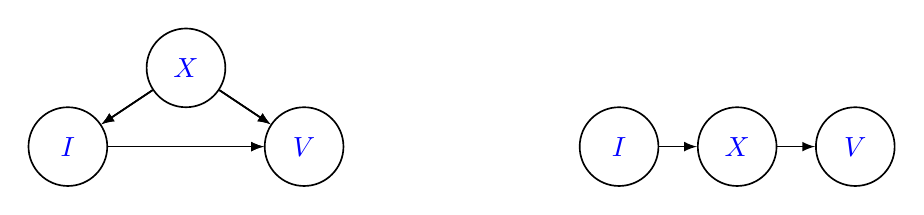
\begin{tikzpicture}[-latex ,auto ,node distance =4 cm and 5cm ,on grid ,
semithick ,
state/.style ={ circle ,top color =white ,
draw , text=blue , minimum width =1 cm}]
\node[state] (B) [right] {$V$};
\node[state] (A) [left = 3cm of B] {$I$};
\node[state] (C) [above right = 1cm and 1.5cm of A] {$X$};
\path (A) edge [] node[above] {} (B);
\draw (C) -- (A);
\draw (C) -- (B);
\node[state] (D) [right = 4cm of B] {$I$};
\node[state] (E) [right = 1.5cm of D] {$X$};
\node[state] (F) [right = 1.5cm of E] {$V$};
\path (A) edge [] node[above] {} (B);
\draw (C) -- (A);
\draw (C) -- (B);
\draw (D) -- (E);
\draw (E) -- (F);
\end{tikzpicture}
\end{center}


In the first case,
\begin{align}
    P(V|\phi)&=\sum_{I,X} P(X) P(I|X,\phi) P(V|I,X,\phi)\\
             &=\sum_{I,X} \phi(X)(I) P(X)  P(V|I,X,\phi_{obs}) \label{eq:hc_xcov}
\end{align}
while in the second case
\begin{align}
    P(V|\phi)&=\sum_I P(I|\phi) P(V|I,\phi) \\
             &=\sum_I \phi(\varnothing)(I) P(V|I,\phi_{obs})\\
             &=\sum_{I,X} \phi(\varnothing)(I) P(X|I,\phi_{obs}) P(V|I,X,\phi_{obs}) \label{eq:int_xcov}
\end{align}
Equations \ref{eq:hc_xcov} and \ref{eq:int_xcov} are not in general equal.

\subsubsection{Causal Bayesian Networks}

For Causal Bayesian Networks, we will identify the intervention $do(I=i)$ with the constant policy $\pi_i$.

For some graph $G$ and some node $I$, denote the graph deleting all outgoing edges of $I$ by $G_{\underline{I}}$ and the graph obtained by deleting all incoming edges to $I$ as $G_{\overline{I}}$.

Assume that with respect to some graph $G$, $P$ satisfies the conditions of a Causal Bayesian Network (Definition \ref{def:CBN}) for $P(V|do(I=i)=P(V|\pi_i)$, $\forall i\in I$. Given this assumption, a key criterion for identifiability in Causal Bayesian Networks is the ``back-door'' criterion:

If $X\subset A$ are observed, then $I\perp_{G_{\underline{I}}} V|X$

There is also a ``front-door'' criterion, which depends on a more complex graph structure.

The back-door criterion implies ignorability \cite{pearl_causality:_2009}. Furthermore, a CBN does not suffer from the covariate adjustment ambiguity above.

The common support assumption doesn't seem to be mentioned much in the CBN literature, but it is also required for identifiability as it has been defined in \ref{def:causal_ident}. In particular, it may not be possible to identify the effects of all policies of interest. It's easy to verify that the probability distribution generated by $\Phi=\pi_1$, $V=I$ satisfies the above conditions for the graph

\begin{center}
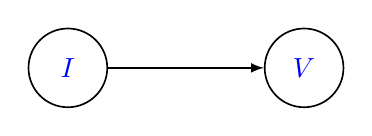
\begin{tikzpicture}[-latex ,auto ,node distance =4 cm and 5cm ,on grid ,
semithick ,
state/.style ={ circle ,top color =white ,
draw , text=blue , minimum width =1 cm}]
\node[state] (B) [right] {$V$};
\node[state] (A) [left = 3cm of B] {$I$};
\path (A) edge [] node[above] {} (B);
\end{tikzpicture}
\end{center}

However, this doesn't allow for $P(V|\pi_0)$ to be consistently estimated - $P(V|I=0,\Phi=\pi_1)$ asks us to condition on a contradiction.

It is straightforward to define a distribution under a conditional intervention using a CBN: $P(V|\Phi=\phi)=\sum_X P(V|X,\Phi=\phi(x)) P(X)$. This amounts to a modification of Definition \ref{def:CBN} where we extend the parental adjustment assumption to cover $do$ interventions with arguments that may depend on other nodes in the graph. There are reasonable situations in which this extension may not hold, even if the original assumption holds (see section \ref{sssec:SUTVA} below).

\subsubsection{Untestability of key assumptions}

Given the ``one-kernel'' rule, we are restricted to knowing at most one of $P(V|X=x,\Phi=\phi,I=0)$ and $P(V|X=x, I=0, \Phi=\phi_{obs})$ if $\phi\neq \phi_{obs}$. Thus, we cannot in general test whether these distributions are equal, as the ignorability assumption asserts. 

Furthermore, it is may not be intuitively obvious when the assumption holds. A common practical approach is to make $X$ a very large set of covariates. It is not obvious when $X$ is a large enough set of covariates, nor is it obvious if the covariates included should be adjusted for (as in the first example above) or not adjusted for (as in the second).

The back-door criterion is also untestable for general $\phi_{obs}$. No property of the distribution $P(V,I,X)$ can rule out the existence of some unmeasured $X'$ such that $X'$ is a common ancestor of $V$ and $I$, which would create an additional back-door path.

I also propose a pair of assumptions that entail both ignorability and the back-door criterion. Like the potential outcomes approach, they allow for causal effects to be defined without assuming that the full set of random variables can be modeled as a CBN. Unlike the potential outcomes approach, these assumptions are not ambiguous over how to adjust for covariates. They are sufficient and not necessary conditions:

\begin{enumerate}
    \item Known domain: Every $\phi\in\Phi\cup \Phi_T$ has domain $A$, and $A$ is observed
    \item Policy is not intrinsically relevant: $P(V|A,I,\Phi)=P(V|A,I)$ for all $a\in A$, $i\in I$, $\phi\in \Phi$
\end{enumerate}

\subsubsection{Interactions}\label{sssec:SUTVA}

A challenge for the CBN framework of causal inference is situations where the effects of separate intervention decisions may interact.

Suppose a vaccine for a contagious disease is being tested on two individuals who live in the same home. The probability of infection $D$ depends on both the vaccination decision $V$ and the presence of another infected person $P$:

\begin{table}[]
    \centering
    \begin{tabular}{c|c|c}
        & $P=0$ & $P=1$ \\
         \hline
        $V=0$ & 0.5 & 1 \\
        $V=1$ & 0.2 & 0.4
    \end{tabular}
    \caption{Probability of disease $D$ by vaccination and presence of infection}
    \label{tab:vaccination_interaction}
\end{table}

For simplicity's sake, we will posit there are two opportunities for infection, both governed by the probabilities in the above table. At the first infection opportunity, neither housemate is infected. However, the presence of infection is only measured once, at the end of the second period.

If the decision to vaccinate $\Phi$ has domain $\varnothing$, we could naively model the situation with the following graph for each individual:

\begin{center}
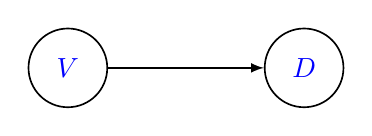
\begin{tikzpicture}[-latex ,auto ,node distance =4 cm and 5cm ,on grid ,
semithick ,
state/.style ={ circle ,top color =white ,
draw , text=blue , minimum width =1 cm}]
\node[state] (A) [left] {$V$};
\node[state] (B) [right = 3cm of A] {$D$};
\path (A) edge [] node[above] {} (B);
\end{tikzpicture}
\end{center}

If $\Phi$ is restricted to constant policies $\pi_0:V\mapsto 0$ and $\pi_1:V\mapsto 1$, the parental adjustment condition must hold for the above graph, as $V=0\implies \phi=\pi_0$ and so $P(D|V=0)=P(D|\Phi=\pi_0)$. However, this is not true for general policies. If the unobserved housemate is vaccinated, then we have
\begin{align}
    P(D|V=0) &= 0.5 + (1-0.5)(0.2*0.5+0.4*1) \\
             &= 0.75 \\
    P(D|\Phi=\pi_0) &= 0.5 + (1-0.5)(0.5*0.5 + 0.5*1) \\
            &= 0.875 \\
            &\neq P(D|V=0)
\end{align}

Another naive attempt would fail due to containing a cycle. Here $V^i$ ($D^i$) are the vaccination (infection) states of the $i$th housemate:

\begin{center}
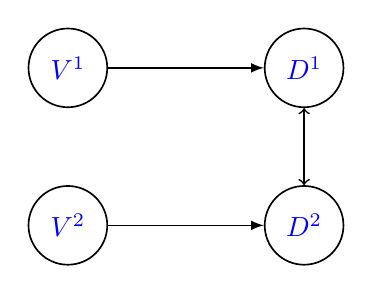
\begin{tikzpicture}[-latex ,auto ,node distance =4 cm and 5cm ,on grid ,
semithick ,
state/.style ={ circle ,top color =white ,
draw , text=blue , minimum width =1 cm}]
\node[state] (A) [left] {$V^1$};
\node[state] (D) [below = 2cm of A] {$V^2$};
\node[state] (B) [right = 3cm of A] {$D^1$};
\node[state] (C) [right = 3cm of D] {$D^2$};
\draw (A) -- (B);
\draw (D) -- (C);
\draw[<->] (B) -- (C);
\end{tikzpicture}
\end{center}

A working CBN model is possible, but it demands modelling the dynamics of the system which may introduce many degrees of freedom and not always be necessary. Here $D^1_i$ is the infection state of housemate 1 at time $i$:

\begin{center}
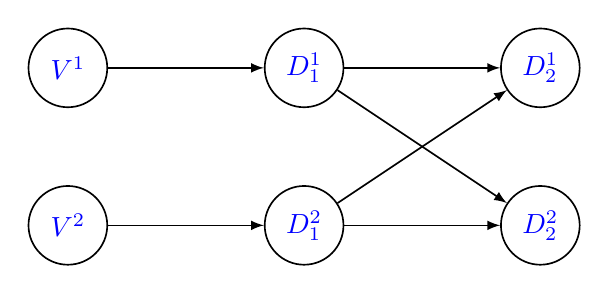
\begin{tikzpicture}[-latex ,auto ,node distance =4 cm and 5cm ,on grid ,
semithick ,
state/.style ={ circle ,top color =white ,
draw , text=blue , minimum width =1 cm}]
\node[state] (A) [left] {$V^1$};
\node[state] (F) [below = 2cm of A] {$V^2$};
\node[state] (B) [right = 3cm of A] {$D^1_1$};
\node[state] (C) [right = 3cm of F] {$D^2_1$};
\node[state] (D) [right = 3cm of B] {$D^1_2$};
\node[state] (E) [right = 3cm of C] {$D^2_2$};
\draw (A) -- (B);
\draw (F) -- (C);
\draw (B) -- (E);
\draw (C) -- (D);
\draw (B) -- (D);
\draw (C) -- (E);
\end{tikzpicture}
\end{center}

The assumption that these kind of interactions don't occur is discussed in the Potential Outcomes literature as part of the "stable unit treatment value assumption" (SUTVA).

\textbf{Question: } How does the ``policy-intrinsic-irrelevance'' assumption behave when there might be interactions of this form?




% \begin{definition}[Interventional projection]
% Define an equivalence relation $\sim$ on $A$ such that $a\sim a'$ iff $P(V|a,i)=P(V|a',i)$ for all $i\in I$. Denote by $E_a$ the equivalence class of $a\in A$ induced by $\sim$, and $\mathbf{E}_A$ the set of such equivalence classes. The interventional projection of $A$ is the map $g:A\to\mathbf{E}_A$. 
% \end{definition}

% \begin{definition}[Complete interventional projection]
% An interventional projection is complete with respect to a policy $f$ if for every $i\in I$ and $E_a\in\mathbf{E}_A$ there exists $a\in E_a$ such that $f(a)=i$.
% \end{definition}

% \begin{example}[Complete interventional projection]
% Suppose $A=X\times M$ where $X$ is a set of observed covariates and $M$ is a noise where $V\CI M | I$. Then $g(x,\mu)=x$ is an interventional projection of $A$, and for any $f$ where for all $i,x$ there exists a $\mu\in M$ such that $f(x,\mu)=i$, $g$ is a complete interventional projection.
% \end{example}

% \begin{theorem}[Complete interventional projection implies policy identifiability]
% Given a causal optimisation problem $\langle P, V, \mathcal{F}, I, A, \mathcal{C}\rangle$, if there is some $f\in\mathcal{F}$ such that there is a complete interventional projection $g:A\to\mathbf{E}_A$, then $P$ is identifiable.
% \end{theorem}

% \begin{proof}
% Take $f\in\mathcal{F}$ to be a policy with a complete interventional projection $g$. Given arbitrary $a\in A$ and $i\in I$, we have $P(V|a,i)=P(V|a',i)$ for any $a'\in g(a)$. By assumption, there exists some $a'\in g(a)$ such that $f(a')=i$, and so $P(V|a',i)$ can be consistently estimated.
% \end{proof}




% \subsection{Recovering a model-selection rule}

% Given $f:X\to \mathbb{R}$, define $\text{argmin}_x f(x) = \{x: f(x)\leq f(x')\text{ for all }x'\in X\}$ (this is the standard definition, I just put it here to emphasise that argmin is a set).

% Suppose we have a loss $L_{M^*,C}:\mathcal{M}\to \mathbb{R}$  and a set of models $\mathcal{M}$ with the property that 
% \begin{align}
%     M \in \mathrm{argmin}_M L_{M^*,C}(M)\implies \mathrm{argmin}_I \mathbb{E}_{M(I)}[C(X)] = \mathrm{argmin}_I \mathbb{E}_{M^*(I)}[C(X)] \label{eq:cq_loss1}
% \end{align}
% Then proceed as in Def. \ref{def:causal_query_1} with $D$ replaced by $M^*$.

% Condition \ref{eq:cq_loss1} is too weak - could strengthen it to for every $\epsilon > 0$ there is $\delta > 0$ s.t.
% \begin{align}
%     M \in \{M:L_{M^*,C}(M) < \mathrm{min}_{M'} L_{M^*,C}(M') + \delta \}\implies \mathrm{argmin}_I \mathbb{E}_{M(I)}[C(X)] = \mathrm{argmin}_I \mathbb{E}_{M^*(I)}[C(X)] + \epsilon \label{eq:cq_loss2}
% \end{align}

% Additional complication: given $\mathcal{S}$, we may not be able to find an approximately optimal model $M$. In particular, we may not be able to bound $|L_{M^*,C}(M)-L_{\mathcal{S},C}(M)|$. ($L_{\mathcal{S}}$ needs definition here).

% \textbf{Are there alternative weaker conditions that may be desirable? Do these lead to actually-existing types of causal inference query?}

% It seems like the two things that might be desirable are, informally, policy improvement and sample complexity improvement. 

% \textbf{Weak policy improvement:} given some prior $P_\mathcal{M}$ over $M$ and $P_\mathcal{M'}$ over $M'=\text{argmin}_M L_{\mathcal{S},C}(M)$ and 
% \[I\in \mathrm{argmin}_I \mathbb{E}_{P_{M}}\left[\mathbb{E}_{M^*(I)}[C(X)]\right]\] \[I'\in \mathrm{argmin}_I \mathbb{E}_{P_{M'}}\left[\mathbb{E}_{M(I)}[C(X)]\right]\]
% weak policy improvement:
% \begin{align}
%     \mathbb{E}_{M^*(I')}[C(X)] < \mathbb{E}_{M^*(I)}[C(X)]
% \end{align}
% Note: introducing $P_\mathcal{M}$ and $P_\mathcal{M'}$ suggests replacing the loss $L$ with Bayes rule?

% \textbf{Sample complexity improvement:} suppose we have $L$ such that Eq \ref{eq:cq_loss2} holds, and there exist extra observations $\mathcal{S}_0$ such that for model class $\mathcal{M}$ w.p. $1-\delta$ we have \[|L_{M^*,C}(M)-L_{\mathcal{S}\cup\mathcal{S}_0,C}(M)|<\epsilon\]

% Suppose we have a loss $\tilde{L}_{\mathcal{S},C}$ such that for $\mathcal{M}'=\mathrm{argmin}_M L_{\mathcal{S},C}(M)$ there exist extra observations $\mathcal{S}_0'$ such that $|\mathcal{S}_0'|<|\mathcal{S}_0|$ and
% \[|L_{M^*,C}(M)-L_{\mathcal{S}\cup\mathcal{S}'_0,C}(M)|<\epsilon\]

% ** This needs a universal quantifier.

% \subsection{Inferring a causal model}

% Given data $D$ over variables $\mathbf{V}$, a class of possible causal models $\mathcal{M}$ and a $D$-dependent loss $\mathcal{L}_D:\mathcal{M}\to \mathbb{R}$, which models $M\subset \mathcal{M}$ minimise $\mathcal{L}_D$?

% Examples: Pearl, chapter 2 \cite{pearl_causality:_2009} - uses estimated distribution $\hat{P}$ rather than data $D$. Proposes two algorithms $IC$ and $IC^*$. Both output sets of CBNs with common conditional independence properties.

% $IC$ considers the class $\mathcal{M}\subset\text{CBN}$ which is the union of all causal structures that can be represented as graphs with exactly one node for each $V\in\mathbf{V}$.

% $IC^*$ considers the class that is the union of all causal structures that can be represented as graphs with one node for each $V\in\mathbf{V}$ and one common cause node for each pair of variables.


% \subsection{Predicting the effect of an intervention}

% Given data $D$ over variables $\mathbf{V}$ and intervention space $\mathcal{I}$, outcome variables $\mathbf{Y}\subset\mathbf{V}$ predictor $\hat{M}:\mathcal{I}\to\text{Range}(Y)$ and loss $\mathcal{L}_D:\hat{M}\to\mathbb{R}$, find $\hat{M}$ minimising $\mathcal{L}_D$.*

% What if we want the complete distribution over $Y$ rather than a point estimate?

%  
\section{Key Questions}

\section{Causal Models}

\subsubsection{Definition of Causal Models}

\begin{definition}[Causal Models]\label{def:causal_models}
Given a set $\mathbf{V}$ of random variables and a set $\mathcal{I}$ of interventions, a causal model is a map $M:\mathcal{I}\to \mathcal{P}(\mathbf{V})$ where $\mathcal{P}(\mathbf{V})$ represents the set of all probability distributions over $\mathbf{V}$.
\end{definition}

\begin{question}
    Do the major examples of causal models in the literature satisfy Definition \ref{def:causal_models}?
    \begin{itemize}
        \item Causal Bayesian Networks
        \item Structural Causal Models
        \item Potential Outcomes/Rubin Causal Model
        \item Marginal models
    \end{itemize}
\end{question}

\subsubsection{Relationships between types of causal models}

\begin{question}
    Are Causal Bayesian Networks equivalent to Structural Causal Models, or is the latter a subset of the former?
\end{question}

\begin{question}
    One feature of structural causal models is the possibility to derive deterministic maps by substituting constants for the noise variables $u_i$. This could be seen as a generalisation of interventions from operations that replace the right hand side of an assignment with a constant to an operation that makes a more general modification to the right hand side of an assignment.
    
    What is the set of general interventions on an SCM that preserve the Markovian property?
\end{question}

\begin{question}
    The basic Rubin Causal Model appears to be a general causal model as in Definition \ref{def:causal_models} with a binary intervention space $\mathcal{I}$ \cite{sontag_causal_nodate}. 
    
    In practice, the Rubin Causal Model is usually used with the assumptions of strong ignorability and stable unit treatment value. Are Rubin Causal Models that satisfy these assumptions also Causal Bayesian Networks?
\end{question}

\subsubsection{Causal models vs probability distributions}

\begin{question}
    Pearl claims there are fundamental differences between causal and probabilistic models \cite{pearl_causality:_2009}. The difference between a causal model in Definition \ref{def:causal_models} and a probability distribution is that a causal model requires the specification of an intervention or distribution over interventions in order to produce a probability distribution over observables. Is this difference sufficient to explain Pearl's dichotomy?
\end{question}

\subsubsection{Causal models vs other kinds of models}

\begin{question}
    What is the relationship between general/Markovian causal models and other system models, particularly where interaction with the system is important? 
    
    Relationship could mean: does one type of model a subset of another? Is there some operation that generates one type of model given another?
    \begin{itemize}
        \item First order state space models
        \item Markov Decision Processes
    \end{itemize}
\end{question}

\subsubsection{Markovian causal models}

\begin{question}
    Is there an appropriate way to define an "approximately Markovian" causal model?
    Points to consider:
    \begin{itemize}
        \item Are there operations we can perform on data generated by a Markovian system that will yield an approximately Markovian system? Example operations: forgetting data for some variables, averaging data over time or over repeated instances.
        \item Is there a "mathematically neat" way to define approximate Markovianity?
    \end{itemize}
\end{question}

\subsection{Causal Inference Problems}

\begin{question}\label{q:causal_queries}
    What are the key kinds of causal queries? A very preliminary list:
    \begin{itemize}
        \item Control/prediction: how would a system behave if intervention $I$ were applied?
        \item Attribution: what is responsible for the observation of outcome $v$?
        \item Latent variables: identifying latent variables causally responsible for observed data
        \item Causal structure: identifying how observed variables are causally related to one another
    \end{itemize}
\end{question}

\begin{question}
    Detecting latent variables has a clear connection to dimensionality reduction \cite{kummerfeld_causal_2016}. As a general question, how does \emph{causal} latent variable detection differ from other forms of dimension reduction?
    
    As a more specific question, is there a particular form of loss function that is, implicitly or explicitly, assumed in causal latent variable detection? 
\end{question}

\begin{question}\label{q:causal_query_difficulty}
    How should the difficulty of a causal query be measured?
    Some possibilities:
    \begin{itemize}
        \item Observational sample complexity
        \item Interventional sample complexity
    \end{itemize}
\end{question}

\begin{question}
    Is it possible to define a generic set of elements that constitute a causal inference query? For example, a control query might require:
    \begin{itemize}
        \item Outcome/objective
        \item Set of allowed interventions
        \item Set of observations
        \item Hypothesis class
        \item Assumptions
        \item Data
    \end{itemize}
\end{question}

\begin{question}
    Causal queries typically employ assumptions over and above the assumptions made for statistical queries. Are additional assumptions always necessary?
    
    More precisely: given a causal model $M$ for which the class $\mathcal{P}$ of distributions satisfies statistical learnability assumptions (clarification pending), what characterises causal queries that are unresolvable without further assumptions?
\end{question}

\begin{question}\label{q:query_set_of_models}
    Given a causal query (pending definition) and the assumption of a Markovian causal model, does the query induce equivalence classes of causal models? Does this depend on the type of query?
\end{question}

\begin{question}
    Can two identical causal models (Definition \ref{def:causal_models}) with different side information (definition pending) give different answers to a causal query (definition pending)?
\end{question}

\begin{question}
    What are key features in a taxonomy of causal inference problems that aims to group problems by which approaches to solving the problem may/may not work? Do the objects identified in Definition \ref{def:causal_models} - $\mathbf{V}$, $\mathcal{I}$, $\mathcal{P}$ play important roles in such a taxonomy?
\end{question}

\begin{question}
    Given a causal bayesian network $M$ with targets $Y$, other observables $X$ and interventions $\mathcal{I}$ and cost $C:\mathcal{I}\times Y\to\mathbb{R}$, are there control strategies possible with $M$ that may be superior to control strategies possible if only $P(Y|I)$ is known for all $I\in\mathcal{I}$?
\end{question}

\subsection{Causal Discovery}

Causal discovery describes any method of learning a set of Markovian causal models that might describe the causal relationships between variables in a dataset.

\begin{question}
    Is it correct to consider queries about causal structures instrumental queries in service of other aims? Alternatively, should causal structures be added to the list in Question \ref{q:causal_queries}?
\end{question}

Many algorithms for causal structure discovery do not resolve whether $X$ and $Y$ are confounded by an unobserved $Z$ or not. On the other hand, the answer many conceivable causal queries will depend on whether two variables are confounded or directly causally related. The next questions focus on whether structural identification can help with causal queries.

\begin{question}\label{q:discovery_set_of_models}
    A structure discovery algorithm will typically output some class $\mathcal{C}$ of causal models. In some cases these classes are well-defined, for example Markov Equivalence Classes. In some cases it is not so clear - algorithms that cannot detect latent confounders are usually introduced with the assumption that no such confounders exist. However, it is also possible to view them as outputting a large class of causal models that contains many models with latent confounders and some without.
    
    The question here is what classes of causal models are output by the various structure learning algorithms?
\end{question}

\begin{question}
    Considering the model sets in \ref{q:query_set_of_models} and \ref{q:discovery_set_of_models}, when is it possible for the output of a structure discovery algorithm to facilitate answering a causal query - for example, by reducing the query to one that is easier on a metric of difficulty (question \ref{q:causal_query_difficulty}).
\end{question}

\begin{question}
    Which causal discovery algorithms require the assumption of faithfulness?
    \begin{itemize}
        \item PC and IC definitely do
        \item Bayesian score based (e.g. Greedy Equivalence Search) I'm not sure
        \item Additive noise models, information geometric definitely don't
        \item Latent factor detection (BPC, FOFC) - I'm not sure \cite{kummerfeld_causal_2016}
    \end{itemize}
\end{question}

\begin{question}
    What is the relationship between $\lambda$ in $\lambda$-faithfulness and sample complexity of PC-type algorithms?
\end{question}

\begin{question}
    Are there weakenings of faithfulness or $\lambda$-faithfulness, and do these allow for consistency results of their own?
    \begin{itemize}
        \item Some types of faithfulness violations have testable implications, so only some types of faithfulness need to be assumed \cite{ramsey_adjacency-faithfulness_2012}
        \item Some types of faithfulness violations could be benign (e.g. violated faithfulness in $X\to Y$) \cite{peters_structural_2013}
        \item The degree to which faithfulness violations impact the answer to a causal query might scale with the number of "non-transparent" conditional independences 
    \end{itemize}
\end{question}

\begin{question}\label{q:volume_unfaithful}
    Is it possible to lower bound the volume of unfaithful distributions for a set of probability distributions $\mathcal{P}_G$ with parametrisation $\mathbf{a}_G$ that are Markovian to an arbitrary graph $G$? \cite{uhler_geometry_2013}
\end{question}

\begin{question}
    Can entropy-based constraints simplify the analysis of sets of faithful distributions in Question \ref{q:volume_unfaithful} (I don't presently understand what entropy-based constraints are, so this question might make no sense. I just recall a comment that entropy based constraints can be easier to work with than geometry of algebraic varieties).
\end{question}

Both the faithfulness assumption and additive noise model causal discovery identify a "contrast function" $C(P):\mathcal{P}\to\mathbb{R}$ of a probability distribution $P$ that, given a measure $\mu_G$ over $\mathcal{P}$ for each CBN $G$, takes generic values for to some CBNs $\mathcal{G}^*$ and nongeneric values for all others $\mathcal{G}^{*C}$. That is, $\mu_{G^*}(C(P))>0$, and $\mu_{G'}(C(P))=0$ for any $G'\in\mathcal{G}^{*C}$.

\begin{question}\label{q:generalised_genericity}
    These genericity conditions hold for a general class of measures $\mu_G$ - for example, if a distribution $P$ is parametrised by $\{a_i\}$ for a graph $G$, then the genericity conditions might hold for any continuous prior over $\{a_i\}$.
    
    However, to get uniform consistency results, we need to allow for some slack around the value of $C(P)$, and consequently need to shift from "non-transparent" probability distributions having measure 0 under $\mu_G$ to having small measure under $\mu_G$.
    
    For what class of measures can we conclude from $\mu_G(C(P)=c_0)=0$ and $|C(\hat{P})-c_0|<\delta$ that $\mu_G(C(\hat{P})\in B_\delta (c_0)) < \epsilon$? Does this depend strongly on $C$?
    
    $B_\delta(x)$ is a ball of radius $\delta$ around $x$.
\end{question}
    
\begin{question}
    Are there any general properties that contrast functions must satisfy?
\end{question}

\begin{question}
    Is there a method to generate contrasts $C$? See \cite{besserve_group_2017} for a discussion of using group transformations for generating measures $\mu_G$.
\end{question}


% 
% A proposed general framework for decision-theoretic causal queries:

% % \begin{definition}[Causal model query]\label{def:causal_query_1}
% % Given complete dataset $D$ over domain $V$ and a sample $S\subset D$, a class of causal models $\mathcal{M}$ and a $D$-dependent loss $\mathcal{L}_D:\mathcal{M}\to \mathbb{R}$, using the sample $S$ find a model $M\in \mathcal{M}$ minimising $\mathcal{L}_D$?
% % \end{definition}

% % Thinking aloud: given a distinction between intervention and other variables $V=X\times \mathcal{I}$, the causal model defined in \ref{def:causal_models} explicitly avoids requiring a marginal distribution $P(\mathcal{I})$, though the conditional $P(X|\mathcal{I}=I)=M(I)$ exists.

% % On the other hand, given a complete dataset $D$, $P(\mathcal{I})$ will exist and $\mathcal{L}_D$ will depend on it. It seems undesirable for a causal query to depend on the selection of intervention.

% % Try stepping up a level of generality:

% % Let $\mathcal{I}$ be an arbitrary set of interventions. If we imagine a robot interacting with the world, we can think of $\mathcal{I}$ as the set of all possible signals the robot could send to its actuators. We will later discuss when it makes sense to consider particular types of intervention such as $do$-type interventions.

% Define the collection of conditionals $P(X|\mathcal{I})=\{P(X|I)|I\in\mathcal{I}\}$.

% \begin{definition}[Causal policy]\label{def:causal_query_2}
% Given a set of conditionals $P(X|\mathcal{I})$ with domain $X$ and interventions $\mathcal{I}$ and a cost function $C:X\times\mathcal{I}\to\mathbb{R}$ find $I$ minimising $\mathbb{E}_{P(X|I)}[C(X,I)]$. The resulting $I$ is the \emph{causal policy}
% \end{definition}

% \subsection{Problems with causal policies}\label{ssec:prob_causal_policy}

% A causal policy (Def \ref{def:causal_query_2}) suggests the existence of an agent with an ability to conduct the interventions $\mathcal{I}$. However, definitions so far leave open the mechanism by which the agent can conduct such interventions. This is undesirable, as if the agent implements a policy using some mechanism $\mu_I$ to conduct intervention $I$, we might justifiably be concerned about whether $P(X|I,\mu_I)=P(X|I)$. This isn't just a theoretical concern - it is easy to come up with examples of situations where $P(X|I,do(I))\neq P(X|I,\neg do(I))$. If we add a node representing $\mu_I$ to the model, we might shift our concern to a potential metamechanism $\mu'_I$ and so forth. It might be intuitively obvious in many cases that we can stop when we reach a given level, but the lack of a formal account is unsatisfying.

% \begin{definition}[Causal optimization problem]\label{def:copt_prob}
% A causal optimization problem is a tuple $\langle \mathcal{I}, V, \mathcal{F}, m, C\rangle$. $V$ is a set of variables and $\mathcal{I}$ is a set of interventions and $V$ is a set of random variables. $\mathcal{F}$ is a set of functions $V\to \mathcal{I}$ and $m$ is a map $\mathcal{F}\to \mathcal{P}_{V\times \mathcal{I}}$, where $\mathcal{P}_{V\times \mathcal{I}}$ is a set of probability distributions on $V\times \mathcal{I}$. $C:V\times \mathcal{I} \to \mathbb{R}$ is a cost function.
% \end{definition}

% \subsection{Functional policy}

% My proposed solution is to incorporate a policy function into the world model. This demystifies what exactly "interventions" are - they are policy function outputs.

% \begin{definition}[Functional policy]\label{def:fp_cpq}
% Suppose we have a domain $X\times\mathcal{I}$, a set of candidate policies $\mathcal{F}:\{X\to \mathcal{I}\}$, a map $m:\mathcal{F}\to \mathcal{P}$ where $\mathcal{P}$ is the space of probability distributions over $X\times\mathcal{I}$ and a cost function $C:X\times\mathcal{I}\to \mathbb{R}$.

% The functional policy is
% \begin{align}
%     \Pi=\mathrm{argmin}_{f\in\mathcal{F}}\mathbb{E}_{m(f)}[C(x,I)]    \label{eq:func_cp}
% \end{align}
% \end{definition}

% As the codomain of the map $m$ is a space of probability distributions, I will use the notation
% \begin{align}
%     P_\Pi := m(\Pi)
% \end{align}

% Needs work: I think that the domain of functions in $\mathcal{F}$ should probably be restricted to things that happen before the function is computed. I'm reluctant to include time if it can be avoided, so leaving it as a note for now.

% Definition \ref{def:fp_cpq} is motivated by the following consideration: Suppose we have a true set of conditionals $P^*(X|\mathcal{I})=\{P^*(X|I):\forall I \in \mathcal{I}\}$. Deducing a policy from \ref{def:causal_query_2} using the model $P(X|\mathcal{I})=P^*(X|\mathcal{I})$ is not sufficient to ensure the chosen policy is actually optimal because we haven't specified a model of how the agent interacts with $\mathcal{I}$. Suppose, instead, we have a map $m^*:\mathcal{F}\to\mathcal{P}$ that is true for all $f\in\mathcal{F}$ and derive an optimal policy $\Pi\in\mathcal{F}$ following \ref{def:fp_cpq} with $m=m^*$. This is sufficient to ensure that $\Pi$ is superior to all other policies in $\mathcal{F}$.

% % \begin{remark}
% % If the set of distributions $\mathcal{P}$ are able to be represented by structural equation models, all variables are functions of other variables in the model. Intervention variables are then distinguished only by the freedom to choose which function computes them.
% % \end{remark}


% \subsubsection{Self-optimisation}\label{sssec:self_reflection}

% Finding an optimal policy via Definition \ref{def:fp_cpq} is itself the application of a map $Q:\{\mathcal{F}\}\times\{\mathcal{F}\to\mathcal{P}\}\times\{\mathcal{I}\to\mathbb{R}\}\to\{X\to\mathcal{I}\}$ such that $Q(\mathcal{F},m,C)=\Pi$ (with symbols defined as above). 

% Introducing a map $G\{X\to X\to \mathcal{I}\} \to \{X\to\mathcal{I}\}$, $G(Q)$ is itself a policy - in fact it is the policy actually implemented by the agent, while the idealised $\Pi:=Q(X)$ will, in general, forget some of the inputs of $G(Q)$. 

% It is interesting to ask whether it is possible to set the optimisation problem up so that $\Pi=G(Q)$, and what implications this might have. To do so, we must ensure that $G(Q)\in\mathcal{F}$, and so we must augment the domain $X$ with variables representing $\mathcal{F}$,$m$ and $C$.

% Needs work: the fact that the model $m$ must contain a representation of itself is suggestive of an incomputability result. Is there such a result here?

% Needs work: Generally, when is it possible to take a policy $\Pi_1:X\to\mathcal{I}$ and produce a simplified policy $\Pi_2:C\to\mathcal{I}$ where $C\subset X$ which achieves the same cost?


% \subsection{Functional policies in Bayesian Networks}

% The definitions above do not require the probability distributions $\mathcal{P}$ be Markovian. However, Markovian distributions permit easy representation of conditional independence with graphical models, so they make a good basis from which to generate examples.

% We will follow the custom of labeling nodes in a graphical model with the output of the function represented by the node, so the policy node will be labeled $I$.

% We will also neglect any subtleties raised by section \ref{sssec:self_reflection}.

% Needs work: the inclusion of a policy function suggests that $I$ may be locally Markovian with respect to the inputs to the policy function. Need to check the exact characteristics WRT Markovianity.

% \subsubsection{Simple case}\label{sssec:simple_case}

% Let $\mathcal{I},X=\{0,1\}$ and $C(x,I)=x$.

% \begin{center}
% \begin{tikzpicture}[-latex ,auto ,node distance =4 cm and 5cm ,on grid ,
% semithick ,
% state/.style ={ circle ,top color =white ,
% draw , text=blue , minimum width =1 cm}]
% \node[state] (A) [left] {$I$};
% \node[state] (B) [right = of A] {$X$};
% \path (A) edge [] node[above] {} (B);
% \end{tikzpicture}
% \end{center}

% We will partially define the probability distribution with the following structural equation:
% \begin{align*}
%     X:=I
% \end{align*}
% Choosing a function that computes $I$ will complete the definition.

% Given the dependences indicated, we have as $\mathcal{F}$ the set of constant functions on $\mathcal{I}$. Of these, $I\mapsto0$ minimises $C$.

% In this simple case, finding the functional policy reduces to finding the best intervention. 

% \subsubsection{Additional dependence}

% Let $\mathcal{I},X_1,X_2=\{0,1\}$ and $C(x_1,x_2,I)=x_1$. Suppose $X_2$ is observed before $I$ is computed, so it is a potential input of the policy.

% \begin{center}
% \begin{tikzpicture}[-latex ,auto ,node distance =4 cm and 5cm ,on grid ,
% semithick ,
% state/.style ={ circle ,top color =white ,
% draw , text=blue , minimum width =1 cm}]
% \node[state] (B) [right] {$X_1$};
% \node[state] (A) [above left = 1cm and 3cm of B] {$X_2$};
% \node[state] (C) [below left = 1cm and 3cm of B] {$I$};
% \path (A) edge [] node[above] {} (B);
% \path (C) edge [] node[above] {} (B);
% \draw[dashed] (A) -- (C);
% \end{tikzpicture}
% \end{center}

% We will partially define the distribution with:
% \begin{align*}
%     X_1 := \mathrm{XOR}(I,X_2)
% \end{align*}

% We could consider policies that are constant on $\{0,1\}$, or maps $\{0,1\}\to\{0,1\}$. Clearly in this case we want $\Pi:I\mapsto X_2$. If we further knew that $P(X_2=0)=1$, then the constant policy $f:I\mapsto 0$ would perform equally well.

% \begin{remark}
% The optimal policy isn't straightforward to derive using Causal Bayesian Networks. If we consider the setup above where we are permitted to conduct interventions on the node labeled by $I$, under the standard definition of intervention we would assume that it cuts off any dependence of $I$ on $X_2$. This would limit us to what are here described as constant policies, which are not in general optimal. 

% We could address this by proposing that $do()$-interventions could depend on the value of $X_2$ even if $I$ does not depend on it directly. This would invalidate some properties of Causal Bayesian Networks.
% \end{remark}

% \begin{remark}
% If the policy depends on $X_2$, we never need to know the full probability distribution to find the optimal policy.
% \end{remark}

% \subsubsection{Hidden dependence}
% Let $\mathcal{I},X_1,X_2=\{0,1\}$ and $C(x_1,x_2,I)=x_1$. Suppose $X_2$ is not observed.

% \begin{center}
% \begin{tikzpicture}[-latex ,auto ,node distance =4 cm and 5cm ,on grid ,
% semithick ,
% state/.style ={ circle ,top color =white ,
% draw , text=blue , minimum width =1 cm}]
% \node[state] (B) [right] {$X_1$};
% \node[state,dashed] (A) [above left = 1cm and 3cm of B] {$X_2$};
% \node[state] (C) [below left = 1cm and 3cm of B] {$I$};
% \path (C) edge [] node[above] {} (B);
% \draw[dashed] (A) -- (B);
% \end{tikzpicture}
% \end{center}

% We will assume the following structural equations
% \begin{align*}
%     X_2 &:= \mu_{X_2}\\
%     X_1 &:= \mathrm{XOR}(I,X_2)
% \end{align*}
% Where $\mu_{X_2}\sim \mathrm{Bernoulli}(0.2)$.

% In this case, the problem appears to be identical to a problem with the dependence structure of \ref{sssec:simple_case}, and the optimal policy is constant $\Pi:I\mapsto 1$.

% \subsubsection{Confounded observations}
% Let $\mathcal{I},X_2=\{0,1\}$, $X_1=\{0,1,2\}$ and $C(x_1,x_2,I)=x_1$. Suppose $X_2$ is not observed.

% Suppose also that we make infinite observations under some fixed policy $f$, and we are then free to impose our preferred policy $\Pi$.

% \begin{center}
% \begin{tikzpicture}[-latex ,auto ,node distance =4 cm and 5cm ,on grid ,
% semithick ,
% state/.style ={ circle ,top color =white ,
% draw , text=blue , minimum width =1 cm}]
% \node[state] (B) [right] {$X_1$};
% \node[state,dashed] (A) [above left = 1cm and 3cm of B] {$X_2$};
% \node[state] (C) [below left = 1cm and 3cm of B] {$I$};
% \path (C) edge [] node[above] {} (B);
% \draw[dashed] (A) -- (B);
% \draw (A) -- (C);
% \end{tikzpicture}
% \end{center}

% We will assume the following structural equations
% \begin{align*}
%     X_2 &:= \mu_{X_2}\\
%     X_1 &:= \neg I + X_2 \\
%     f   &:= X_2
% \end{align*}
% Where $\mu_{X_2}\sim \mathrm{Bernoulli}(0.2)$.

% The optimal policy will be $\Pi:I\mapsto 0$, but from our observations it will appear that $X_1 \CI I$ which would suggest that $\Pi$ is no better than the alternative.

% \subsubsection{Randomisation}
% Let $\mathcal{I}\{0,1\}$, $X_1=\{0,1,2\}$, $N=\{0,1,..,i,..,n\}$ and $C(x_1,i,I)=x_1$. Suppose $X_2$ is not observed.

% We wish to estimate the distribution of $X_1$ under fixed policies $f_0:I\mapsto 0$ and $f_1:I\mapsto 1$, and we can sample the system $n$ times. In order to do this, we will in fact be sampling under the policy $r:N\mapsto \{0,1\}$.

% \begin{center}
% \begin{tikzpicture}[-latex ,auto ,node distance =4 cm and 5cm ,on grid ,
% semithick ,
% state/.style ={ circle ,top color =white ,
% draw , text=blue , minimum width =1 cm}]
% \node[state] (B) [right] {$X_1$};
% \node[state,dashed] (A) [above left = 1cm and 3cm of B] {$N$};
% \node[state] (C) [below left = 1cm and 3cm of B] {$I$};
% \path (C) edge [] node[above] {} (B);
% \draw[dashed] (A) -- (B);
% \draw (A) -- (C);
% \end{tikzpicture}
% \end{center}

% The dependence structure is identical to the previous section, which showed that in general it isn't possible to deduce the optimal policy from these observations. The difference is that we are free to choose $r$.

% Suppose there is some set of ``plausible'' functions $\mathcal{H}=\{N\times I\to X_1\}$. If we choose $f'$ such that 
% \begin{align}
%     \max_{h\in\mathcal{H}} \left| \langle \{h(i,0):r(i)=0\}\rangle - \langle \{h(i,0):i\in\{n\}\} \rangle \right| < \epsilon \label{eq:bin_random}
% \end{align}
% Where $\langle\cdot\rangle$ denotes an average. If we suppose this also holds for $h(\cdot,1)$, then we can be confident that the subset of samples for which $r(i)=0$ will provide a good estimate for the distribution of $X_1$ under $f_0$, and the subset for which $r(i)=1$ will provide a good estimate for the distribution under $f_1$.

\subsection{Identifiability}

\subsubsection{Causal Bayesian Networks}

In the Pearlean framework, the causal effect of $X$ on $Y$ is identifiable if $P(y|do(X=i))$ is able to be consistently estimated from infinite observational data for all $i\in \mathrm{Range}(X)$. Given a graph $G$ over vertices $V$ representing a CBN (def \ref{def:CBN}) and a subset $X\subset V$, denote the graph deleting all outgoing edges of $X$ by $G_{\underline{X}}$ and the graph obtained by deleting all incoming edges to $X$ as $G_{\overline{X}}$.

Under these assumptions, four conditions for the identifiability of $X$ on $Y$ are given that are claimed to be both necessary and sufficient. The faithfulness assumption is not mentioned in the reference, but I can provide an example of an identifiable effect where $P$ is minimial but not faithful to $G$ and the following conditions do not hold \cite{galles_testing_2013}. Recall d-separation (definition \ref{def:dsep}) for the points below:

\begin{enumerate}
    \item There is no path from $X$ to $Y$ in $G$
    \item (No back-door path) $X\perp_{G_{\underline{X}}} Y$
    \item (All back-door paths blocked) If $Z\subset V$ are observed, then $X\perp_{G_{\underline{X}}} Y|Z$
    \item (``Front-door'' criterion) There exists $Z_1, Z_2 \subset V$ such that
    \begin{itemize}
        \item $Z_2\cap X =\varnothing$
        \item $Z_1$ blocks all directed paths from $X$ to $Y$: $X \perp_{G_{\overline{X}}} Y | Z_1$
        \item $Z_2$ blocks all back-door paths between $Z_1$ and $Y$ in $G_{\overline{X}}$: $Z_1 \perp_{G_{{\overline{X}}{\underline{Z_1}}}} Y | Z_2$
        \item $Z_2$ blocks all back-door paths between $X$ and $Z_1$: $Z_1 \perp_{G_{{\underline{X}}}} X | Z_2$
    \end{itemize}
\end{enumerate}

Recall that $d$-separation statements imply conditional independences in the associated probability distribution.

\subsubsection{Challenges for the CBN account of identifiability}

\textbf{No assumption of common support} 

It's easy to verify that the probability distribution generated by $P(I=i)=\delta(i)$, $V=I$ is a CBN compatible with the following graph that satisfies condition 2:

\begin{center}
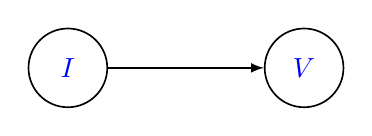
\begin{tikzpicture}[-latex ,auto ,node distance =4 cm and 5cm ,on grid ,
semithick ,
state/.style ={ circle ,top color =white ,
draw , text=blue , minimum width =1 cm}]
\node[state] (B) [right] {$V$};
\node[state] (A) [left = 3cm of B] {$I$};
\path (A) edge [] node[above] {} (B);
\end{tikzpicture}
\end{center}

However, this doesn't allow for $P(V|do(I=1))$ to be estimated, as $I=1$ is inconsistent with the assumed distribution of $I$.

\textbf{Difficulties modelling interactions}

Suppose a vaccine for a contagious disease is being tested on two individuals who live in the same home. The probability of infection $D$ depends on both the vaccination decision $V$ and the presence of another infected person $P$:

\begin{table}[h]
    \centering
    \begin{tabular}{c|c|c}
        & $P=0$ & $P=1$ \\
         \hline
        $V=0$ & 0.5 & 1 \\
        $V=1$ & 0.2 & 0.4
    \end{tabular}
    \caption{Probability of disease $D$ by vaccination and presence of infection}
    \label{tab:vaccination_interaction}
\end{table}

For simplicity's sake, we will posit there are two opportunities for infection, both governed by the probabilities in the above table. At the first infection opportunity, neither housemate is infected. However, the presence of infection is only measured once, at the end of the second period, and individuals don't recover once infected.

If the distribution of $V$ is either $P(V=1)=1$ or $P(V=1)=0$, the following graph could be argued to be a valid CBN for the distribution defined above:

\begin{center}
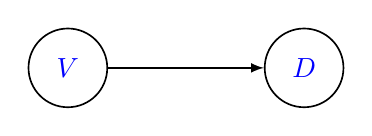
\begin{tikzpicture}[-latex ,auto ,node distance =4 cm and 5cm ,on grid ,
semithick ,
state/.style ={ circle ,top color =white ,
draw , text=blue , minimum width =1 cm}]
\node[state] (A) [left] {$V$};
\node[state] (B) [right = 3cm of A] {$D$};
\path (A) edge [] node[above] {} (B);
\end{tikzpicture}
\end{center}

It is frequently mentioned that the $P(Y|do(X=x))$ should be able to be thought about as the distribution of $Y$ given that $X$ was set to $x$ \emph{by a randomised experiment}, which is not true in this case.

The situation can be correctly modeled with a CBN which captures the dynamics. Modelling the dynamics is necessary to avoid cycles in the causal graph. Here $D^i_j$ is the infection state of housemate $i$ at time $j$:

\begin{center}
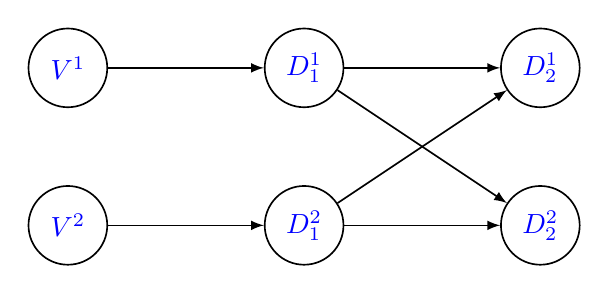
\begin{tikzpicture}[-latex ,auto ,node distance =4 cm and 5cm ,on grid ,
semithick ,
state/.style ={ circle ,top color =white ,
draw , text=blue , minimum width =1 cm}]
\node[state] (A) [left] {$V^1$};
\node[state] (F) [below = 2cm of A] {$V^2$};
\node[state] (B) [right = 3cm of A] {$D^1_1$};
\node[state] (C) [right = 3cm of F] {$D^2_1$};
\node[state] (D) [right = 3cm of B] {$D^1_2$};
\node[state] (E) [right = 3cm of C] {$D^2_2$};
\draw (A) -- (B);
\draw (F) -- (C);
\draw (B) -- (E);
\draw (C) -- (D);
\draw (B) -- (D);
\draw (C) -- (E);
\end{tikzpicture}
\end{center}

However, it seems legitimate to be interested $P(D^1,D^2|V^1,V^2)$, and it is possible to find this without needing to posit a model of the dynamics.

\subsubsection{Potential Outcomes}

The potential outcomes approach employs substantially different terminology to the CBN view of causality. It is specified through a mixture of formal definition and example, and I'm going to reproduce that here because I want to avoid imposing my own ideas about formal definitions on it.

Suppose a randomised trial with two treatment options $T\in\{0,1\}$ is administered to an infinite number of participants. For each participant $i\in\mathbb{N}$ there is a random variable $Y_i$ indicating the outcome of that participant. There are random variables $Y_i(0)$ and $Y_i(1)$ indicating the outcome participant $i$ would have experienced had they not received or received treatment respectively. For each participant there is an extra variable $X_i$ consisting of extra features related to the administration (or not) of the treatment to participant $i$. Finally there is a set of variables $W_i$ indicating the treatment assignment of participant $i$.

Given this setup, the potential outcomes approach often aims to estimate $\langle Y(1) \rangle - \langle Y(0) \rangle$ where $\langle \cdot \rangle$ indicates an average over every participant. 

There are a few assumptions given as necessary to be able to estimate this quantity:

\textbf{Stable unit treatment value assumption}: for any $i$, the values of $Y_i(0)$ and $Y_i(1)$ don't depend on any function of the set of treatment assignments $\{W_i:i\in\mathbb{N}\}$. I'm editorializing here, Rubin puts it this way: "First, it assumes that there is no interference between units (Cox 1958); that is, neither Y i (1) nor Y i (0) is affected by what action any other unit received. Second, it assumes that there are no hidden versions of treatments; no matter how unit i received treatment 1, the outcome that would be observed would be Y i (1) and similarly for treatment 0." 

\textbf{Ignorability}: Define $Y_{obs}(1)=W_i Y_i(1)$ and $Y_{obs}(0)= (1-W_i)Y_i(0)$. Ignorability holds that \begin{align}
    P(Y_i(1)|W_i=1,X_i=x) &= P(Y_i(1)|X_i=x) \\
    P(Y_i(0)|W_i=0,X_i=x) &= P(Y_i(0)|X_i=x)
\end{align}

\textbf{Common support}: Common support is the assumption that for all $w\in \mathrm{Range}(W_i)$, $x\in \mathrm{Range}(X_i)$
\begin{align}
    P(W_i=w|X_i=x) > 0
\end{align}

\subsubsection{Challenges for the Potential Outcomes approach to identifiability}

\textbf{Inaccessibility of the ignorability assumption}

The ignorability assumption can't be tested, as $Y_i(0)$ is not known in every case. This is problematic in particular because there are few cases besides randomised control trials in which a strong argument can be made that it holds.

A typical approach to solving the problem outside of RCTs is to add a large vector of covariates $X$ and hope that this causes ignorability to hold. It's not clear when this might or might not be a sound approach.

\textbf{Ambiguity over how to adjust for $X$}

Consider the following two cases, and assume extended ignorability:

\begin{center}
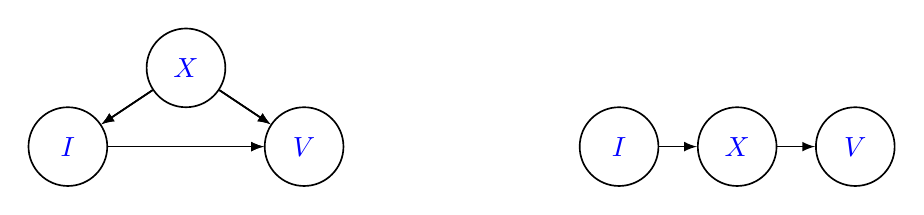
\begin{tikzpicture}[-latex ,auto ,node distance =4 cm and 5cm ,on grid ,
semithick ,
state/.style ={ circle ,top color =white ,
draw , text=blue , minimum width =1 cm}]
\node[state] (B) [right] {$V$};
\node[state] (A) [left = 3cm of B] {$I$};
\node[state] (C) [above right = 1cm and 1.5cm of A] {$X$};
\path (A) edge [] node[above] {} (B);
\draw (C) -- (A);
\draw (C) -- (B);
\node[state] (D) [right = 4cm of B] {$I$};
\node[state] (E) [right = 1.5cm of D] {$X$};
\node[state] (F) [right = 1.5cm of E] {$V$};
\path (A) edge [] node[above] {} (B);
\draw (C) -- (A);
\draw (C) -- (B);
\draw (D) -- (E);
\draw (E) -- (F);
\end{tikzpicture}
\end{center}


In the first case,
\begin{align}
    P(V|\phi)&=\sum_{I,X} P(X) P(I|X,\phi) P(V|I,X,\phi)\\
             &=\sum_{I,X} \phi(X)(I) P(X)  P(V|I,X,\phi_{obs}) \label{eq:hc_xcov}
\end{align}
while in the second case
\begin{align}
    P(V|\phi)&=\sum_I P(I|\phi) P(V|I,\phi) \\
             &=\sum_I \phi(\varnothing)(I) P(V|I,\phi_{obs})\\
             &=\sum_{I,X} \phi(\varnothing)(I) P(X|I,\phi_{obs}) P(V|I,X,\phi_{obs}) \label{eq:int_xcov}
\end{align}
Equations \ref{eq:hc_xcov} and \ref{eq:int_xcov} are not in general equal. Rubin recommends not adjusting for effects of the intervention, but this is somewhat ad-hoc as the potential outcomes approach doesn't actually define what an "effect of an intervention" is \cite{rubin_causal_2005}.

\subsubsection{Policy based identifiability}

Here is working definitions of causal models and causal identification problems:

\begin{definition}[Causal Model]
A causal model is a tuple $\mathcal{M} = \langle V, \Phi, P_\Phi \rangle$. $V$ is a set of variables with subsets $A, I\subset V$, and $\Phi$ is a set of Markov kernels $\phi:A\to \Delta I$. $P_\phi : \Phi\to \Delta V$ is a map from $\Phi$ to distributions on $V$. Even though $\Phi$ is not a random variable, we will write $P(V|\phi) := P_\phi(V)$.
\end{definition}

\begin{definition}[Causal identification problem]\label{def:causal_ident_prob}
A causal identification problem is a problem of  the form: Given a set of variables $V$, policies $\Phi$ and  whose joint dynamics are governed by an unknown causal model $\mathcal{M}$, find $P(V|\phi)$ for each $\phi\in \Phi$.
\end{definition}

The policy $\Phi$ can be understood to be a generalisation of $do(X=x)$ to a ``conditional do''. Under $do(X=x)$ a CBN assigns probability 1 to $X=x$. A Markov kernel $\phi$ can instead assign a range of distributions to $X$ which may depend on other variables.

A Markov kernel $\phi$ with the unit number $i$ in its domain can also be identified with the assignment variable $W_i$ in the potential outcomes approach. 

Under these conditions, it is possible to identify a causal model if three assumptions hold:

\textbf{Policy exchangeabilty}: $P(V\setminus\{A,I\}|A,I,\phi)=P(V\setminus\{A,I\}|A,I,\phi')$ for all $\phi,\phi' \in \Phi$

\textbf{Common support}: There exists a policy $\phi_{obs}\in\Phi$ for which $\phi_{obs}(a,i)>0$ for all $a\in A$, $i\in I$.

\textbf{Domain independence}: For all $\phi\in \Phi$, $P(A|\phi)=P(A|\phi')\overset{\mathrm{def}}{=}P(A)$

Issue: is domain independence necessary?

\begin{proof}
For any $\phi\in\Phi$,
\begin{align}
    P(V|\phi)&=\sum_{a}\sum_{i} P(V|a,i,\phi)\phi(a,i)P(a|\phi) \\
            &= \sum_{a}\sum_{i} P(V|a,i,\phi_{obs})\phi(a,i)P(a)
\end{align}

$P(V|a,i,\phi_{obs})$ and $P(a)$ can be estimated from i.i.d. observations of $V$ under $\phi_{obs}$ and $\phi(a,i)$ is known.

\end{proof}

The difference between this approach and the potential outcomes approach is that $\Phi$ is a set of Markov kernels with known domain $A$. This deals with the adjustment ambiguity. 

It's not quite clear how it compares to a CBN. It avoids assuming all variables obey a causal Markov condition, and so it has no problem estimating $P(D^1,D^2|V^1,V^2)$ without adding any extra dynamics in the vaccination case above. I think there might be something like a local Markov condition for the variable $I$ with parent set $A$, but I need to look into this further.

\subsection{Appendix: definitions}


\begin{definition}[Head-to-head node]
A head to head or collider node $V_{h}$ in a path $p$ is a node where the two adjacent edges $E_i$ and $E_{i+1}$ in $p$ are oriented as $V_{h-1}\rightarrow V_h$ and $V_h\leftarrow V_{h+1}$ respectively.
\end{definition}

\begin{definition}[Blocked path]
A path $p$ is blocked by a set $S\subset V$ iff $p$ contains a node that is not a head-to-head node that is also in $S$, or if $p$ contains a head-to-head node which is itself in $S$ or has a descendent in $S$.
\end{definition}

\begin{definition}[d-separation]\label{def:dsep}
Two sets of nodes $A,B\subset V$ are d-separated in $G$ by $S\subset V$ iff every path starting with a node $A_i\in A$ and ending with a node $B_i\in B$ is blocked by $S$. We write this relation $A \perp_G B | S$.
\end{definition}


\begin{definition}[Compatibility]\label{def:compatibility}
A probability distribution $P$ is compatible with a DAG $G$ iff $A\perp_G B |S \Rightarrow A\CI_P B | S$ for all $A, B, S \subset V$.
\end{definition}


\begin{definition}[Causal Bayesian Network]\label{def:CBN}
Consider the set of interventions $\mathcal{I}$ and a causal model $M:\mathcal{I}\to\mathcal{P}$ over random variables $V$, and write $P_A=M(I_A)$. $M$ is a Causal Bayesian Network if
\begin{enumerate}
    \item There is some cause-effect graph $G=(V,E)$ such that $M$ is Markovian relative to $G$ and
    \item For intervention $I_U$ and any $V_i \in \{V_k|k\in U\}^C$, $P_U(\mathrm{dc}_i) > 0 \implies P_U(V_i|\mathrm{dc}_i) = P_0(V_i|\mathrm{dc}_i)$ where $\mathrm{dc}_i$ is defined relative to $G$
    \item $I_U = \cup_{i\in U}[i,v_i] \implies P_U(\{V_i|i\in U\}) = \prod_{i\in U} \delta_{V_iv_i}$
\end{enumerate}
Here $\delta_{ij}$ is the Kronecker delta function, defined such that $\delta_ij=0$ for $i\neq j$ and $\delta_{ii} = 1$.

Call any graph $G$ for which properties 1 \& 2 hold the \emph{associated graph}.
\end{definition}

% The first three are sufficient for estimating $P_{\Pi_i}(y)$ from $P(y|I,z)$, while the fourth has a more complicated estimation procedure.

% In the Rubin Causal Model, the set of interventions considered is two-valued: $\mathcal{I}=\{0,1\}$. Rubin uses notation that considers finite sample effects and adds assumptions to ensure that we can derive IID samples from $P_{\Pi_0}$ and $P_{\Pi_1}$, which we will neglect. Rubin shows that the population average treatment effect $\mathbb{E}_{P_{\Pi_1}} [Y] - \mathbb{E}_{P_{\Pi_0}} [Y]$ can be calculated from samples from $P_{\Pi_o}(Y|I=0)$ and $P_{\Pi_o}(Y|I=1)$ provided \emph{ignorability} holds \cite{rubin_causal_2005}.

% To define ignorability properly, I'd need to define counterfactual quantities. For the moment I will use the following definition that I believe captures the same idea
% \begin{align}
%     P_{\Pi_o}(Y|Z,I=0) &= P_{\Pi_0}(Y|Z,I=0) \\
%     P_{\Pi_o}(Y|Z,I=1) &= P_{\Pi_1}(Y|Z,I=1)
% \end{align}

% Needs work: the difficulty is that counterfactuals posit a "true" value of $Y(1)$ - the outcome given the treatment. It seems \emph{reasonable} to interpret this as the value of $Y$ under a constant policy of $I\mapsto 1$, but it's not obvious that this is the only possible interpretation. The definition here does at least match Pearl's definition of counterfactuals.

% Pearl's identifiability condition is stronger than Rubin's. If we know $P_{\Pi_i}(y)$ for all $i\in \mathcal{I}$, then provided $P_{\Pi_i}$ has an expected value, we can trivially find $\mathbb{E}_{P_{\Pi_i}} [Y] - \mathbb{E}_{P_{\Pi_j}} [Y]$ for any $i,j\in\mathbb{R}$.

% Neither set of assumptions is strictly stronger than the other. (1)-(3) of the do-calculus identifiability imply ignorability, but (4) may hold when ignorability does not. On the other hand, given a graph where an unobserved variable $U$ is a parent of both $X$ and $Y$ (and hence violating the back-door criterion), we can propose a compatible probability distribution $P$ where ignorability holds due to intransitivity unfaithfulness at $U$ \ref{def:intrans_unfaith}.

% \textbf{Conjecture:} Rewriting (1)-(4) of the do-calculus conditions in terms of conditional independences rather than d-separation would render them necessary and sufficient to identify a causal effect.

% \subsubsection{Relationship between causal identification and cost minimisation}

% Both criteria for causal identification above consider only constant policies. Some questions arise:
% \begin{itemize}
%     \item Is causal identifiability along with the assumption that there is an optimal constant policy enough to enable the optimal policy to be found?
%     \item Is causal identifiability (or a modification of it) enough to enable an optimal non-constant policy to be found?
% \end{itemize}

% \subsubsection{Identifiability and constant policy cost minimisation}

% Suppose we have a causal optimization problem $\langle \mathcal{I}, V, \mathcal{F}, P_f, C\rangle$ where $\mathcal{F}$ is the set of constant functions $\Pi_i$ on $\mathcal{I}$. Let $Y\subset V\times\mathcal{I}$ be the set of variables on which $C$ is not constant. Then it is sufficient for the effect of $\mathcal{I}$ on $Y$ to be identifiable in the Pearlean sense for the optimal policy to be found (if it exists). Also sufficient is if the effect of $\mathcal{I}$ on $C(Y)$ to be identifiable.

% In both cases it is possible to evaluate the function $h(i):= E_{\Pi_i}[C(Y)]$ at every $i\in\mathcal{I}$, provided this expectation exists. If it is possible to minimize $h$ on $\mathcal{I}$, then an optimal policy can be found.

% Using Rubin's weaker definition of identifiability, it is necessary that the effect of $\mathcal{I}$ on $C(Y)$ be identifiable.

% \subsubsection{Identifiability and nonconstant policy cost minimisation}

% For reasons analogous to those above, if we admit non-constant policies $f:A\to I$ into consideration, it is sufficient to know $P_{f}(y|A=a)$ for all $f\in\mathcal{F}$.

% Suppose that the intervention $I$ has no causal effect on $A$. That is, $P_f (A) = P_{f'}(A)$ for any $f,f'\in\mathcal{F}$. This avoids issues of circular dependence, but it is an additional assumption, not a matter of necessity.

% If the above assumptions holds, $m$ is a CBN and the effect of $I$ on $Y$ is identifiable, then the conditional effect of $I$ on $Y$ given $A$ is identifiable.

% \textbf{Proof sketch:} First, redo Definition \ref{def:CBN} with conditional interventions.

% Next, by parental adjustment, $P_*(y|\mathrm{pa}_Y)$ is constant for all policies $*$ provided $\mathrm{pa}_Y$ has nonzero probability under $\mathrm{pa}_Y$.  

% Define $\mathrm{ndp}^Y_I = \mathrm{pa}_Y\cap \mathrm{nd}_I$ and $\mathrm{dep}^Y_I=\mathrm{pa}_Y\cap \mathrm{de}_I$

% \begin{align}
%     P_*(y|a) &= \sum_{\mathrm{pa}_Y\setminus \{A\}} P_*(y|\mathrm{pa}_Y) P_*(\mathrm{pa}_Y\setminus\{A\}|a) \\
%     P_*(y|a) &= \sum_{\mathrm{pa}_Y\setminus \{A\}} P_*(y|\mathrm{pa}_Y) P_*(\mathrm{ndp}^Y_I|a) P_*(\mathrm{dep}^Y_I|\mathrm{ndp}^Y_I,a)
% \end{align}

% We can split $\mathrm{pa}_Y$ into $\mathrm{pa}_Y\cap \mathrm{de}_I$ and $\mathrm{pa}_Y\cap \mathrm{nd}_I$. $P_*(\mathrm{ndp}_I)$ can only depend on the policy via $a$, and so $P_*(\mathrm{ndp}_I)$ is fixed for all policies. By the assumption that $A\in\mathrm{nd}_I$,  $P_*(\mathrm{dep}^Y_I|\mathrm{ndp}^Y_I,a)$ depends only on the policy via $I$.

% Therefore $P_f(y|a)=P_{f'}(y|a)$ for all $f,f'$ such that $f(a)=f'(a)$.

% If the effect of $I$ on $Y$ is identifiable, then we know $P_{\Pi_i}(y|a)$ for all constant policies $\Pi_i$. We can therefore compute $P_f(y|a)$ for non-constant $f$ by evaluating the constant policy $P_{\Pi_{f(a)}}(y|a)$ at every value of $a$.

% The weaker assumption of ignorability needs to be modified to
% \begin{align}
%     P_{\Pi_o}(Y|Z,I,A) &= P_{f}(Y|Z,I,A) \\
% \end{align}

% This isn't a straightforward change - if it were possible to declare probability distributions equal under arbitrary policies, causal modelling would be pointless.


%% \section{The Philosophical Case for Replacing Interventions With Markov Kernels}

% The two leading accounts of causality in the statistical sciences combine the well understood theory of probability with some less familiar ideas. The Pearlean Causal Bayesian Network framework models causality with a large family of probability distributions indexed by \emph{interventions}, actions somehow outside the model that fix the value of particular variables. The Neyman-Rubin potential outcomes approach, on the other hand, posits the variable $Y_1$, the ``true'' outcome of an intervention that is ``fixed by the science''.

% Both interventions and true values are problematic in that it isn't clear what exactly in the real world they are supposed to be standing for. I'll argue that this confusion is somewhat more profound than it is for probability distributions - for the latter there are multiple accounts for how we could \emph{in principle} get a good representation of one by taking infinite i.i.d. measurements of a set of variables, or how a rational reasoner should make use of probabilities in particular ways. On the other hand, we don't have a similar account of what an idealised intervention would actually look like, nor how we might recognise the difference between a true outcome and an outcome that we simply happened to observe.

% Finally, I will argue that these confusions can be resolved by regarding the causal reasoning process itself as a part of the environment that takes in considerations and recommends actions. Under certain untestable (but sometimes reasonable) assumptions, though the causal reasoning process is itself merely a Markov kernel, it can proceed self-consistently by querying the behaviour of the environment under a set of Markov kernels and selecting the option it deems most favourable. This set of kernels can be reduced to a set of Pearlean do-interventions, and can be shown to generate the ``true'' values of the potential outcomes approach, but casting the reasoning process in terms of kernels handles certain cases better than either.

% \subsection{do-Interventions}

% \subsubsection{Interventions as ordinary actions}
% One account of interventions is that they are what you ordinarily think of when you think of ``taking an action''. To illustrate this idea we might contrast the difference between $P(\text{Sick tomorrow}|\text{Take medicine today})$ and $P(\text{Sick tomorrow}|do(\text{Take medicine today}))$. The former invites us to consider every day we did or didn't take medicine and whether or not we were sick on the following day, a calculation that would surely come down hard on the side of taking medicine. The latter seems to ask a different question - something like "how will I feel tomorrow if I do (or don't) take medicine?". Whatever it is, $do(\text{Take medicine})$ does \emph{not} really seem to be some special kind of event that we can condition on; it's hard to imagine how such an event could differ much from simply $\text{Take medicine}$ without abandoning our original formulation of a $do$ as what you ordinarily think of as ``taking an action''.

% One possible way to rescue the ``do as a special kind of action'' hypothesis would be to consider that when we are asking $P(\text{Sick tomorrow}|do(\text{Take medicine today})$ we are probably imagining a situation in which we are sick today, as in most cases when we took medicine in the past. We could then speculate that $do(\text{Take medicine today})$ is actually a composite of $\{\text{Take medicine today},\text{Sick today}\}$. Of course we have plenty of research indicating that $P(\text{Sick tomorrow}|\text{Take medicine today},\text{Sick today})$ is also a poor approximation of $P(\text{Sick tomorrow}|do(\text{Take medicine today}))$ if we suppose randomised experiments can give a good estimate of the latter. We could nonetheless imagine that it is perhaps possible to continue adding variables to the conditioning set until we get a good approximation of $P(\text{Sick tomorrow}|do(\text{Take medicine today}))$. Two issues that now face us are, first and less importantly, we seem to have abandoned the simple intuition of ``do as an action'', and secondly and more importantly, in this intuitive setting it is hardly obvious how we should go about collecting every relevant event that is needed in the conditioning set.

% \subsubsection{Interventions as selections from possible worlds}
% Taking the ``adding confounders'' view to the extreme we could come up with something like 
% \begin{align*}
%     &P(\text{Sick tomorrow}|do(\text{Take medicine today}))=\\
%     &P(\text{Sick tomorrow}|\text{Take medicine today},\text{The state of the rest of the universe})
% \end{align*} i.e. we can find the effect of $do()$ by holding absolutely everything else constant and comparing outcomes when different arguments are substituted into the $do()$. Here we could imagine two worlds, exact copies of each other, except where in one world we take medicine, in the other world we don't. This, I think, has strayed a long way from ``a $do()$ is like when you do something''. On the other hand, it seems that if we could conduct this difficult universe-copying experiment, we could probably make a good choice about taking the medicine.

% As an ideal, though, this leaves something to be desired. The idea that a probability distribution is something you can get by by taking infinite i.i.d. samples leaves us unable to ever see a true probability distribution because we can't take infinite samples nor can be be sure they're i.i.d.. However, i.i.d. seems like a plausible assumption in some cases, and in some cases we can get a decent approximation of a probability distribution with a rather small, finite number of samples. We don't have a similar ability to approximate the possible worlds view - there is in general no number of additional conditioning variables that is guaranteed to be ``enough'', and it is in fact possible to add conditioning variables that make the approximation worse just as adding some can make it better. There is also the objection that our naive causal intuitions just seem \emph{simpler} than this.

% \subsubsection{Interventions as constraints on dynamic models}
% Suppose we have a detailed mechanical model of the disease in question, our immune system and the action of the medicine we're considering. Suppose we also know that this model is ``correct''. We could initialise the model with some distributions representing our uncertainty over parameters such as disease progression, immune system stresses etc. In this case, the output of the model when we include the medicine in it could well be thought of as $P(\text{Sick tomorrow}|do(\text{Take medicine today}))$. This seems like a great deal of complication for what appears to be a fairly simple question. 

\section{Policy-based causal inference}

\subsection{Motivation}

The formal idea of a $do()$ intervention is not a satisfactory analogue of the intuitive notion of ``doing something''. Intuitively, when we do something we are not always intending to fix a particular variable to a particular value, and even if we are we usually don't take that action randomly or always take the same action no matter what.

However, causal questions very often are of the type ``if I \emph{did} $X$, how would $Y$ turn out?'' using the informal, intuitive sense of \emph{do}. Some examples: 
\begin{itemize}
    \item If I prescribed the medication, how would the patient fare?
    \item If I quit smoking, how would it affect my chance of developing cancer?
    \item If I choose banner arrangement $X$, what would be the effect on click-through rates?
\end{itemize}

Often implicit in these questions is also a notion of a cost over the possible actions and outcomes. Quitting smoking may be undesirable, and developing lung cancer may be more undesirable. 

A defense of the $do()$ operation could be made in the following manner: even though the $do()$ operation doesn't correspond to our intuitive idea of taking an action, the set of marginals $P(Y|do(X))$ are be the relevant distributions to inform decisions about actions. Ideally this argument could be justified without recourse to the intuitive notion of a $do()$ operation.

Here I develop the idea of policy-based causal inference. Motivated by the idea of cost minimization, I consider the problem of determining the distribution of outcomes given a policy rather than an intervention, the former being a random map from a set of observed background variables to an intervention. For the time beingI don't address the cost minimisation question directly, focusing instead on finding the policy-conditional distribution of outcomes. In line with the Potential Outcomes approach to causal inference, I consider causal questions to be subjective questions about the effects of different courses of action, in contrast with the Causal Bayesian Network approach that regards causal questions as questions about objective relationships between sets of variables. On the other hand, I will consider distributions generated by the composition of Markov kernels, which is closer to the approach of Causal Bayesian Networks than of Potential Outcomes.

\subsection{Markov kernels and a general causal model}

\begin{definition}[Markov kernel]
Given two measureable sets $(E,\mathcal{E})$ and $(F,\mathcal{F})$, a Markov kernel $K$ is a map $E\times \mathcal{F} \to [0,1]$ where
\begin{itemize}
    \item The map $x\mapsto K(x,B)$ is $\mathcal{E}$-measurable for every $B\in\mathcal{F}$
    \item The map $B\mapsto K(x,B)$ is a probability measure on $(F,\mathcal{F})$ for every $x\in E$ 
\end{itemize}

It is often clearer to write $K:E\to \Delta(\mathcal{F})$, to be read as ``$K$ maps from $E$ to probability measures on $(F,\mathcal{F})$''.

\textbf{Issue: }Cinlar's defines Markov kernels as kernels from $(E,\mathcal{E})$ to $(E,\mathcal{E})$, while Achim defines them as kernels from $(E,\mathcal{E})$ to $(F,\mathcal{F})$. Need to work out which version I want to use.
\end{definition}

\begin{definition}[Measure-kernel-function product]\label{def:kernel_products}
If $K$ is a Markov kernel from $(E,\mathcal{E})$ to $(F,\mathcal{F})$ and $\mu$ is a probability measure on $(E,\mathcal{E})$, then
\begin{align}
    \mu K(B)=\int_E \mu(dx) K(x, B),\qquad B\in\mathcal{F}
\end{align}
defines a probability measure $\mu K$ on $(F,\mathcal{F})$.

If $f$ is a nonnegative measurable function $F\to \mathbb{R}$ then
\begin{align}
    Kf(x) = \int_F K(x,dy)f(y), \qquad x\in E
\end{align}
is a nonnegative measureable function $E\to \mathbb{R}$.

If $L$ is a Markov kernel from $(F,\mathcal{F})$ to $(G,\mathcal{G})$, then
\begin{align}
    KL(x,B) = \int_F K(x,dy) L(y,B),\qquad x\in E, B\in \mathcal{G}
\end{align}
is a Markov kernel from $(E,\mathcal{E})$ to $(G,\mathcal{G})$. \cite{cinlar_probability_2011}
\end{definition}

\begin{definition}[Graphical measure-kernel composition]\label{def:kernel_graphical_composition}
If $K$ is a Markov kernel from $(E,\mathcal{E})$ to $(F,\mathcal{F})$ and $\mu$ is a probability measure on $(E,\mathcal{E})$, then

\begin{center}
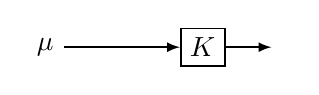
\begin{tikzpicture}[-latex ,auto ,node distance =2 cm and 3cm ,on grid ,
semithick ,
variable/.style ={ circle ,top color =white , 
draw , text=blue , minimum width =1 cm},
kernel/.style={rectangle,draw}
]
\node[kernel] (K) [left] {$K$};
\node (A) [left of = K] {$\mu$};
\node (E) [right = 1cm of K] {};
\draw (A) -- (K);
\draw (K) -- (E);
\end{tikzpicture}
\end{center}

represents the measure
\begin{align}
    \pi (A\times B)=\int_A \mu(dx_1) \int_B K(x_1, dx_2),\qquad A\in \mathcal{E}, B\in\mathcal{F}
\end{align}

This can be applied recursively, so given kernels $K_1$ from $(E,\mathcal{E})$ to $(F,\mathcal{F})$ and $K_2$ from $(F,\mathcal{F})$ to $(G,\mathcal{G})$, the diagram

\begin{center}
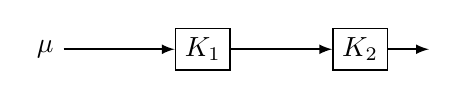
\begin{tikzpicture}[-latex ,auto ,node distance =2 cm and 3cm ,on grid ,
semithick ,
variable/.style ={ circle ,top color =white , 
draw , text=blue , minimum width =1 cm},
kernel/.style={rectangle,draw}
]
\node[kernel] (K1) [left] {$K_1$};
\node[kernel] (K2) [right of = K1] {$K_2$};
\node (A) [left of = K1] {$\mu$};
\node (E) [right = 1cm of K2] {};
\draw (A) -- (K1);
\draw (K1) -- (K2);
\draw (K2) -- (E);
\end{tikzpicture}
\end{center}

represents the measure
\begin{align}
    \pi (A\times B\times C)=\int_A \mu(dx_1) \int_B K_1(x_1, dx_2) \int_C K_2(x_2,dx_3),\qquad A\in \mathcal{E}, B\in\mathcal{F}, C\in \mathcal{G}
\end{align}

It is also possible to apply kernels ``in parallel''. Given kernels $K_a$ from $(E,\mathcal{E})$ to $(F,\mathcal{F})$ and $K_b$ from $(E,\mathcal{E})$ to $(G,\mathcal{G})$, the diagram

\begin{center}
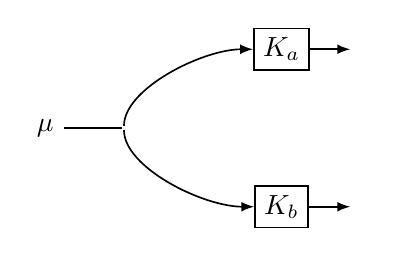
\begin{tikzpicture}[-latex ,auto ,node distance =1 cm and 4cm ,on grid ,
semithick ,
variable/.style ={ circle ,top color =white , 
draw , text=blue , minimum width =1 cm},
kernel/.style={rectangle,draw}
]
\node (A) [left] {$\mu$};
\node[inner sep=0pt] (S) [right = 1cm of A] {};
\node[kernel] (Ka) [above right = 1cm and 2cm of S] {$K_a$};
\node[kernel] (Kb) [below right = 1cm and 2cm of S] {$K_b$};
\node (E) [right = 1cm of Ka] {};
\node (F) [right = 1cm of Kb] {};
\draw[-] (A) -- (S);
\draw (S) .. controls +(down:5mm) and +(left:10mm) .. (Kb);
\draw (S) .. controls +(up:5mm) and +(left:10mm) .. (Ka);
\draw (Ka) -- (E);
\draw (Kb) -- (F);
\end{tikzpicture}
\end{center}

represents the measure
\begin{align}
    \pi (A\times B\times C)=\int_A \mu(dx_1) \int_B K_a(x_1, dx_2) \int_C K_b(x_1,dx_3),\qquad A\in \mathcal{E}, B\in\mathcal{F}, C\in \mathcal{G}
\end{align}

Parallel and series application can be interchangeably composed. These diagrams are based on the work of Fong \cite{fong_causal_2013}.

\end{definition}

We define measure spaces for the history $H$, observations $A$, outcomes $V$, interventions $I$ and policy index $Q$ in Table \ref{tab:measure_spaces}.
We further define Markov kernels for observation $\theta$, policy choice $\pi$, policy implementation $\phi$ and resolution $\mu$. The history $H$ is equipped with a probability measure $P_H$.

% \begin{table}[h]
%     \centering
%     \begin{tabular}{c|c|c|c}
%         Name & Set & $\sigma$-algebra & Probability Measure \\
%         \hline
%         History & $H$ & $\mathcal{H}$ & $P_H$ \\
%         Observations & $A$ & $\mathcal{A}$ & $P_H \theta$\\
%         Outcomes & $V$ & $\mathcal{V}$ & $P_H^3 \mu (\mathbb{I}\times \phi) (\mathbb{I}\times \theta \times \pi)$\\
%         Interventions & $I$ & $\mathcal{I}$ & $P_H^2 \phi (\theta_t \times \pi_t)$ \\
%         Policy index & $Q$ & $\mathcal{Q}$ & $P_H \pi$
%     \end{tabular}
%     \caption{Measure space names and definitions}
%     \label{tab:measure_spaces}
% \end{table}
\begin{table}[h]
    \centering
    \begin{tabular}{c|c|c|c}
        Name & Set & $\sigma$-algebra & Intuition \\
        \hline
        History & $H$ & $\mathcal{H}$ & Everything that could have a causal effect on $I$ or $V$ \\
        Accounted Variables & $A$ & $\mathcal{A}$ & Variables that are accounted for in the choice of intervention\\
        Outcomes & $V$ & $\mathcal{V}$ & Variables that are relevant to the cost \\
        Interventions & $I$ & $\mathcal{I}$ & Things that we're permitted to ``do''  \\
        Unaccounted Variables & $Q$ & $\mathcal{Q}$ & Variables that affect the choice of intervention but are unaccounted for
    \end{tabular}
    \caption{Measure space names and definitions}
    \label{tab:measure_spaces}
\end{table}

\begin{table}[h]
    \centering
    \begin{tabular}{c|c|c}
        Name & Symbol & Type signature  \\
        \hline
        Observation & $\theta$ & $H\to \Delta(\mathcal{A})$ \\
        Policy choice & $\pi$ & $H\to \Delta(\mathcal{Q })$ \\
        Policy implementation & $\phi$ & $A\times Q\to \Delta(\mathcal{I})$ \\
        Resolution & $\mu$ & $H\times I \to \Delta(\mathcal{V})$  \\
    \end{tabular}
    \caption{Markov kernel definitions.}
    \label{tab:kernels}
\end{table}

\begin{table}[h]
    \centering
    \begin{tabular}{c|c|c}
        Symbol & Type signature & Function  \\
        \hline
        & & \\
        $\hat{S}$ (for any measurable set $S$) & $S\to S$ & Identity: $\hat{S}(s)=s$ \\
    \end{tabular}
    \caption{Random variable definitions.}
    \label{tab:kernels}
\end{table}

Consider the joint probability measure $P:\mathcal{H}\times \mathcal{A}\times \mathcal{I}\times \mathcal{Q}\times \mathcal{V}\to [0,1]$ defined by the following composition of $P_H$ and kernels in table \ref{tab:kernels}:

\begin{center}
\begin{tikzpicture}[-latex ,auto ,node distance =1 cm and 4cm ,on grid ,
semithick ,
variable/.style ={ circle ,top color =white , 
draw , text=blue , minimum width =1 cm},
kernel/.style={rectangle,draw}
]
\node[kernel] (Kmu) [right] {$\mu$};
\node[kernel] (Kphi) [above left = 2cm and 2cm of Kmu] {$\phi$}
    edge[bend left] (Kmu);
\node[kernel] (Ktheta) [above left = 1cm and 2cm of Kphi] {$\theta$}
    edge[bend left] (Kphi);
\node[kernel] (Kpi) [below left = 1cm and 2cm of Kphi] {$\pi$}
    edge[bend right] (Kphi);
\node[inner sep=0pt] (S) [below left = 1cm and 2cm of Ktheta] {}
    edge[bend left] (Ktheta)
    edge[bend right] (Kpi)
    edge[bend right = 50] (Kmu);
\node (A) [left = 1cm of S] {$P_H$}
    edge[-] (S);
\draw (Kmu.east) -- +(1,0);
\end{tikzpicture}
\end{center}

If we take the sets $H,A,V,I,Q$ to be countable with discrete $\sigma$-algebras, the probability distribution generated by this composition can be written

\begin{align}
    P(h,a,q,i,v) = P_H(h)\theta(h,a)\pi(h,q)\phi(q,a,i)\mu(h,i,v)
\end{align}

We will call the distribution $P$ the causal model generated by $P_H(h)$ and the kernels $\theta,\pi,\phi,\mu$.

Using a more familiar graphical notation, this probability distribution factorises according to the following DAG, which can make it easy to work out conditional independences:

\begin{center}
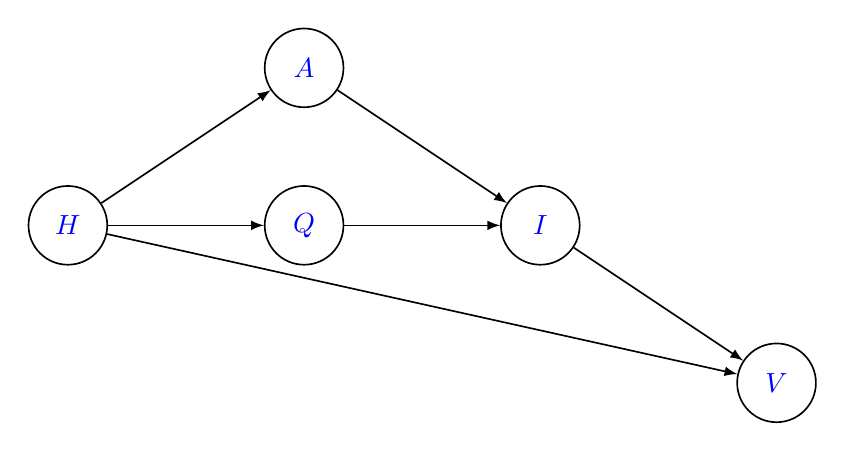
\begin{tikzpicture}[-latex ,auto ,node distance =2 cm and 3cm ,on grid ,
semithick ,
state/.style ={ circle ,top color =white ,
draw , text=blue , minimum width =1 cm}]
\node[state] (H) [left] {$H$};
\node[state] (A) [above right = of H] {$A$};
\node[state] (Q) [right = of H] {$Q$};
\node[state] (I) [right = of Q] {$I$};
\node[state] (V) [below right = of I] {$V$};
\draw (H) -- (A);
\draw (H) -- (Q);
\draw (H) -- (V);
\draw (A) -- (I);
\draw (Q) -- (I);
\draw (I) -- (V);
\end{tikzpicture}
\end{center}

Some notes on this setup:
\begin{itemize}
    \item $P$ is a very model in which an intervention $I$ and an outcome $V$ are resolved by arbitrary Markov kernels from some history $H$ and (need to prove arbitrary kernel $K:H\to I$ can be "factored" in to $\pi$, $\theta$ and $\phi$)
    \item A model formed by composition of Markov kernels is quite similar to an instance of a structural causal model (definition \ref{def:structural_equation})
    \item Any fixed value of $Q$ corresponds to a particular Markov kernel $\phi(\cdot,q,\cdot):A\to \Delta (\mathcal{I})$
\end{itemize}

\subsection{Policy-based causal identifiability}

We are ultimately concerned with situations where an agent wants to minimise a cost $C:\Delta (I\times V)\to \mathbb{R}$. If we suppose the agent knows the joint probability $P(i,a,v) = \sum_{q\in Q} P(q) P(v|i,a,q) \phi(a,q,i) P(a|q) $, a simple approach to minimising the cost would be to choose a kernel $\phi_{q^*}\in \Phi_u$ where $\Phi_q=\{\phi(\cdot,q,\cdot)|q\in Q\}$ is a set of kernels $A\to\Delta(\mathcal{I})$ and

\begin{align}
    \phi_{\tilde{q}}(a,i) = \argmin_{\phi_q\in \Phi_q} C \left( \sum_A P(V|I,A) \phi_q(A,I) P(A)\right)
\end{align}

By construction, there exists $\tilde{q}\in Q$ such that $\phi_{\tilde{q}}=\phi(\cdot,\tilde{q},\cdot)$. It may not be the case, however, that $\tilde{q}$ is in fact the policy that optimises the cost.

\begin{example}[Useless medicine]
We use the example of useless medicine to illustrate where naive cost minimization might go awry. $S:\mathcal{H}\to \{0,1\}$ is information on whether or not someone is sick, $I=\{0,1\}$ is a variable representing whether or not they received treatment and $V=\{0,1\}$ is a variable representing whether or not they recovered. We are aiming (perhaps unwisely) to maximise recovery, while avoiding unnecessary treatment: $C(P(i,v))=-\mathbb{E}[V-0.5I]$. 

Suppose that the treatment does nothing, but sick people always recover anyway: $P(v|i,s) = P(v|s) = \delta_{vs}$. Suppose furthermore that only sick people are treated. That is, given $Q=\{0,1\}$ and $\phi$ such that $\phi(\_,q,i)=\delta_{qi}$, we have $\pi(q,s)=\delta_{qs}$. We take $A=\emptyset$

The above assumptions lead straightforwardly to $P(v|i)=\delta_{vi}$, a typical case of ``correlation is not causation''. Recovery is perfectly matched with treatment, but this is contingent on the unwise choice of policy in which only sick people were treated. If people were treated randomly we would find that recovery was independent of treatment.

Returning to our cost function, it would naively appear that the policy $\phi_{q1}:A\mapsto \delta_{i1}$ is optimal:

\begin{align}
    C(P(v|i)\delta_{i1}) &= 0.5\\
    C(P(v|i)\delta_{i0}) &= 0
\end{align}

However, if we adjust for $S$ we find that we should not treat. $P(v|i,q,s)=P(v|s)$ and so $P(i,v|q,s)=P(v|s)P(i|q)$ and

\begin{align}
    C(P(v|s)P(i|q)) = 0.5q - s
\end{align}

Here, the problem was that the set $A=\emptyset$ was not large enough. If $S$ were in $\mathcal{A}$ we could have correctly concluded that sickness and not treatment was driving recovery.
\end{example}

We are interested in conditions under which some procedure will allow an agent to find an optimal policy  $\phi_*: A\to \Delta(\mathcal{I})$. There are two competing notions for optimality, which are loosely associated with the competing schools of Causal Decision Theory (CDT) and Evidential Decision Theory (EDT).

We index notions of optimality with elements $\mathbf{h}_\alpha$ of sub-$\sigma$-algebras of $\mathcal{H}$. This is because in general the conditions under which we optimize may be different from the conditions under which we collect data (e.g. "test" vs "deployment" or "experimental" vs "real-world" environments), which we will label $\mathbf{h}_0$ and $\mathbf{h}_\alpha$ respectively. In particular, the marginal probabilities $P(q|\mathbf{h}_0)\neq P(q|\mathbf{h}_\alpha)$.

\begin{definition}[$\mathbf{h}_\alpha$-counterfactual optimality]
Given a causal model $P$ generated by $\langle P_H,\theta,\pi,\phi,\mu\rangle$ and $\pi':H\to \Delta(Q)$, define $P_{\pi'}$ as the model generated by $\langle P_H,\theta,\pi,\phi,\mu\rangle$. For each $q\in Q$, define $\pi_q:H\mapsto \delta_q$. Given a sub-$\sigma$-algabra $\mathcal{H}_\alpha$ of $\mathcal{H}$, the $\mathbf{h}_\alpha$-counterfactually optimal policy choice is
\begin{align}
    q^*_{cf}=\argmin_{q\in Q}C(P_{\pi_q}(i,v|\mathcal{H}_\alpha=\mathbf{h}_\alpha))
\end{align}
\end{definition}

\begin{remark}
$P_{\pi_q}(\cdot)$ could also be written as $P(\cdot|do(Q=q))$.
\end{remark}

\begin{definition}[$\mathbf{h}_\alpha$-conditional optimality]
Given a causal model $P$ generated by $\langle P_H,\theta,\pi,\phi,\mu\rangle$ and a sub-$\sigma$-algabra $\mathcal{H}_\alpha$ of $\mathcal{H}$ and $\mathbf{h}_\alpha \in \mathcal{H}_\alpha$, the $\mathbf{h}_\alpha$-conditionally optimal policy choice is
\begin{align}
    q^*_{cd} = \argmin_{q\in Q} C(P(i,v|q,\mathcal{H}_\alpha=\mathbf{h}_\alpha))
\end{align}
\end{definition}

\begin{definition}[Agnostic optimality]
A policy choice $q^*$ is $\mathbf{h}_\alpha$-agnostically optimal if $q^*=q^*_{cd}=q^*_{cf}$.
\end{definition}

\begin{definition}[$\mathbf{h}_0,\mathbf{h}_\alpha$-Optimizability]
A causal model $P$ along with sub-$\sigma$-algebras $\mathcal{H}_0,\mathcal{H}_\alpha\subset \mathcal{H}$ is $\mathbf{h}_0,\mathbf{h}_\alpha$-optimizable if, given  $P(i,a,v|\mathcal{H}_0=\mathbf{h}_0)$, it is possible to find a $\mathbf{h}_\alpha$-optimal $q\in Q$.

Here ``optimal'' is understood to be any of counterfactually optimal, conditionally optimal or agnostically optmial.
\end{definition}

\textbf{Note: } $P(i,a,v|\mathcal{H}_\cdot=h_\cdot)=\mathbb{E}[\mathds{1}_{I=i,A=a,V=v}|\mathcal{H}_\cdot=h_\cdot]$

Noting that the naive approach to optimising the cost may not be the only possibility, we will for now ask under what conditions it does yield an optimal policy selection. We will assume that the joint probability $P(i,a,v|\mathcal{H}_0=\mathbf{h}_0)$ is known, and the proposed policy choice is

\begin{align}
    \tilde{q} = \argmin_{q\in Q} C \left( \sum_{a\in A} P(v|i,a,\mathbf{h}_0) \phi(a,q,i) P(a|\mathbf{h}_0)\right)
\end{align}

Note that this strategy ought to work if the quantity $\sum_a P(v|i,a) \phi_q(a,i) P(a) = P(i,v|q)$ for all $q\in Q$. We will formalise this below:

\begin{definition}[$\mathbf{h}_0$-Identifiability]
A model $P$ along with $\mathcal{H}_0\subset\mathcal{H}$ is $\mathbf{h}_0$-identifiable if for all $q,q'\in Q$
\begin{align}
    \sum_{a\in A} P(i,a,v|q,h_\beta)=\sum_{a\in A} P(v|i,a,q',h_\beta) \phi(a,q,i) P(a|q',h_\beta) 
\end{align}
Where $P(\cdot | \mathbf{h}_0)=P(\cdot | \mathcal{H}_0 = \mathbf{h}_0)$
\end{definition}

\begin{definition}[$\mathbf{h}_0$-Policy exchangeability]
A model $P$ along with $\mathcal{H}_0\subset\mathcal{H}$ is $\mathbf{h}_0$-policy exchangeable if for all $q,q'\in Q$
\begin{align}
    P(v|i,a,q,\mathbf{h}_0) = P(v|i,a,q',\mathbf{h}_0)
\end{align}
Where $P_{\mathbf{h}_0}=P(h,q,a,i,v|\mathcal{H}_\beta=\mathbf{h}_0)$. If $\phi(a,q,i)=0$, then $P(v|i,a,q,\mathbf{h}_0)$ may be defined by substituting $\phi_{\epsilon}(a,q,i) = (1-\epsilon)\phi(a,q,i) + \epsilon$ for $\phi$ and taking the limit of $\phi_{\epsilon}$ as $\epsilon \to 0$.
\end{definition}

\begin{definition}[$\mathbf{h}_0$-Policy uncorrelatedness]
A model $P$ along with $\mathcal{H}_0\subset\mathcal{H}$ is $\mathbf{h}_0$-policy uncorrelated if for all $q\in Q$

\begin{align}
    \sum_{a\in A} P(v|i,a,q,\mathbf{h}_0)\phi(a,q,i) P(a|q,\mathbf{h}_0) = \sum_{a\in A} P(v|i,a,q,\mathbf{h}_0)\phi(a,q,i) P(a|\mathbf{h}_0)
\end{align}

A particularly simple case of policy uncorrelatedness is when
\begin{align}
    A\CI_{P_{\mathbf{h}_0}} Q
\end{align}
\end{definition}

\begin{definition}[$\mathbf{h}_0,\mathbf{h}_\alpha$-stability]
Given sub-$\sigma$-algebras $\mathcal{H}_0,\mathcal{H}_\alpha\subset \mathcal{H}$, a model $P$ is $\mathbf{h}_0,\mathbf{h}_\alpha$-outcome-stable if
\begin{align}
    P(v|i,a,q,\mathbf{h}_0) = P(v|i,a,q,\mathbf{h}_\alpha)
\end{align}

A model $P$ is $\mathbf{h}_0,\mathbf{h}_\alpha$-observation-stable if
\begin{align}
    P(a|q,\mathbf{h}_0) = P(a|q,\mathbf{h}_\alpha)
\end{align}

A model $P$ is $h0,\mathbf{h}_\alpha$-stable iff it is $\mathbf{h}_0,\mathbf{h}_\alpha$-outcome-stable and $\mathbf{h}_0,\mathbf{h}_\alpha$-observation-stable.

\end{definition}

\begin{definition}[Common support]
% A model $P$ has $h_\beta$-common policy support if for all $h\in h_\beta$, $q\in Q$
% \begin{align}
%     \pi(h,q) > 0
% \end{align}
A model $P$ has $h_\beta$-common observation support if for all $a\in A$, $q\in Q$
\begin{align}
    P(a|q) > 0
\end{align}

A model $P$ has $h_\beta,q$-common intervention support if for all $i\in I$, $a\in A$
\begin{align}
    \phi(a,q,i) > 0
\end{align}

A model with common observation and common intervention support has common support.
\end{definition}

\begin{theorem}[Policy Exchangeability and Uncorrelatedness implies Identifiability]
A model $P_H(h),\theta,\pi,\phi,\mu$ that is $h_\beta$-policy exchangeable and $h_\beta$-policy uncorrelated is $h_\beta$-identifiable.
\end{theorem}

\begin{proof}
For any $q\in Q$
\begin{align}
    \sum_{a\in A} P_{h_\beta}(v,i,a|q) &= \sum_{a\in A} P_{h_\beta}(v|i,a,q)\phi(a,q,i) P_{h_\beta}(a|q) \\
                             &= \sum_{a\in A} P_{h_\beta}(v|i,a,q) \phi(a,q,i) P_{h_\beta}(a|q')\qquad\forall q'\in Q\text{ (policy uncorrelatedness)}\\
                             &= \sum_{a\in A} P_{h_\beta}(v|i,a,q') \phi(a,q,i) P_{h_\beta}(a|q')\qquad\text{(policy exchangeability)}
\end{align}
\end{proof}

\begin{theorem}[$\mathbf{h}_0$-identifiability + $\mathbf{h}_0$ common support + $\mathbf{h}_\alpha,\mathbf{h}_0$-stability implies $\mathbf{h}_\alpha,\mathbf{h}_0$-conditional optimizability]\label{th:conditional_optzy}
Given a model $P$, it is possible to find an $\mathbf{h}_\alpha$-conditionally optimal $q^*_{cd}$ given $P(a,i,v|\mathbf{h}_0)$ if $P$ is $\mathbf{h}_0$-identifiable and $\mathbf{h}_\alpha,\mathbf{h}_0$-stable.
\end{theorem}

\begin{proof}
We have for all $q\in Q$

\begin{align}
   P(i,v|q,\mathbf{h}_\alpha)&=\sum_{a\in A} P(v|i,a,q,\mathbf{h}_0) \phi(a,q,i) P(a|q,\mathbf{h}_0) \qquad\text{(stability)}\\
                    &=\sum_{a\in A} P(v|i,a,\mathbf{h}_0) \phi(a,q,i) P(a|\mathbf{h}_0) \qquad (\mathbf{h}_0\text{-identifiability})\\
                    &=\sum_{a\in A} \frac{P(a,i,v|\mathbf{h}_0)}{P(a,i|\mathbf{h}_0)} \phi(a,q,i) P(a|\mathbf{h}_0)\qquad\text{(common support)}
\end{align}

for conditional $\mathbf{h}_0,\mathbf{h}_\alpha$-optimizability:
\begin{align}
    q^*_{cd} &= \argmin_{q\in Q} P(i,v|q,\mathbf{h}_\alpha)
\end{align}
\end{proof}

Counterfactual optimizability follows from an alternative, stronger version of the exchangeability assumption. On the other hand, we drop the stability assumption as it is something we will revisit later.

\begin{definition}[$\mathbf{h}_0$-Counterfactual policy exchangeability]
A model $P$ along with $\mathcal{H}_0\subset\mathcal{H}$ is $\mathbf{h}_0$-counterfactually policy exchangeable if for all $q\in Q$ and all kernels $\pi_q:h\mapsto \delta_q$:
\begin{align}
    P(v|i,a,q,\mathbf{h}_0) = P_q(v|i,a,\mathbf{h}_0)
\end{align}
Where $P_q$ is the causal model generated by replacing $\pi$ with $\pi_q$ in the set of kernels generating $P$.
\end{definition}

\begin{lemma}[Counterfactual exchangeability implies exchangeability]\label{le:cfex_im_ex}
If a model $P$ is $\mathbf{h}_0$-counterfactually exchangeable then it is $h0$-exchangeable.
\end{lemma}

\begin{proof}
For all $q,q'\in Q$
\begin{align}
    P_q(v|i,a,\mathbf{h}_0) &= \frac{\sum_{h\in \mathbf{h}_0, x\in Q} \mu(i,h,v) \phi(a,q,i) \theta(h,a)\delta_{xq} P_H(h|\mathbf{h}_0)}{\sum_{h\in \mathbf{h}_0, x\in Q} \phi(a,q,i)\theta(h,a)\delta_{xq} P_h(h|\mathbf{h}_0)}\\
                    &= \frac{\sum_{h\in \mathbf{h}_0}\mu(i,h,v)\theta(h,a)P_H(h|\mathbf{h}_0)}{\sum_{h\in \mathbf{h}_0} \theta(h,a) P_H(h|\mathbf{h}_0)}\\
                    &= P_{q'}(v|i,a,\mathbf{h}_0)
\end{align}

Then we have for all $q,q'\in Q$
\begin{align}
    P(v|i,a,q,\mathbf{h}_0) &= P_q(v|i,a,\mathbf{h}_0) \\
                   &= P_q'(v|i,a,\mathbf{h}_0) \\
                   &= P(v|i,a,q,\mathbf{h}_0)
\end{align}
\end{proof}

\begin{corrolary}[Counterfactual exchangeability and policy exchange]\label{corr:cfex_pex}
If follows from Lemma \ref{le:cfex_im_ex} that if a model $P$ is $\mathbf{h}_0$-counterfactually exchangeable then for all $q,q'\in Q$
\begin{align}
    P(v|i,a,\mathbf{h}_0) = P_{q'}(i,a,\mathbf{h}_0)
\end{align}
\end{corrolary}



\begin{theorem}[$\mathbf{h}_0$-counterfactual exchangeability + $\mathbf{h}_0$-policy uncorrelatedness + $\mathbf{h}_0$-common support +  implies $\mathbf{h}_0$-counterfactual optimizability]

Given a model $P$, it is possible to find an $\mathbf{h}_0$-counterfactually optimal $q^*_{cf}$ given $P(a,i,v|\mathbf{h}_0)$ if $P$ is $\mathbf{h}_0$-counterfactually exchangeable, $\mathbf{h}_0$-policy uncorrelated and has $\mathbf{h}_0$-common support.
\end{theorem}

\begin{proof}

From Corollary \ref{corr:cfex_pex}, we have for all $q\in Q$
\begin{align}
    P(v|i,a,\mathbf{h}_0) = P_{q}(v|i,a,\mathbf{h}_0) \label{eq:cfex}
\end{align}

We also have for any $q\in Q$
\begin{align}
    P_q(a|\mathbf{h}_0) &= \sum_{h\in \mathbf{h}_0} \theta(h,a) P_H(h|\mathbf{h}_0) \nonumber\\
               &= P(a|\mathbf{h}_0)\qquad \text{(Policy uncorrelatedness)} \label{eq:cfun}
\end{align}

Thus, for any $q\in Q$
\begin{align}
    P_q(i,v|\mathbf{h}_0) &= \sum_{a\in A} P_q(v|i,a,\mathbf{h}_0) \phi(a,q,i) P_q(a|\mathbf{h}_0) \\
                 &= \sum_{a\in A} P(v|i,a,\mathbf{h}_0) \phi(a,q,i) P(a|\mathbf{h}_0) \\
                 &= \sum_{a\in A} \frac{P(a,i,v|\mathbf{h}_0)}{P(a,i|\mathbf{h}_0)} \phi(a,q,i) P(a|\mathbf{h}_0) \qquad\text{(common support)}
\end{align}

It is then straightforward to find
\begin{align}
    q^*_{cf} = \argmin_{q\in Q} (P_q(i,v|\mathbf{h}_0))
\end{align}
\end{proof}

\subsection{Relating the conditional and counterfactual perspectives}

The relationship between the conditional and counterfactual perspectives and the identifiability assumptions are significantly simplified by introducing sun-$\sigma$-algebras associated with the kernels $\mu$, $\pi$ and $\theta$:

\begin{align}
    \mathcal{H}_\mu &= \sigma(\cup_{\mathbf{v}\in \mathcal{V}} \mu^{-1}(\mathcal{H},\mathbf{v}))\\
    \mathcal{H}_\pi &= \sigma(\cup_{\mathbf{q}\in \mathcal{Q}} \mu^{-1}(\mathcal{H},\mathbf{q}))\\
    \mathcal{H}_\theta &= \sigma(\cup_{\mathbf{a}\in \mathcal{A}} \mu^{-1}(\mathcal{H},\mathbf{a}))\\
\end{align}

where for some kernel $K$ from $(E,\mathcal{E})$ to $(F,\mathcal{F})$ and $B\in \mathcal{F}$:
\begin{align}
    K^{-1}(\mathcal{E},B) &= \{K^{-1}(A,B)|A\in\sigma([0,1])\} \\
    K^{-1}(A,B) &= \{e|K(e,B)\in A\}
\end{align}

For each $q\in Q$, define $\tilde{\mathbf{h}}_q=\{\mathbf{h}|\mathbf{h}\in \mathcal{H}\wedge \phi(h,q')=\delta_{qq'}\forall h\in \mathbf{h}\}$ and consider the set $\mathbf{h}_q=\cap_{\mathbf{h}\in \tilde{\mathbf{h}}_q}\mathbf{h}$. For any non-empty $\mathbf{h}_q$, we have $P(h,q,a,i,v|\mathbf{h}_q)=P_q(h,q,a,i,v|\mathbf{h}_q)$. 

Then, for any model that is $\mathbf{h}_0,\mathbf{h}_q$-stable, we have
\begin{align}
    P(v|i,a,q,\bf{h}_0) = P_q(v|i,a,\bf{h}_q)
\end{align}


% In either case, we have for $q\in Q$
% \begin{align}
%     P(I_0,V_0|q) &= \int_{A} P(da|q) \int_{I_0} P(di|a,q) \int_{V_0} P(dv|i,a,q) \\
%                  &= \int_{A} P(da|q) \int_{I_0} \phi(a,q,di) \int_{V_0} P(dv|i,a,q)
% \end{align}

Additionally, we need to ensure that we can estimate $P(v|i,a)$ and $P(a)$. That is, we require \emph{common support}:
\begin{align}
    \phi(a,q,i) &> 0  \qquad \text{for all }a\in A, i\in I \\
    P(a|q) &> 0 \qquad \text{for all }a\in A
\end{align}

The setting so far is quite abstract, and it's not necessarily obvious when we should expect Equations \ref{eq:policy_choice} and \ref{eq:policy_exchange} to hold. An intuitively appealing situation in which these assumptions \emph{do} hold is where $V$ and $Q$ each depend on independent components of $H$.

Suppose we introduce Markov kernels $\nu_A:H\to\Delta(H_A)$ and $\nu_Q:H\to\Delta(H_Q)$ and redefining $\pi$, $\theta$ and $\mu$ such that $\theta:H_A\to \Delta(A)$, $\pi:H_Q\to \Delta(Q)$ and $\mu:H_A\times I\to \Delta (V)$. Again abusing notation to let set names also stand for random variables given by identity functions, suppose that we have $H_A \CI H_Q$.

These properties allow us to draw a modified Bayesian network for $P$, substituting $H_A$ and $H_Q$ for $H$. Via the d-separation criterion, we clearly have conditions \ref{eq:policy_choice} and \ref{eq:policy_exchange}.
\textbf{Prove this}

\begin{center}
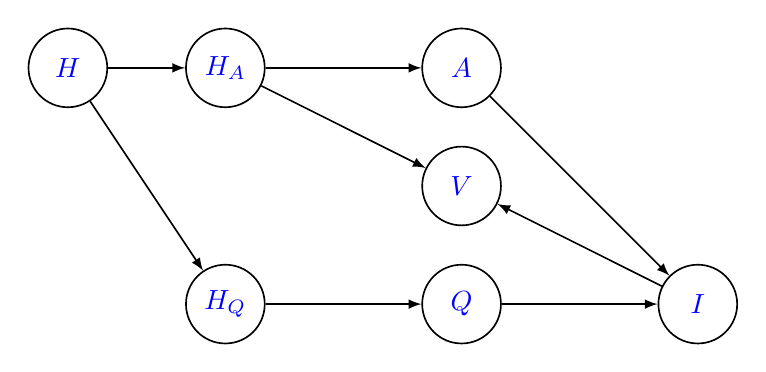
\begin{tikzpicture}[-latex ,auto ,node distance =2 cm and 3cm ,on grid ,
semithick ,
state/.style ={ circle ,top color =white ,
draw , text=blue , minimum width =1 cm}]
\node[state] (H) [left] {$H$};
\node[state] (H_A) [right of = H] {$H_A$};
\node[state] (H_Q) [below = 3cm of H_A] {$H_Q$};
\node[state] (A) [right = of H_A] {$A$};
\node[state] (Q) [right = of H_Q] {$Q$};
\node[state] (I) [right = of Q] {$I$};
\node[state] (V) [below right = 1.5cm and 3cm of H_A] {$V$};
\draw (H) -- (H_A);
\draw (H) -- (H_Q);
\draw (H_A) -- (A);
\draw (H_Q) -- (Q);
\draw (H_A) -- (V);
\draw (A) -- (I);
\draw (Q) -- (I);
\draw (I) -- (V);
\end{tikzpicture}
\end{center}

Given the assumed independence of $H_A$ and $H_Q$, the independences \ref{eq:policy_choice} and \ref{eq:policy_exchange} follow from these assumptions.

\textbf{Proof sketch: } \emph{Conjecture} Because $H_A$ is independent of $H_Q$ and all dependence on $H$ is screened off by these variables, independence relations among the rest of the variables can be found by d-separation on the graph formed by deleting $H$.

Independences \ref{eq:policy_choice} and \ref{eq:policy_exchange} follow from d-separation on this modified graph. $\square$

This stronger set of assumptions, I think, maps reasonably well to ordinary intuitions about why we should expect an idealised randomised trial to give us policy relevant information. We expect that the choice of treatment assignment function $Q$ is influenced by factors that are independent of anything that influences the outcomes $V$. If the treatment assignment $I$ does depend on any outcome-related variables $H_A$, this influence is screened off by the observed set $A$, which we know because we have dictated the relationship between $A$ and $I$. Finally, the map $\phi(\cdot,q,\cdot)$ from $A$ to $I$ must be sufficiently random in order to achieve common support. 

\subsubsection{Connection to CBN identifiability}

Commonalities:

\begin{itemize}
    \item There's a natural identification of $P(V|do(I=i_0))$ with a policy choice $q_0$ such that $\phi(a,q_0,\{i\}):A\mapsto \delta_{ii_0}$ for all $a\in A$.
    \item The argument above considers probability spaces related by Markov kernels, which generate Bayesian networks. As such, independence results for Bayesian networks are relevant
    \item In particular, the ``independent histories'' assumption produces a graph in which the backdoor criterion does hold for the effect of $I$ on $V$
\end{itemize}

Differences:

\begin{itemize}
    \item The policy based approach works with regular Bayesian networks without $do()$ operations. I believe there are variables that can be represented this way that can't be represented in a Bayesian network with a $do()$ operation (e.g. two-way interactions), but I need to show this
    \item I believe that if we adopt a time dependent approach (i.e. introduce sub-$\sigma$-algebras $\mathcal{H}_t\subset \mathcal{H}$ that capture the set of possible histories up to $t$), there are cases where knowing $P(V|do(I=i))$ for each $i\in I$ is insufficient to deduce the optimal policy $Q$. Again, I need to show this.
\end{itemize}

\subsubsection{Connection to potential outcomes identifiability}

Commonalities:

\begin{itemize}
    \item There's a natural identification of the potential outcomes idea of a true outcome $V(1)$ with a policy choice $q_1$ such that $\phi(a,q_1,\{i\}):A\mapsto \delta_{i1}$ for all $a\in A$.
    \item Under the identification above, the policy exchangeability assumption (\ref{eq:policy_exchange}) is a natural generalisation of the ignorability assumption
    \item The common support assumption is also present in the potential outcomes approach, though the common support assumption here includes the additional condition that $P(a|q) > 0$ for all $a\in A$
\end{itemize}

Differences:

\begin{itemize}
    \item Under a time dependent approach, ignorability may hold where policy exchangeability doesn't
    \item The potential outcomes approach doesn't involve composition of Markov kernels, and arguably doesn't formally distinguish between elements of $A$ which have a ``causal'' effect on intervention $I$ and elements of $V$ that are ``effects'' of $I$
    \item The potential outcomes approach doesn't feature a free policy choice assumption (\ref{eq:policy_choice}).
\end{itemize}


\subsection{Independence of Identifiability Assumptions}

Given that the potential outcomes approach features common support and policy exchangeability assumptions but not the free policy choice assumption, it is reasonable to ask whether these assumptions are independent. It turns out that they are.

\subsubsection{Policy Exchange and Policy Choice are independent}

Consider a randomised medical trial with variables $X,T\in \mathcal{A}$ where $X\in\{0,1\}$ is a variable indicating experimental conditions and $T$ is a variable summarising patient characteristics. Suppose that the joint distribution of variables is compatible with this graph:

\begin{center}
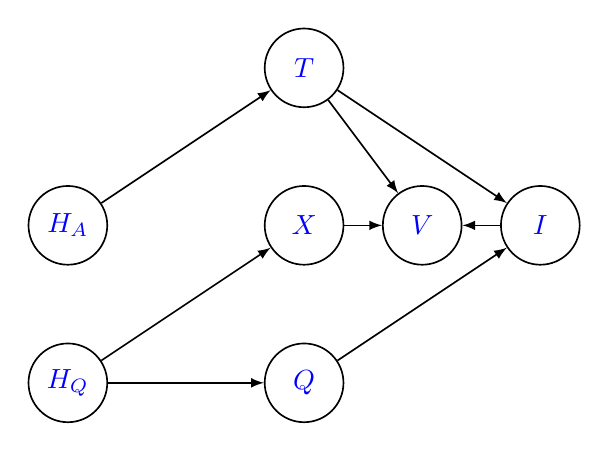
\begin{tikzpicture}[-latex ,auto ,node distance =2 cm and 3cm ,on grid ,
semithick ,
vble/.style ={ circle ,top color =white , 
draw , text=blue , minimum width =1 cm}
]
\node[vble] (Ha) [left] {$H_A$};
\node[vble] (Hq) [below of = Ha] {$H_Q$};
\node[vble] (Q) [right = 3cm of Hq] {$Q$}
    edge[latex-] (Hq);
\node[vble] (X) [right = 3cm of Ha] {$X$}
    edge[latex-] (Hq);
\node[vble] (T) [above of = X] {$T$}
    edge[latex-] (Ha);
\node[vble] (I) [right = 3cm of X] {$I$}
    edge[latex-] (T)
    edge[latex-] (Q);
\node[vble] (V) [right = 1.5cm of X] {$V$}
    edge[latex-] (X)
    edge[latex-] (T)
    edge[latex-] (I);
\end{tikzpicture}
\end{center}

In words, the outcome depends on the treatment, the patient characteristics and whether or not the treatment is administered under experimental conditions. Suppose also that $Q$ is such that under experimental conditions, $\phi$ is randomised over possible values of $I$, while under non-experimental conditions is is deterministic.

Note that $\{I,X\}$ d-separates $V$ from $Q$, so policy exchangeability holds. However, it is possible to postulate a treatment that is only effective under experimental conditions, in which case the policy suggested by measurements with randomised policy choice $Q$ will not be effective.

If we remove $X$ from the observed set $A$, $A$ will no longer d-separate $V$ from $Q$. However, $A$ is now d-separated from $Q$ by the empty set. Thus in this case policy choice holds, but policy exchangeability does not.

\subsubsection{Policy Exchange, Policy Choice and Common Support are independent}

In the example above, the common support assumption is violated - in particular, a randomised policy choice $Q$ always coincides with $X=1$. This is an extended common support assumption, however, not covered by the standard assumptions of the potential outcomes approach. Newcomb's problem is a more esoteric scenario in which the common support be made to hold, but policy exchange or policy choice can be made to fail independently.

Suppose an agent with observations $O$ implements a policy $\Phi$ from a set of $\epsilon$-deterministic policies $\Phi_\epsilon= \{\phi:O\to\Delta I|\phi(o,i)\in\{\epsilon,1-\epsilon\}\}$. Suppose there is additionally a variable $\overline{\Phi}$ in the agent's history such that $\Phi=\overline{\Phi}$. Thus, if we take $A=\{O,\overline{\Phi}\}$, we clearly don't have free policy choice: $P(A=(o,\phi)|\Phi=\phi)\neq P(A=(o,\phi)|\Phi=\phi')$ for $\phi'\neq \phi$.

There is also a predictor that observes $A$ and outputs prediction $q=\mathrm{argmax}_{q'}\overline{\Phi}(O,q')$. Note that by assumption, we have $P(Q=I)=1-\epsilon$. The outcome $V$ pays out deterministically at the following values for different choices of $Q$ and $I$:
\begin{table}[h]
    \centering
    \begin{tabular}{c|c|c}
            & Q=1 & Q=2  \\
            \hline
        I=1 & 1e6  & 0 \\
        I=2 & 1.1e6& 1e5
    \end{tabular}
    \caption{Newcomb's problem payoff $V$}
    \label{tab:newcombs_problem}
\end{table}

The agent's cost is $C=-\mathbb{E}[V]$

We have policy exchangeability, as $P(V|I,Q)=P(V|I,A)=P(V|I,A,\Phi)$. Furthermore, for every $\phi\in\Phi_\epsilon$ we have $\phi(a,i)\geq \epsilon$ for all $a\in A$, $i\in\{1,2\}$, so we have common support. This demonstrates the possibility of \ref{def:policy_exchange}$\wedge$\ref{def:common_support}$\wedge\neg$\ref{def:free_policy}.

Also consider the policies $\phi_1:\phi_1(o,1)=1-\epsilon$ and $\phi_2:\phi(o,2)=1-\epsilon$ for all $o\in O$. We then have
\begin{align}
    \mathbb{E}[V|\Phi=\phi_1] &= 1\mathrm{e}6 (1-\epsilon) + 1.1\mathrm{e}6 (\epsilon) \\
                              &= 1\mathrm{e}6 + \epsilon \mathrm{e} 5 \\
    \mathbb{E}[V|\Phi=\phi_2] &= (1-\epsilon)\mathrm{e}5
\end{align}

It is not hard to show that any $\phi$ with nonconstant dependency on $o$ is also worse than $\phi_1$, and that $\phi_1$ is therefore optimal.

Of note:
\begin{itemize}
    \item It is sometimes possible to find an optimal policy even if free policy choice is violated
    \item Standard causal theories don't explicitly assume free policy choice, so they're unable to relax it in this example and as a result suggest that $\phi_2$ is optimal
\end{itemize}


% Consider an agent with a set of variables $H$ comprising its history and a set of actions $I$ available. The agent has an observation function $\theta$ such that $A=\theta(H)$ and implements some policy $\psi:H \to \Delta I$ (not necessarily cost minimising). Denote the agent's policy choice by $\Psi$. 
% Suppose the agent wishes to minimise a cost defined over action $I$ and a set of future variables $V$, $C:\Delta(I\times V)\to \mathbb{R}$. Furthermore, suppose it does so using the following strategy (which may or may not be sound): observe $I$, $A$ and $V$ and for each $a\in A$ and $i\in I$ estimate $P(V|I=i,A=a,\Psi=\psi)$ and $P(A|\Psi=\psi)$. Then implement the policy given by the Markov kernel $\tilde{\phi}:A\times I \to [0,1]$ such that
% \begin{align*}
%     \tilde{\phi} = \text{argmin}_{\phi} C\left(\sum_{a\in A}P(V=v|I=i,A=a,\Psi=\psi)\phi(a,i) P_\psi(A=a|\Psi=\psi)\right)
% \end{align*}

% The question arises: when will this strategy successfully select a policy that is optimal in the sense that given observations $A$ there is no Markov kernel $\phi\in [0,1]^{A\times I}$ such that 
% \begin{align*}
%     &C\left(\sum_{a\in A}P(V=v|I=i,A=a,\Psi=\phi)\phi(a,i) P_\psi(A=a|\Psi=\phi)\right) < \\
%     &C\left(\sum_{a\in A}P(V=v|I=i,A=a,\Psi=\tilde{\phi})\tilde{\phi}(a,i) P_\psi(A=a|\Psi=\tilde{\phi})\right)
% \end{align*}
% ?

% For a simple example of where this approach won't work, suppose there is some unobserved $H_1\in H$ such that $H_1\sim\mathrm{Bernoulli}(0.5)$ and $V=H_1$, $C(P(I,V))=\mathbb{E}(I-2V)$ and $\psi(h,i)=\delta_{h_1 i}$. This is a classic case of ``correlation is not causation''; we have $V\not\CI_{P_\psi} I$ but $V\CI_{P_\psi} I | H_1$. The cost approach above will recommend the policy $\phi_1$ where $\phi_1(\cdot,i)=\delta_{i1}$. The actual costs are:
% \begin{align}
%     C\left(P_\psi(V=v|I=i)\delta_{i1}\right)&=-1\text{ but}\\
%     C\left(P_{\phi_1}(V=v|I=i)\delta_{i1}\right) &=-0.5 \\
%     C\left(P_{\phi_0}(V=v|I=i)\delta_{i1}\right) &=-1
% \end{align}

% \subsubsection{Assumptions for policy-based causal inference}

% % \begin{definition}[Causal Model]
% % Given a set of variables $\mathbf{X} = \{V,H,I\}$ and a set of Markov kernels $\Psi:\{H\to\Delta I\}$, a causal model is a map $P_{(\cdot)}: \Psi \to \Delta X$. We will write $P(\cdot|\Psi=\psi)=P_\psi(\cdot)\in \Delta X$.
% % \end{definition}

% % \begin{remark}
% % I'm not sure it's necessary to postulate a model of this type, but it substantially simplifies things.
% % \end{remark}

% \begin{definition}[Causal identification problem]\label{def:causal_ident_prob}
% A causal identification problem is a problem of  the form: Given sets of generating random variables $V,H,I$ and policy $\Psi$ where $P(I=i|H=h)=\Psi(h,i)$, sets of observed variables $V,A,I$ where $\theta(H)=A$ for some observation function $\theta$, and fixing $\Psi=\psi$, find $P(A,I,V|\Psi=\phi)$ for each $\phi\in [0,1]^{A\times I}$.
% \end{definition}

% The following four assumptions are sufficient for a causal identification problem to be solvable:
% \begin{definition}[Policy exchangeability]\label{def:policy_exchange}
% For all $\phi \in [0,1]^{A\times I}$ where $\phi(a,i)>0$,
% \[P(V|A=a,I=i,\Psi=\psi)=P(V|A=a,I=i,\Psi=\phi)\] 
% \end{definition}

% \begin{definition}[Free policy choice]\label{def:free_policy}
% For all $\phi\in [0,1]^{A\times I}$, $P(A|\phi)=P(A|\psi)$
% \end{definition}

% \begin{definition}[Common support]\label{def:common_support}
% For all $a\in A$ and $i\in I$ there exists $h\in O^{-1}(a)$ such that $\psi(a,i)>0$
% \end{definition}

% \begin{theorem}[Policy-based identifiability]
% Given a causal identification problem, if Assumptions \ref{def:policy_exchange}, \ref{def:free_policy} and \ref{def:common_support} hold, then $P(V=v|A=a,I=i,\Phi=\phi)=P(V=v|A=a,I=i,\Phi=\phi_{\mathrm{obs}})$ for all $(a,i):\phi(a,i)>0$ for all $\phi\in\Phi$. Such a problem is called \emph{identifiable}. 
% \end{theorem}

% \begin{proof}
% It is always possible to write
% \begin{align}
%     P(V=v,I=i|\Psi=\phi) &= \sum_{a\in A} \phi(a,i) P(V=v|I=i,A=a,\Psi=\phi) P(A=a|\Psi=\phi)
% \end{align}

% For any $\phi\in[0,1]^{A\times I}$,
% \begin{align}
%     P(V=v,I=i|\Psi=\phi)&=\sum_{a} P(V=v|A=a,I=i,\Psi=\phi)\phi(a,i)P(A=a|\Psi=\phi) \\
%             &= \sum_{a} P(V=v|A=a,I=i,\Psi=\psi)\phi(a,i)P(A=a|\Psi=\phi) \qquad \text{Assumptions \ref{def:policy_exchange} \& \ref{def:common_support}}\\
%             &= \sum_{a} P(V=v|A=a,I=i,\Psi=\psi)\phi(a,i)P(A=a|\Psi=\psi) \qquad \text{Assumption \ref{def:free_policy}}
% \end{align}

% \end{proof}

% \begin{remark}
% Assumptions \ref{def:policy_exchange} and \ref{def:free_policy} address counterfactual quantities, as $\Psi=\psi$ in all cases. There is a relationship between them, as a failure of exchangeability may be rectified by identifying additonal variables to include in $A$. However, if we make $A$ extremely large - for example, if we just let $A=H$, then we may find some dependence between $A$ and $\Psi$. I don't know if there's a neater way to capture this than what's been put down here.
% \end{remark}

% \begin{remark}
% The policy exchangeability assumption is similar to the potential outcomes assumption of ignorability, with two differences:
% \begin{itemize}
%     \item the set $A$ must be calculated from the history of the agent at the time that it computes $I$, which excludes the possibility that $A$ is an effect of $I$
%     \item the ignorability condition asserts exchangeability for a restricted set of policies: the observational policy $\psi$, and constant policies $\phi_j:(a,i)\mapsto \delta_{ij}$
% \end{itemize}
% \end{remark}

% \begin{remark}
% I am definitely not claiming these assumptions are necessary, only that they are sufficient.
% \end{remark}


% In an idealised randomised trial, we identify a domain $A$ and choose a policy $\psi:A\to \Delta I$. We assume that $A$ is not dependent on the particular choice of $\psi$ (but see below). We can argue that for exchangeability starting from a slightly weaker assumption:

% \begin{definition}[Weak exchangeability]
% For all $\phi\in [0,1]^{A\times I}$, $P(V|H=h,I=i,\Psi=\psi)=P(V|H=h,I=i,\Psi=\phi)$
% \end{definition}

% Note that given the domain of $\psi$ and any $\phi\in [0,1]^{A\times I}$ is $A$, we have 
% \begin{align}
%     \psi(h,i)&=\psi(h',i)\qquad \forall i\in I, h,h' \in H \\
%     P(I|H=h,\Psi=\psi) & = P(I|H=h',\Psi=\psi) \\
%     \implies P(H=h|I=i
% \end{align}

% % That is, $$

% % Then we have
% \begin{align}
%     P(V|A=a,I=i,\Psi=\psi)&=\sum_{h\in O^{-1}(a)} P(V|H=h,I=i,\Psi=\psi) P(H=h|I=i,\Psi=\psi) \\
%                           &=\sum_{h\in O^{-1}(a)} P(V|H=h,I=i,\Psi=\phi) P(H=h|I=i,\Psi=\psi) \qquad \text{Weak exchangeability}\\
%                           &=\sum_{h\in O^{-1}(a)} P(V|H=h,I=i,\Psi=\phi) P(H=h|I=i,\Psi=\phi) \qquad \text{Conditional independence of $H$ and $I$}\\
%                           &= P(V|A=a,I=i,\Psi=\phi)
% \end{align}

% \subsubsection{Assumptions \ref{def:policy_exchange}, \ref{def:free_policy} and \ref{def:common_support} are independent}

% \textbf{Assumptions \ref{def:policy_exchange} + \ref{def:common_support} $\not\implies$ \ref{def:free_policy}}

% This example is based on Newcomb's problem, a classic decision theoretic paradox.

% Suppose an agent with observations $O$ implements a policy $\Phi$ from a set of $\epsilon$-deterministic policies $\Phi_\epsilon= \{\phi:O\to\Delta I|\phi(o,i)\in\{\epsilon,1-\epsilon\}\}$. Suppose there is additionally a variable $\overline{\Phi}$ in the agent's history such that $\Phi=\overline{\Phi}$. Thus, if we take $A=\{O,\overline{\Phi}\}$, we clearly don't have free policy choice: $P(A=(o,\phi)|\Phi=\phi)\neq P(A=(o,\phi)|\Phi=\phi')$ for $\phi'\neq \phi$.

% There is also a predictor that observes $A$ and outputs prediction $q=\mathrm{argmax}_{q'}\overline{\Phi}(O,q')$. Note that by assumption, we have $P(Q=I)=1-\epsilon$. The outcome $V$ pays out deterministically at the following values for different choices of $Q$ and $I$:
% \begin{table}[h]
%     \centering
%     \begin{tabular}{c|c|c}
%             & Q=1 & Q=2  \\
%             \hline
%         I=1 & 1e6  & 0 \\
%         I=2 & 1.1e6& 1e5
%     \end{tabular}
%     \caption{Newcomb's problem payoff $V$}
%     \label{tab:newcombs_problem}
% \end{table}

% The agent's cost is $C=-\mathbb{E}[V]$

% We have policy exchangeability, as $P(V|I,Q)=P(V|I,A)=P(V|I,A,\Phi)$. Furthermore, for every $\phi\in\Phi_\epsilon$ we have $\phi(a,i)\geq \epsilon$ for all $a\in A$, $i\in\{1,2\}$, so we have common support. This demonstrates the possibility of \ref{def:policy_exchange}$\wedge$\ref{def:common_support}$\wedge\neg$\ref{def:free_policy}.

% Also consider the policies $\phi_1:\phi_1(o,1)=1-\epsilon$ and $\phi_2:\phi(o,2)=1-\epsilon$ for all $o\in O$. We then have
% \begin{align}
%     \mathbb{E}[V|\Phi=\phi_1] &= 1\mathrm{e}6 (1-\epsilon) + 1.1\mathrm{e}6 (\epsilon) \\
%                               &= 1\mathrm{e}6 + \epsilon \mathrm{e} 5 \\
%     \mathbb{E}[V|\Phi=\phi_2] &= (1-\epsilon)\mathrm{e}5
% \end{align}

% It is not hard to show that any $\phi$ with nonconstant dependency on $o$ is also worse than $\phi_1$, and that $\phi_1$ is therefore optimal.

% Of note:
% \begin{itemize}
%     \item It is sometimes possible to find an optimal policy even if free policy choice is violated
%     \item Standard causal theories don't explicitly assume free policy choice, so they're unable to relax it in this example and as a result suggest that $\phi_2$ is optimal
% \end{itemize}

% \textbf{Assumptions \ref{def:free_policy} + \ref{def:common_support} $\not\implies$ \ref{def:policy_exchange}}

% Suppose $A=(A_1,A_2)\in \{(0,0),(1,0)\}$, $I\in\{0,1\}$ and $\Phi$ is in the set of $\epsilon$-deterministic policies $\{A\to \Delta I\}$.  Furthermore, suppose $P(V|I=i,A=(a,0))=\delta(i-a)$ for some $a'\in \{0,1\}$. If we consider only the variable $A_2$, we have $P(A_2=0|\Phi=\phi)=P(A_2=0|\Phi=\phi')=1$ for all $\phi'\in\Phi$ and by the $\epsilon$-determinism assumption we have common support. However, given $\phi_=:\phi_=((a,0),i)=(1-\epsilon)\delta(i-a)+\epsilon(1-\delta(i-a))$ and $\phi_{\neq}:\phi_{\neq}((a,0),i)=(1-\epsilon)(1-\delta(i-a))+\epsilon\delta(i-a)$. Then
% \begin{align}
%     P(V|I=i,A_2=0,\Phi=\phi_=) &= 1-\epsilon \\
%     P(V|I=i,A_2=0,\Phi=\phi_{\neq}) &= \epsilon \\
%     &\neq P(V|I=i,A_2=0,\Phi=\phi_=)
% \end{align}

% \textbf{Assumptions \ref{def:policy_exchange} + \ref{def:free_policy} $\not\implies$ \ref{def:common_support}}

% This is trivially shown by taking any case where Assumptions \ref{def:policy_exchange} + \ref{def:free_policy} hold and restricting $\Phi$ to deterministic functions.

\section{Evaluating causal models}

Consider the joint probability measure $P:\mathcal{H}\times \mathcal{A}\times \mathcal{I}\times \mathcal{Q}\times \mathcal{V}\to [0,1]$ defined by the following composition of $P_H$ and kernels in the model $\mathscr{M} = \langle P_H, \theta, \pi, \phi, \mu \rangle$:

\begin{center}
\begin{tikzpicture}[-latex ,auto ,node distance =1 cm and 4cm ,on grid ,
semithick ,
variable/.style ={ circle ,top color =white , 
draw , text=blue , minimum width =1 cm},
kernel/.style={rectangle,draw}
]
\node[kernel] (Kmu) [right] {$\mu$};
\node[kernel] (Kphi) [above left = 2cm and 2cm of Kmu] {$\phi$}
    edge[bend left] (Kmu);
\node[kernel] (Ktheta) [above left = 1cm and 2cm of Kphi] {$\theta$}
    edge[bend left] (Kphi);
\node[kernel] (Kpi) [below left = 1cm and 2cm of Kphi] {$\pi$}
    edge[bend right] (Kphi);
\node[inner sep=0pt] (S) [below left = 1cm and 2cm of Ktheta] {}
    edge[bend left] (Ktheta)
    edge[bend right] (Kpi)
    edge[bend right = 50] (Kmu);
\node (A) [left = 1cm of S] {$P_H$}
    edge[-] (S);
\draw (Kmu.east) -- +(1,0);
\end{tikzpicture}
\end{center}

Define the related distribution $P_q$ generated by $\mathscr{M}_q = \langle P_H, \delta_{qq'}, \theta, \pi, \phi, \mu\rangle$ composed as in the image below. $P_q$ is analogous to $P(\cdot | do(q))$ in the Causal Bayesian Network framework.

\begin{center}
\begin{tikzpicture}[-latex ,auto ,node distance =1 cm and 4cm ,on grid ,
semithick ,
variable/.style ={ circle ,top color =white , 
draw , text=blue , minimum width =1 cm},
kernel/.style={rectangle,draw}
]
\node[kernel] (Kmu) [right] {$\mu$};
\node[kernel] (Kphi) [above left = 2cm and 2cm of Kmu] {$\phi$}
    edge[bend left] (Kmu);
\node[kernel] (Ktheta) [above left = 1cm and 2cm of Kphi] {$\theta$}
    edge[bend left] (Kphi);
\node[kernel] (Kpi) [below left = 1cm and 2cm of Kphi] {$\pi$};
\node[inner sep=0pt] (S) [below left = 1cm and 2cm of Ktheta] {}
    edge[bend left] (Ktheta)
    edge[bend right] (Kpi)
    edge[bend right = 50] (Kmu);
\node (A) [left = 1cm of S] {$P_H$}
    edge[-] (S);
\node (B) [left = 1.5cm of Kphi] {$\delta_{qq'}$}
    edge (Kphi);
\draw (Kmu.east) -- +(1,0);
\end{tikzpicture}
\end{center}

\begin{definition}[Policy estimator]
A policy estimator $\mathscr{E}:(A\times I \times V)^n\to (Q\to \Delta(I\times V))$ maps a dataset of triples $D=\{(a_i,i_i,v_i)|i\leq n\}$ to an estimate $Q\to \Delta(i,v)$:
\begin{align}
    \mathscr{E}(D) = f(q;i,v)
\end{align}
\end{definition}

\begin{definition}[$\mathscr{E},D$-counterfactual identifiability]
A causal model $\langle P_H, \mu,\pi,\phi,\theta\rangle$ with is $\mathscr{E},D$-counterfactually identifiable if 

\begin{align}
    \mathscr{E}(D)=P_q(i,v)
\end{align}
\end{definition}


\begin{definition}[$\mathscr{E},D$-conditional Identifiability]
A causal model $\langle P_H, \mu,\pi,\phi,\theta\rangle$ is $\mathscr{E},D$-conditionally-identifiable if 

\begin{align}
    \mathscr{E}(D)=P(i,v|q)
\end{align}
\end{definition}

Figure \ref{fig:venn_diagram} illustrates the relationship between different notions of identifiability. Counterfactual and conditional identifiability differ on the choice of \emph{evaluation scheme}.

\begin{figure}
    \centering
    \includegraphics{venn_diagram.png}
    \caption{Relationship between conditional and counterfactual identifiability}
    \label{fig:venn_diagram}
\end{figure}

\subsection{Evaluation schemes}

Given a causal model $\mathscr{M}=\langle P_H, \pi, \theta, \phi, \mu\rangle$ and a cost function $C:\Delta(I\times V)\to \mathbb{R}$, we typically want to find $q$ minimising $C(K(q;(i,v)))$ for some evaluation kernel $K:Q\to \Delta(I\times V)$. We would expect the kernel $K$ to come from some evaluation scheme $\mathscr{S}:\{\mathscr{M}\}\times Q\to \Delta(I\times V)$. There are at least two plausible candidates for what this scheme should be:
\begin{enumerate}
    \item $\mathscr{S}_{ca}(\mathscr{M}) = P_q(i,v)$
    \item $\mathscr{S}_{con}(\mathscr{M})=P(i,v|q)$
\end{enumerate}

Counterfactual and conditional identifiability correspond to the use of $\mathscr{S}_{ca}$ and $\mathscr{S}_{con}$ respectively. Also, in a loose sense, $\mathscr{S}_{ca}$ accords with ``causal decision theory'' and  $\mathscr{S}_{con}$ accords with ``evidential decision theory''.

Two examples illustrate that we want to avoid naively adopting either scheme.

\subsubsection{Example: useless medicine}

Useless medicine is an example in which $\mathcal{S}_{con}$ gives an intuitively incorrect result while $\mathcal{S}_{ca}$ gives an intuitively correct one.

$S\in \{0,1\}$ is information on whether or not someone is sick, $I=\{0,1\}$ is a variable representing whether or not they received treatment and $V=\{0,1\}$ is a variable representing whether or not they recovered. A dataset of pairs $(i,v)$ is collected to determine the medicine's efficacy, and a prescription policy $\hat{q}$ is created based on the estimated costs $C(\tilde{P}(i,v|do(q)))$.  The experimenter is aiming to maximise the probability of recovery, while avoiding unnecessary treatment: $C(P(i,v))=-\mathbb{E}[V-0.5I]$. 

There are no observed covariates, $A=\emptyset$, and $Q=\{0,1\}$ are the ``don't treat'' and ``always treat'' policies respectively. $H$ is simply the sickness status of the patient $H=S$.

The kernels and $P_H$:
\begin{itemize}
    \item $P_H(s=1) = 0.5$
    \item $\mu(i,s,v) =\delta_{sv}$; Sick people always recover, healthy people don't
    \item $\pi(s,q)=\delta_{sq}$; Only sick people were treated
    \item $\phi(q,i)=\delta_{qi}$; if $Q=1$ treat, otherwise don't
\end{itemize}

We have two choices of prescription policy - $\hat{q}=0$ and $\hat{q}=1$. Using $\mathscr{S}_{ca}$:

\begin{align}
    P_q(i,v) &= \sum_{s} \mu(i,s,v) \pi_{q}(s,q') \phi(q',i) P_H(s) \\
                         &= \sum_{s} \delta_{sv} \delta_{q'q} \delta_{q'i} P_H(s) \\
                         &= \delta_{qi} \sum_{s} \delta_{sv} P_H(s) \\
                         &= 0.5 \delta_{qi} (\delta_{v1} + \delta_{v0})
\end{align}

Minimising the cost function here would recommend not treating, which appears to be the correct decision in this case.

on the other hand, using $\mathscr{S}_{con}$:

\begin{align}
    P(i,v|q) = \delta_{qv}
\end{align}

Minimising the cost function here would recommend always treating, which seems incorrect.

Note that (not shown here) useless medicine is conditionally identifiable but not counterfactually identifiable.

\subsubsection{Example: state space optimal control}

Consider the case of a discrete linear time-invariant control system with state given by
\begin{align}
    \mathbf{x}_{k+1} &= A\mathbf{x}_k + B\mathbf{i}_k\\
    \mathbf{x}_0 &= x(0)
\end{align}

Where 
\begin{itemize}
    \item $\mathbf{x}_\cdot \in \mathbb{R}^n$
    \item $\mathbf{i}_\cdot \in \mathbb{R}^m$
    \item $A\in \mathbb{R}^{2n}$
    \item $B\in \mathbb{R}^{2m}$
    \item $x(0)\in \mathbb{R}^n$ is some constant
\end{itemize}

We assume the system is Markovian - that is, $\mathbf{x}_{k+1}$ depends on nothing besides $\mathbf{x}_k$ and $\mathbf{i}_k$. 

In the causal model framework given here, $a=\mathbf{x}_k$ and $v=\mathbf{x}_{k+1}$ while $i=\mathbf{i}_k$. The control policy $Q\in \mathbb{R}^{nm}$ is a matrix such that $\mathbf{i}_k = Q\mathbf{x}_k$. The history $h=(a,q)$.

The assumption of Markovianity gives strong policy exchangeability. We have weak exchangeability directly from this assumption: $v_{k+1}$ does not depend on anything conditioned on $\mathbf{x}_k$ and $\mathbf{i}_k$. We note that this remains true if $\mathbf{i}_k = Q\mathbf{x}_k + \epsilon$ for some noise $\epsilon \in \mathbb{R}^m$, which gives strong exchangeability.

Covariate stability does not hold in general; given some a control policy $Q$, we regard this choice as fixed for all values of $k$. Thus in general $\mathbf{x}_k$ depends on $Q$ for all $k\neq 0$.

In summary, the control system as defined here is counterfactually identifiable but not conditionally identifiable.

It is straightforward to show that, given a cost $C(P(i,v))$, choosing $q$ such that $C(P_q(i,v))$ is minimised corresponds to the greedy policy $q$. I don't yet know whether choosing $q$ such that it minimises $C(P(i,v|q))$ corresponds to an optimal policy in the undiscounted case, but it seems plausible.

The following argument chiefly serves to illustrate that parametrising the model such that covariate stability holds can make analysis easier.

We have $v$ as before, $a=\mathbf{x}_0$, $i=[\mathbf{i}_k \mathbf{i}_{k-1} ... \mathbf{i}_0]^T$ and $Q\in \mathbb{R}^{n^2m}$ is such that $i = Q \mathbf{x}_0$.

The criterion of \emph{controllability} asks if it is possible to find a control sequence $i$ such that for any $\mathbf{x}_0$ we can arrive at a target value $\hat{\mathbf{x}}$. We will call the problem of $k$-controllability the question of whether this is possible within $k$ steps.

Note that we can write the $k$-step transition as
\begin{align}
    \mathbf{x}_k = A^k \mathbf{x}_0 + \sum_{j=0}^{k-1} A^j B \mathbf{i}_j
\end{align}

Alternatively, using $i=[\mathbf{i}_k \mathbf{i}_{k-1} ... \mathbf{i}_0]^T$ and defining $R=[B\;AB\; ...\;A^{k-1}B]$ we have

\begin{align}
    Ri &= \mathbf{x}_k - A^k \mathbf{x}_0 \\
       &\overset{def}{=} \mathbf{x}_T
\end{align}

This equation has a solution iff $RR^\dagger \mathbf{x}_T = \mathbf{x}_T$. This is true for all $\mathbf{x}_T$ iff $RR^\dagger = I$, which is true iff $\text{rank}(R)=n$.

Suppose $k=n$ and $\text{rank}(R) < n$. We know that the submatrices $B, AB, ...,A^{n-1}B$ must be linearly dependent. Then $A^{n-1}B = \sum_{j=0}^{n-2} u_j A^j B$. The matrix $A^n B$ can therefore be written $A^n B = \sum_{j=0}^{n-2} u_j A^{j+1} B= \sum_{j=0}^{n-3} u_j A^{j+1} B + u_{n-2} \sum_{j=0}^{n-2} u_j A^j B$, so adding $A^n B$ to the collection of submatrices doesn't increase the rank. Therefore a discrete linear time-invariant control system is controllable iff it is $n$-controllable.

\subsection{The Case for Agnostic Evaluation}

In both cases above, it could be argued that the problematic causal models are misspecified. In the useless medicine case, our intuition tacitly acknowledges that it must be possible to avoid prescribing medicine to someone who is sick, even if the model forbids it. In the case of the control system, it could be argued that the policy is ``really'' being chosen prior to $x_1$ being realised, so that $x_1,x_2,...$ should all be properly regarded as downstream of the policy (as in the reparametrisation). 

This section argues that there isn't an evaluation scheme that is satisfactory for every causal model, but for models where $\mathscr{S}_{ca} = \mathscr{S}_{con}$, either scheme is likely to be satisfactory.

The argument below is a work in progress at this stage.

Consider a causal model $\mathscr{M}$ of the problem of choosing a function $K:Q\to \Delta(V)$. That is, the interventions $I$ correspond to a set of functions $K_i:Q\to \Delta(V)$. We will also assume that $\phi$ depends only on $Q$ and that $Q=I$. That is, given a ``base'' evaluation kernel $K_q$, $\phi$ will yield a distribution over ``recommended'' evaluation kernels $\Delta(I)$. We will assume that $\phi$ takes a particular form: $\phi(q;i) = \delta_{\tilde{q}i}$ where $\tilde{q} \in \argmin_{q'} C(K_q(q'))\overset{def}{=} \argmin_{q'} C_q(q')$. Given some recommendation $\tilde{q}$, we have a mapping $\mu(\tilde{q},h;v)$ to outcomes.

Suppose there is an acceptable evaluation kernel $K_{q^*}$ for this problem. The following two criteria appear desirable:

\begin{itemize}
    \item \textbf{Self-recommendation}: $\phi(q^*;q^*)=1$
    \item \textbf{Model-optimality}: given the causal model $\mathscr{M}=\langle P_H, \pi,\theta,\phi,\mu\rangle$ (partly described above), $q^*\in \argmin_{q'} P(v|q')$
\end{itemize}

Self-recommendation asks that $K_{q^*}$ asserts its own correctness. Model-optimality asks that using $K_{q^*}$ to evaluate each $q$ yields a recommendation $\tilde{q}$ that is optimal under the distribution $P(v|q)$ generated by $\mathscr{M}$. This apparent endorsement of $K_{con}$ can be defended on the grounds that $P(v|q)$ by supposition represents the true relationship between $q$ and $v$.

\begin{theorem}[No universal evaluation kernel]
There exists a model $\mathcal{M}$ such that there is no kernel $K_{q^*}$ that satisfies both self-recommendation and model-optimality.
\end{theorem}

\begin{proof}
Consider a model $\mathscr{M}$ following the skeleton sketched above with $H=\{0,1\}$ and that generates the the distribution $P(h=1|q) = \delta_{q q_0}$. Suppose also that $C(P(v)) = -\mathbb{E}_P (V)$ and $\mu(q,h;v) = \delta_{hv}$. Finally, suppose that $K_{q_0}(q;v) = (1-\delta_{q q_0})\delta_{v1} + \delta_{v0} \delta_{q q_0}$. 

Then we have
\begin{align}
    P(v|q') &= \sum_h \mu (\phi(q'),h;v) P(h|q')\\
            &= \delta_{v q_0}\\
    \implies \argmin_{q'} C(P(v|q')) &= \{q_0\}
\end{align}

However, for $\hat{q}\neq q_0$,
\begin{align}
    \phi(q_0;q_0) &= \delta_{\tilde{q}q_0}\\
        \tilde{q} &= \argmin_{q'} C(K_{q_0}(q';v)) \\
    C(K_{q_0}(q_0;v)) &= 0\\
    C(K_{q_0}(\hat{q};v)) &= -1\\
    \implies q_0 &\not\in \argmin_{q'} C(K_{q_0}(q';v))\\
    \implies q_0 &\neq \tilde{q}
\end{align}
\end{proof}

This theorem shows that there are causal models for which any evaluation kernel must either endorse a different kernel, or sometimes recommend a policy $q$ that is not optimal by the true distribution.

The situation can be partly rescued however; below, we will show that $K_{ca}$ is always self-recommending and $K_{con}$ is trivially model-optimal. Thus, whenever these evaluation kernels agree, both have the properties of self-recommendation and model-optimality.

\begin{definition}[$\phi$-constant kernel]
    A kernel $K:Q\to \Delta(V)$ is $\phi$-constant if $\phi(q;i)=\phi(q';i)\implies K(q;v) = K(q';v)$ for all $q\in Q, i\in I, v\in V$.
\end{definition}

\begin{lemma}[$\phi$-constant functions are self-recommending]
A function $f_q$ is self-recommending if it is $\phi$-constant and $\phi$ breaks ties such that if $q\in \argmin{q'} C_q(q')$ then $\phi(q)=q$.
\end{lemma}

\begin{proof}
Because it is $\phi$-constant, there is some function $g_q$ such that $f_q(q')=g_q(\phi(q'))$ for all $q'\in Q$.

\begin{align}
    f_q(q)       &= g_q(\phi(q))\\
                 &= g_q(\argmin_{q'} f_q(q'))\\
                 &= g_q(\argmin_{q'} g_q(\phi(q')))\\
                 &= \min_{q'} g_q(\phi(q'))\\
    \therefore  q&\in \argmin_{q'} f_q(q') 
\end{align}

Finally, we invoke the tie-breaking property of $\phi$ to get $\phi(q)=q$.
\end{proof}

\begin{lemma}[$f_{ca}$ is $\phi$-constant]
The causal evaluation function $f_{ca}$ is $\phi$-constant for any $\phi$.
\end{lemma}

\begin{proof}
Note that by definition of $P_q$ we have
\begin{align}
    P_q(i,v) = \sum_{h\in H}\mu(\phi(q),h;v)P_H(h)
\end{align}
This clearly depends on $q$ only via $\phi(q)$.
\end{proof}


To see that $f_{ca}$ is not generally $\mathscr{M}$-optimal, 

% $\mathscr{M}$ is the collection of kernels $\theta,\phi,\mu$. $Q$ is a sub-$\sigma$-algebra of $\mathcal{H}$ generated by $\phi$; i.e. it is the coarsest $\sigma$-algebra on $H$ that distinguishes every possible policy $\phi(\cdot,q,\cdot)$.

\begin{definition}[Counterfactual optimality]
The $P_H$,$\mathscr{M}$-counterfactual optimal policy given some cost $C:\Delta(I,V)\to \mathbb{R}$ and $P(i,v,a)$ is $\underline{\phi}^* = \argmin_\phi C(\sum_a P(v|i,a)\phi(a,i)P(a))$.
\end{definition}

\begin{definition}[Conditional optimality]
The conditionally optimal sub-history $q^*$ given some cost $C:\Delta(I,V)\to \mathbb{R}$ is $q^*=\argmin_q C(P(i,v|q))$.
\end{definition}

\begin{definition}[$\mathbf{h}_0$-optimizability]
A causal model $P_H$, $\mathscr{M}$ with $\mathbf{h}_0\in\mathcal{H}$ is $\mathbf{h}_0$-optimizable if the counterfactual and conditional optimality conditions agree:
\begin{align}
    \underline{\phi}^* &= \phi(\cdot,q^*,\cdot)\\
\end{align}
where $q^*$ is the conditionally optimal sub-history and $\underline{\phi}^*$ is the $P_H(h|\mathbf{h}_0)$, $\mathscr{M}$-counterfactually optimal policy
\begin{align}
    q^* &= \argmin_q C(\sum_a P(v|i,a,q)\phi(a,q,i)P(a|q))\\
    \underline{\phi}^* &= \argmin_{\underline{\phi}} C(\sum_a P(v|i,a,\mathbf{h}_0)\underline{\phi}(a,i)P(a|\mathbf{h}_0))
\end{align}
\end{definition}

% \begin{definition}[$\mathbf{h}_0$-optimizability]
% A causal model $P_H$, $\mathscr{M}$ with $\mathbf{h}_0\in\mathcal{H}$ is $\mathbf{h}_0$-identifiable if it is $P_\phi$-identifiable given the estimator
% \begin{align}
%     P_\phi(i,v) = \sum_a P(v|i,a,\mathbf{h}_0) \phi(a,i) P(a|\mathbf{h}_0)
% \end{align}
% \end{definition}

\begin{example}[Useless medicine]
$S\in \{0,1\}$ is information on whether or not someone is sick, $I=\{0,1\}$ is a variable representing whether or not they received treatment and $V=\{0,1\}$ is a variable representing whether or not they recovered. The experimenter is aiming (perhaps unwisely) to maximise recovery, while avoiding unnecessary treatment: $C(P(i,v))=-\mathbb{E}[V-0.5I]$. 

Suppose that the treatment does nothing, but sick people always recover anyway: $P(v|i,s) = P(v|s) = \delta_{vs}$.

The causal model consists of the distribution $P_S(s)$ and the composition of Markov kernels $\theta,\pi,\phi$ and $\mu$. The history $H$ will consist of two parts: $S$, whether or not a patient is sick and $L\in\{0,1\}$ which is whether or not the treatment decisions are being made in the ``learning'' phase. Thus $H=S\times L$, and $\mu(i,[s,l],v)=\delta_{vs}$. Define $\mathbf{h}_0\in\mathcal{H}=\{l=1\}=\{(s,l)|l=1\}$.

First, we'll consider a version of the problem that is not $\mathbf{h}_0$-identifiable. Take $A=\varnothing$, $Q=[0,1]$ and $\phi(q,i)=\text{Bernoulli}(q)$. In the learning phase, suppose $P(q|s,l=1)=\delta(q-s)$. That is treatment is given with probability $q$ and during the learning phase $\pi$ people are treated iff they are sick.

In this case, $p(v|i=1,q=1,l=1)=\delta_{v1}$ while $p(v|i=1,q=0,l=0)=\delta_{v0}$ (where conditioning on the impossible $i=1,q=0$ is defined by adding independent noise to $\phi$ and taking the limit as that noise goes to 0), so policy exchangeability does not hold. Domain stability trivially holds, however, as $A=\varnothing$.

% To see that the problem is not identifiable, note that $p(v|i=1,l=1)=\delta_{v1}$ while $p(v|i=0,l=1)=\delta_{v0}$. Thus if we were to estimate $P(i,v|q=0,l=0)$ we would calculate

% \begin{align}
%     \tilde{P}(i,v|q=0,l=0)&=P(v|i,l=1) \phi(0,i) \\
%     \tilde{P}(i,v|q=0)&=\delta_{v0}
% \end{align}

% While in fact

% \begin{align}
%     P(i,v|q=0,l=0)&=
% \end{align}

% Enumerate possible treatment policies with $Q\in \{0,1\}\times[0,1]$ where 
% $$\phi(a,[q_0,\epsilon],i) = (1-\epsilon)\left[q_0\delta_{ai} + (1-q_0)(1-\delta_{ai})\right] + \epsilon$$
% $q_0\in \{0,1\}$ indicates whether sick or healthy people are more likely to be treated and $\epsilon$ is the degree to which treatment is randomised.



% Suppose furthermore that only sick people are treated. That is, given $Q=\{0,1\}$ and $\phi$ such that $\phi(\_,q,i)=\delta_{qi}$, we have $\pi(q,s)=\delta_{qs}$. We take $A=\emptyset$

% The above assumptions lead straightforwardly to $P(v|i)=\delta_{vi}$, a typical case of ``correlation is not causation''. Recovery is perfectly matched with treatment, but this is contingent on the unwise choice of policy in which only sick people were treated. If people were treated randomly we would find that recovery was independent of treatment.

% Returning to our cost function, it would naively appear that the policy $\phi_{q1}:A\mapsto \delta_{i1}$ is optimal:

% \begin{align}
%     C(P(v|i)\delta_{i1}) &= 0.5\\
%     C(P(v|i)\delta_{i0}) &= 0
% \end{align}

% However, if we adjust for $S$ we find that we should not treat. $P(v|i,q,s)=P(v|s)$ and so $P(i,v|q,s)=P(v|s)P(i|q)$ and

% \begin{align}
%     C(P(v|s)P(i|q)) = 0.5q - s
% \end{align}

% Here, the problem was that the set $A=\emptyset$ was not large enough. If $S$ were in $\mathcal{A}$ we could have correctly concluded that sickness and not treatment was driving recovery.
\end{example}

\bibliographystyle{plain}
\bibliography{references.bib}


\end{document}
